\documentclass[a4paper, 12pt, openany]{report}
\usepackage[brazil]{babel}
\usepackage[latin1]{inputenc}
\usepackage{amssymb}
\usepackage{graphics}
\usepackage{graphicx}
\usepackage[normalem]{ulem}
\usepackage{indentfirst}
\usepackage{amsthm}
%\=========================meus
\renewcommand{\qedsymbol}{$\blacksquare$}
\usepackage{subeqnarray}
\usepackage[all]{xy}
%\=========================meus

\usepackage{wrapfig}

\usepackage[pdfborder=0]{hyperref}
\hypersetup{
    colorlinks=false,
    linkcolor=blue,
    citecolor=blue
}
\renewcommand{\baselinestretch}{1.5}
\newcommand{\sen}{\mathop{\rm sen}\nolimits}

%===================== meus
\everymath{\displaystyle}
\usepackage{multicol}
\usepackage{amsmath}
\usepackage{amsthm}% para usar o comando das dem. com quadradinho preto "proof"
%===================== meus


\newtheorem{def.}{Defini��o}[chapter]
\newtheorem{dem.}{Demonstra��o}[chapter] 
\newtheorem{prop.}{Proposi��o}[chapter]
\newtheorem{exe.}{Exemplo}[chapter]
\newtheorem{obs.}{Observa��o}[chapter]
\newtheorem{teo.}{Teorema}[chapter]
\newtheorem{cor.}{Corol�rio}[chapter]
\newtheorem{lem.}{Lema}[chapter]
\newtheorem{lei.}{Lei}[chapter]
\newtheorem{pro.}{Propriedade}[chapter]
\newtheorem{tab.}{Tabela}[chapter]

\setlength{\textwidth}{15.50cm}
\setlength{\textheight}{24.20cm}
\setlength{\topmargin}{-0.79cm}
\setlength{\headheight}{0.75cm}
\setlength{\oddsidemargin}{0.46cm}
\setlength{\headsep}{0.50cm}
\setlength{\parindent}{1cm}


\pagenumbering{arabic}

\begin{document}

\begin{titlepage}

\begin{figure}
\centering

\includegraphics[scale=0.3]{ufcg.png}
\end{figure}

\begin{center}
{\large UNIVERSIDADE FEDERAL DE CAMPINA GRANDE\\[5pt]
 CENTRO DE EDUCA��O E SA�DE\\[5pt] UNIDADE ACAD�MICA DE F�SICA E MATEM�TICA \\[5pt] Curso de Gradua��o em  Licenciatura em Matem�tica \\}
 \end{center}
 \vspace*{\stretch{1}}
\begin{center}
{\Large Valdenise Noberto dos Santos\\}
\end{center}


\vspace*{\stretch{1}}
%\centerline{\large \textbf{TCC:}}
\begin{center}
\textbf{\Large A Equa��o de Bessel e o problema da difus�o de calor num cilindro infinito.}
\end{center}
%\centerline{\textbf{\Large A Equa��o de Bessel e o problema da difus�o de calor num cilindro infinito.}}





\vspace*{\stretch{3}}
\centerline{\large Cuit�-PB}
\centerline{2015}
\vspace*{\stretch{1}}








\end{titlepage}


\thispagestyle{empty}
\vspace{2.0cm}

\begin{center}
{\Large Valdenise Noberto dos Santos\\}
\end{center}




\vspace*{\stretch{1}}
%\centerline{\large \textbf{TCC:}}
\centerline{\textbf{A Equa��o de Bessel e o problema da difus�o de calor num cilindro infinito.}}

 
\vspace*{\stretch{2}} 
\begin{flushright}
\begin{minipage}[c]{10.0cm}
{TCC apresentado ao curso Gradua��o em Licenciatura em Matem�tica do Centro de Educa��o e Sa�de da Universidade Federal de Campina Grande em cumprimento �s exig�ncias do Componente Curricular Trabalho Acad�mico Orientado, para obten��o do grau de Graduado em Licenciatura em Matem�tica.\linebreak}
\end{minipage}
\end{flushright}

\begin{flushright}
\begin{minipage}[c]{10.0cm}
{\large Orientador: Prof. Dr. Alu�zio Freire da Silva Junior }\\
%{\large Coorientadora:}\\
\end{minipage}  
\end{flushright}


\vspace*{\stretch{1}}
\centerline{\large Cuit�-PB}
\centerline{2015}
\vspace*{\stretch{1}}
 



\thispagestyle{empty}


\begin{center}
{\Large Valdenise Noberto dos Santos\\}
\end{center}



\vspace*{\stretch{1}}
%\centerline{\large \textbf{TCC:}}
\centerline{\textbf{A Equa��o de Bessel e o problema da difus�o de calor num cilindro infinito.}}
 
\vspace*{\stretch{1}} 

Monografia de Trabalho de Conclus�o de Curso submetida � banca examinadora como parte dos requisitos necess�rios a obten��o do grau de Gradua��o em Licenciatura em Matem�tica.

	A cita��o de qualquer trecho deste trabalho � permitida, desde que seja feita de conformidade com as normas de �tica cient�fica.

	Trabalho de Conclus�o de Curso (TCC) aprovado em 25 de novembro de 2015.



 
\vspace*{\stretch{1}}


\begin{center}
{\textbf{BANCA EXAMINADORA}}
\end{center}

\vspace*{\stretch{1}} 
\rule[0,01cm]{15cm}{0.01cm}
\begin{center}
Prof. Dr. Alu�zio Freire da Silva Junior - UFCG
\end{center} 
\begin{center}
(Orientador)
\end{center} 

\vspace*{\stretch{0.5}} 
\rule[0,01cm]{15cm}{0.01cm}
\begin{center}
Msc. Edna Cordeiro de Souza - UFCG
\end{center}

\vspace*{\stretch{0.5}} 
\rule[0,01cm]{15cm}{0.01cm}
\begin{center}
Msc. Marciel Medeiros de Oliveira - UFCG
\end{center} 
 


 


\thispagestyle{empty}
\begin{center}\section*{Agradecimentos}\end{center}


Primeiramente a Deus, que nunca me abandonou mesmo nos momentos mais dif�ceis sendo meu amparo e ref�gio.

A minha m�e, Maria Vilani,respons�vel por est� conquista, pois n�o mediu esfor�os para que eu chegasse at� esta etapa de minha vida.

A meu filho, Ellyson Raul, sempre presentes em meu cora��o e pensamento, motivo forte para nunca desistir.

Ao professor Alu�zio, pela paci�ncia na orienta��o e incentivo que tornou poss�vel a execu��o e conclus�o desta monografia.

Aos meus queridos amigos, em especial, Johnyefeson, Aparecida, Fabiana, Desiane, Josevandro e Gerivaldo e tantos outros que de alguma forma colaboraram com incentivo e apoio constantes na elabora��o desse trabalho.

Enfim, para todas �s pessoas que contribu�ram e participaram na reflex�o e realiza��o deste trabalho de modo particular, a banca examinadora, � professora Edna e o professor Marciel, pelas suas corre��es e observa��es na constru��o da presente monografia.


\thispagestyle{empty}
\begin{center} 
\section*{} 
\end{center}
\vspace{15cm}
\begin{flushright}
\`A minha fam\'ilia.
\end{flushright}

\thispagestyle{empty}
\begin{center}\section*{}\end{center}


\vspace{15 cm}
\hspace{2.7 cm}\begin{minipage}[c]{12 cm}
\begin{center}
\textit{ `` Os n�meros governam o mundo.''}
\end{center}
\end{minipage}

\vspace{1 cm}

\begin{flushright}
(Plat�o)
\end{flushright} 

\newpage
\thispagestyle{empty}
\begin{center}\section*{Resumo}\end{center}
S�rie de pot�ncias � de grande import�ncia na resolu��o de equa��es diferenciais, com resultados que podem ser usados como base tanto para a representa��o de fun��es, principalmente, fun��es especiais, como para aplica��o em v�rios tipos de problemas. Este trabalho � referente ao processo de difus�o de calor atrav�s de um cilindro infinito, modelada por uma equa��o diferencial parcial. Tal equa��o, chamada de \textbf{Equa��o de difus�o}. A resolu��o aqui estabelecida prop�e-se a solucionar esta equa��o em sua formula��o particular para o caso de um \textbf{cilindro infinito} com distribui��o racial e temperatura prescrita. Dada particularmente atrav�s de m�todo de separa��o na seguinte forma $ t = \vartheta \exp[-a k^2 \tau], $ onde $ \vartheta $ � a solu��o da equa��o diferencial $ \nabla^2 \vartheta + k^2 \vartheta = 0. $ No nosso caso $ \vartheta (x) $ � uma solu��o da \textbf{equa��o de Bessel}, representa por meio de s�ries de pot�ncias, em torno de um ponto ordin�rio ou de um ponto singular regular. Inicialmente, visando a aplica��o do m�todo de Frobenius, uma extens�o do m�todo da s�ries de pot�ncias, s�o estabelecidas condi��es para que o ponto ordin�rio seja caracterizado como um ponto singular regular remov�vel, de tal modo que o m�todo de Frobenius tamb�m produza as chamadas solu��es anal�ticas em torno de um ponto ordin�rio, possivelmente multiplicando as s�ries por um termo logar�tmico ou por uma pot�ncia de expoente fracion�rio. Em seguida, usando a sua respectiva rela��o de recorr�ncia, a equa��o Euler-Cauchy, s�o determinadas duas solu��es da EDO. A an�lise da depend�ncia ou independ�ncia linear de tais solu��es � feita por meio do Teorema da Solu��o Geral da Equa��o de Bessel.  
\\
\\
\textbf{Palavras-chave:} Equa��o de difus�o. Equa��o de Bessel. Cilindro infinito. Transfer�ncia de calor.


\thispagestyle{empty}
\begin{center}\section*{Abstract}\end{center}
Power series is of great importance in solving differential equations, with results that can be used as a basis both for the representation of functions, primarily special functions, such as for use in various kinds of problems. This work is related to the heat diffusion process through an infinite cylinder, shaped by a partial differential equation. This equation, called the \textbf{Diffusion Equation}. The resolution established here proposes to solve this equation in its particular formulation in case of an \textbf{infinite cylinder} with racial distribution and prescribed temperature. Given especially via separation method in the following manner $ t = \vartheta \exp[-a k^2 \tau], $ where $ \vartheta $ is the solution of the differential equation $ \nabla^2 \vartheta + k^2 \vartheta = 0 $. In our case $ \vartheta (x) $ is a solution of the \textbf{Bessel equation}, is through power series about an ordinary point or a regular singular point. Initially, aiming at applying the Frobenius method, an extension of the method of the power series, conditions are established so that the ordinary point is characterized as a removable regular singular point, so that the Frobenius method also produces the so-called analytical solutions about an ordinary point, possibly by a series multiplying the logarithmic power term or by a fractional exponent. Then, using their respective recurrence relationship of the Euler-Cauchy equation, the two solutions are determined EDO. The analysis of linear dependence or independence of such solutions is made by means of Theorem General Solution of Bessel Equation.
\\
\\
\textbf{Keywords:} Diffusion equation. Bessel equation. Infinite cylinder. Heat transfer.


\setcounter{page}{8}
\tableofcontents
\listoffigures
\pagestyle{headings}

\addcontentsline{toc}{chapter}{Introdu��o}
\chapter*{Introdu��o}

Depois do reconhecimento da teoria de Fourier, do matem�tico e f�sico franc�s Jean-Baptiste Joseph Fourier (1768-1830), no ano 1811, sobre a solu��o e formula��o do problema da condu��o do calor em uma barra de metal, o qual � modelado por uma equa��o diferencial parcial, surgiram novos problemas em decorr�ncia do seu trabalho,  desde que se possa expressar uma fun��o dada como uma s�rie infinita de senos e cossenos.

Dentre as �reas que se desenvolveram em decorr�ncia do estudo de Fourier destacam-se Equa��es diferencias, An�lise e Teoria dos Conjuntos.

Existem diversas formula��es da Equa��o de calor. Para determinar a distribui��o de temperatura em um meio � necess�rio resolver a formula��o correta. Esta solu��o vai depender das condi��es f�sicas existentes nas fronteiras do meio, isto � das condi��es de contorno. A Equa��o de difus�o, e uma vers�o mais geral da Equa��o de calor.

Na Refer�ncia \cite{BO}, mostra-se a solu��o particular da equa��o de condu��o de calor atrav�s do m�todo de separa��o � dada por:
\begin{equation}
t = \vartheta \exp[-a k^2 \tau],
\end{equation}
onde $ \vartheta $ � a solu��o da equa��o diferencial:
\begin{eqnarray*}
\nabla^2 \vartheta + k^2 \vartheta = 0.
\end{eqnarray*}
No nosso caso $ \vartheta (x) $ � uma solu��o da \textbf{equa��o de Bessel}
\begin{eqnarray}
\vartheta '' (r) + \left( \frac{1}{r} \right) \vartheta '(r) + k^2 \vartheta (r) = 0.
\label{46}
\end{eqnarray}
%As equa��es de Bessel s�o obtidas normalmente pelo m�todo de Frobenius uma extens�o do m�todo da s�ries de pot�ncias, quando $p(r) $ e $q(r) $ n�o forem anal�ticas em $ r = 0 $, mas $rp(r) $ e $r^2q(r) $ s�o, possivelmente multiplicando as s�ries por um termo logar�tmico ou por uma pot�ncia de expoente fracionaria. Caso $p(r) $ e $q(r) $ forem anal�ticas em $ r = 0 $, basta tomarmos $ s = 0 $ e utilizar a resolu��o descrita para o m�todo de s�ries de pot�ncias.  


Nesse contexto, este trabalho est� dividido em quadro cap�tulos, sendo o primeiro alguns conte�dos, necess�rio ao entender sobre s�ries de pot�ncia e s�rie de Frobenius. Tais como sequ�ncia num�ricas, s�ries num�ricas, somas parciais, converg�ncia;

No segundo cap�tulo cap�tulo, apresentaremos uma revis�o sobre s�ries de pot�ncias, a id�ia do m�todo das s�ries de pot�ncias, definiremos a representa��o de uma fun��o em forma de s�ries Taylor e por fim estudaremos as classifica��o dos Pontos do Dom�nio da EDO;

No terceiro cap�tulo, nos propomos a estudar o chamado m�todo de Frobenius, uma extens�o do m�todo das s�ries de pot�ncias. O m�todo de Frobenius � uma importante ferramenta para encontrar solu��es de equa��es diferencias ordin�rias de segunda ordem na forma de s�rie de Taylor, assim como a equa��o de Bessel, que � mencionada nos t�picos essenciais e de grande import�ncia para o nosso problema. Estudaremos tamb�m uma segunda solu��o independente, obtida pela forma indicada na equa��o indicial associada a equa��o de Euler-Cauchy;

O objetivo do cap�tulo quatro � encontrar uma fun��o em fun��o do tempo que seja a solu��o do nosso problema da difus�o de calor ao longo de um cilindro infinito, com distribui��o racial e temperatura prescrita.   



\chapter{Pr�-Requisito}

Neste cap�tulo definimos os conceitos de sequ�ncia e s�rie num�ricas, apresentaremos tamb�m alguns testes de converg�ncia e diverg�ncia, para poder prosseguir em nosso estudos sobre s�rie de Pot�ncias.  
%==================================================================================
\section{Sequ�ncia Num�ricas}
\label{secaoprimeira}
%==================================================================================
 

Nesta se��o, todos os conceito e resultados importantes mencionados que referenciar a limites, ser� introduzidos por meio de sequ�ncias num�rica. 

 
\begin{def.}
{\bf (Sequ�ncia Num�rica)}
Uma sequ�ncia num�rica � uma fun��o $f:\mathbb{N} \longrightarrow \mathbb{R}$, definida no conjunto $\mathbb{N} = \{1,2,3,4,5,6,7,8, \ldots \}$ dos n�meros naturais e tomando valores no conjunto $ \mathbb{R}$ dos n�meros reais. O valor $f(n)$ ser� representado por $ a_n $, para todo $n \in \mathbb{N}$, e chamado o termo geral (quando possui uma lei de forma��o) ou n-�simo termo. Denotamos uma sequ�ncia escrevendo todos os seus termos $(a_1,a_2,a_3, ...)$ ou por $(a_n)_{n \in \mathbb{N}}$ ou simplesmente por $(a_n)$.
\end{def.}

\begin{exe.} S�o exemplos de sequ�ncias num�ricas:
\begin{enumerate}
\item $(n)_{n \in \mathbb{N}} = (1,2,3,4,5,6,7,8, \ldots )$
\item $\left(\frac{1}{10^{n}}\right)_{n \in \mathbb{N}} = \left( \frac{1}{10}, \frac{1}{10^{2}}, \frac{1}{10^{3}}, \frac{1}{10^{4}}, \ldots \right) $
%\item $[(-1)^{n}}_{n \in \mathbb{N}} = ( -1,1,-1,1,-1,1,-1,+-, \ldots )$
\end{enumerate}
\end{exe.}

\subsection{Conceito de Limite de Sequ�ncias}

Dizemos que uma sequ�ncia $ (a_n) $ � convergente se, a medida que o �ndice $ n $ cresce, o elemento $ a_n $ vai tender para um certo n�mero $ L $, chamado o \textit{limite} da sequ�ncia.


\begin{def.}
Uma sequ�ncia $ (a_n) $ converge para o n�mero $ L $, ou tem limite $ L $ se, dado qualquer n�mero $\varepsilon > 0$, existe $N \in \mathbb{N}$ tal que 
$ n > N $ implica $ |a_{n} - L|<\varepsilon $.
\label{LS}
\end{def.} 

\subsubsection{No��o de Vizinhan�a}

Seja $ L \in \mathbb{N}$ e $ \varepsilon > 0$, chama-se \textbf{vizinhan�a} $ \varepsilon$ de $ L $, e denota-se por $ V_{\varepsilon} (L)$ ao conjunto
\begin{center}
$ V_{\varepsilon} (L) = \{ x \in \mathbb{R}; |x - L| < \varepsilon \} = (L - \varepsilon, \ L + \varepsilon )$.
\end{center}

%figura
\begin{obs.}
Note que $ n $, a partir de um certo �ndice $ n_0 = N + 1 $, sempre vai estar dentro da vizinhan�a $ \varepsilon $.
\end{obs.}

\begin{exe.} Vamos provar, segundo a defini��o anterior, que a sequ�ncia \begin{center}
$ (a_{n}) = \frac{n - 1}{n} $
\end{center} converge para o n�mero $ 1 $.

De fato, dado qualquer $ \varepsilon > 0$, tome, $ N > \frac{1}{\varepsilon} $. Assim, se $ n > N $, temos 


\begin{center}
$ \left| \frac{n - 1}{n} - 1 \right| = \left| \frac{ - 1}{n} \right| = \frac{1}{n} < \frac{ 1}{N} < \varepsilon. $
  
\end{center}

\end{exe.}

\begin{teo.}
Se $ \lim a_n = L $ e $ \lim a_n = L_1 $ , ent�o $ L = L_1 $.
\end{teo.}

\begin{proof}
( Ref. \cite{Reais}) 
\end{proof}

\begin{teo.}
Toda sequ�ncia convergente � limitada. 
\end{teo.}

\begin{proof}
Seja $ (a_n) $ uma sequ�ncia convergente com limite $ L $. Assim pela defini��o (\ref{LS}), fazendo $\varepsilon = 1$, existe um �ndice $N $ a partir do qual se tem $|a_{n} - L|< 1 $. Usando a desigualdade triangular podemos assegurar que:
\begin{eqnarray*}
 |a_n| = |a_n - L + L| \leq |a_n - L| + |L| < 1 + |L| , \forall \ n > N.
\end{eqnarray*}
Os �nicos termos da sequ�ncia que, possivelmente, n�o atendem � condi��o anterior s�o: $ a_1,a_2,a_3,\ldots , a_{N - 1}$. Considerando o n�mero real $ K $ como o maior entre os n�meros $ 1 + |L|, |a_{1}|, |a_{2}|,|a_{3}|, \ldots,|a_{N - 1}| $. Ent�o, $| a_{n}| \leq K $ para todo $ n $, o que prova que a sequ�ncia � limitada. 
\end{proof}

\begin{obs.}
Nem toda sequ�ncia limitada � convergente.
\end{obs.}

\begin{exe.}
Considere a sequ�ncia \begin{center}
$  \left(-1 \right)^{n} \left(2 + \frac{1}{n} \right) $.
\end{center} Note que, para $ n $ suficientemente grande, a sequ�ncia tende a $2 $ ou $ - 2$. Mas uma sequ�ncia s� pode convergir para um �nico valor. Logo a sequ�ncia dada � limitada sem ser convergente. 

\end{exe.}

\begin{obs.}
Dizemos que uma sequ�ncia que n�o converge � divergente. Neste caso, dado $K > 0  $ existe $ N $ tal que $a_{n} \geq K $  para todo $ n \geq N $.
Deste modo n�o importa o $ K $, teremos sempre um termo da sequ�ncia maior do que $ K $.
\end{obs.}

%==================================================================================
\subsection{Opera��o com Limites}

Mediante o conceito de limite e a defini��o $ 1.2 $, podemos estabelecer o teorema a seguir.

\begin{teo.}
Sejam $a_{n}$ e $ b_{n}$ duas sequ�ncias convergentes, com limites $ a $ e $ b $, respectivamente. Ent�o, $(a_{n} + b_{n}) $, $(a_{n}b_{n})$ e $ (k a_{n}) $, onde $ k $ � uma constante qualquer, s�o sequ�ncias convergentes. Al�m disso,
\begin{description}
\item a) $\lim (a_{n} + b_{n}) = \lim a_{n} + \lim b_{n} = a + b $;
\item b) $\lim (k a_{n}) = k (\lim a_{n}) = ak$;
\item c) $ \lim (a_{n}b_{n}) = (\lim a_{n})  (\lim b_{n}) = ab $
\item d) Se, al�m das hip�teses acima, $ b \neq 0 $, ent�o $\lim \left( a_{n}/b_{n}\right) = a/b $. 
\end{description}
\end{teo.}

\subsection{Sequ�ncias Mon�tonas}
Uma classe importante de sequ�ncias limitadas s�o as chamadas sequ�ncias mon�tonas. 
\begin{def.}
Diz-se que uma sequ�ncia $ a_{n} $ � crescente se
\begin{center}
$ a_1 < a_2 < a_3 < ... < a_n < ... $;
\end{center}
e decrescente se
\begin{center}
$ a_1 > a_2 > a_3 > ... > a_n > ... $;
\end{center}
Diz-se que uma sequ�ncia $ a_{n} $ � n�o-decrescente se
\begin{center}
$ a_1 \leq a_2 \leq a_3 \leq ... \leq a_n \leq ... $;
\end{center}
e n�o-crescente se 
\begin{center}
$ a_1 \geq a_2 \geq a_3 \geq ... \geq a_n \geq ... $.
\end{center}
Diz-se que uma sequ�ncia � mon�tona se ela satisfaz qualquer uma dessas condi��es.
\end{def.}

\begin{teo.}
Toda sequ�ncia mon�tona e limitada � convergente.
\end{teo.}
\begin{proof}
Seja $ (a_{n}) $ uma sequ�ncia n�o-decrescente e limitada. Ent�o, o conjunto dos termos da sequ�ncia $ (a_{n}) $ possui um supremo\begin{center}
$  K = sup_{n} \{ a_{n} \}$.
\end{center} Vamos provar que esse n�mero K � o limite de $ a_{n} $. De fato, dado $ \varepsilon > 0, $ existe $ N \in \mathbb{N}$ tal que \begin{center}
$  K - \varepsilon < a_{N} $.
\end{center} Seja $ n > N$. Como $ (a_{n}) $ � uma sequ�ncia n�o-decrescente, temos,
\begin{center}
$ K - \varepsilon < a_{N} \leq a_{n} \leq K < K + \varepsilon  $.
\end{center} 
\begin{center}
$ \lim a_{n}  = K. $
\end{center}
No caso de $ (a_{n}) $ ser n�o-crescente � an�logo.
 
\end{proof}

O teorema anterior nos permite saber se uma dada sequ�ncia mon�tona � convergente, sem conhecer seu limite. O teorema seguinte � um crit�rio de converg�ncia que pode ser aplicado em qualquer sequ�ncia.

\begin{teo.}{\bf (Crit�rio de converg�ncia de Cauchy)}
Uma condi��o necess�ria e suficiente para que uma sequ�ncia num�rica $ (a_{n}) $ seja convergente � que, dado $ \varepsilon > 0 $ exista $N \in \mathbb{N}$ tal que, para todo inteiro positivo p.
\begin{center}
$ n > N \Rightarrow |a_{n} - a_{n + p}| < \varepsilon $.
\end{center}
\end{teo.} 

\begin{proof}
(Refer�ncia \cite{elongrosso})
\end{proof}

\begin{obs.}
Uma sequ�ncia � de Cauchy quando seus termos ficam arbitrariamente pr�ximos uns dos outros a partir de um determinado �ndice.
\end{obs.}

%==================================================================================
\section{S�ries Num�ricas}
\label{secaosegunda}
%==================================================================================

Uma s�rie � uma soma $ s= a_1+a_2+a_3+ ...+a_n+ ... $ infinita de termos, onde $ s=\lim (a_1+a_2+a_3+ ...+a_n) $ pode existir ou n�o. Segue que quando o limite existe a s�rie converge, caso contrario, dizemos que a s�rie diverge. As demonstra��es de alguns teoremas, apresentados nesta se��o, fogem de nossos objetivos por isso ser�o ocultadas.

\begin{def.}
{\bf (S�rie Num�rica)}
Uma s�rie num�rica � a soma de todos os termos de uma sequ�ncia, ou seja, dada uma sequ�ncia $(a_n)= (a_1, a_2, a_3, \ldots )$ temos que uma s�rie num�rica � o somat�rio $\sum_{n=1}^{\infty} a_n = a_1 + a_2 + a_3 + \ldots$.
\end{def.}

\begin{exe.}
S�o s�ries num�ricas: $ \ \ \ \sum_{n=1}^{\infty}n \ , \ \ \ \sum_{n=1}^{\infty}\left(\frac{1}{10^{n}}\right) \ \ $ e $ \ \ \ \ \sum_{n=1}^{\infty} (-1)^n$.
\end{exe.}

\subsection{Somas Parciais}
Para determinar se uma s�rie num�rica $\sum_{n=1}^{\infty}a_n = a_1+a_2+a_3+ ...$ tem uma soma ou n�o, usamos
somas parciais:
\begin{eqnarray*}
s_1 & = & a_1 \\
s_2 & = & a_1 + a_2 \\
s_3 & = & a_1 + a_2 + a_3
\end{eqnarray*}
e, em geral,

\begin{eqnarray*}
s_n = \sum_{i=1}^{n}a_i 
\end{eqnarray*}
 
\begin{obs.}
As somas parciais formam uma nova sequ�ncia $ (s_n) $, que pode
ou n�o ter um limite. Assim, se

\begin{eqnarray*}
\lim_{n\rightarrow \infty} s_n = S 
\end{eqnarray*}
existir, ent�o o chamamos de soma da s�rie infinita, isto �,
\begin{eqnarray*}
\sum_{n=1}^{\infty} a_n = S.
\end{eqnarray*}
\end{obs.}
%\begin{def.}
%Dizemos que uma s�rie num�rica $\sum_{n=1}^{\infty}a_n = a_1+a_2+a_3+ ...$ converge se a sequ�ncia das somas parciais $S_n = \sum_{j=1}^n a_n = a_1+a_2+a_3+ ...+a_n$ converge, ou seja, se $\lim_{n\rightarrow \infty} s_n = S$, onde $S \in \mathbb{R}$.
%\end{def.}
\begin{exe.} Considere $ (s_n) $ a sequ�ncia de somas parciais da s�rie \begin{center}
$\sum_{n=1}^{\infty} \frac{1}{10^{n}} $.
\end{center}
Assim 
\begin{center}
$ s_n = \frac{1}{10} + \frac{1}{10^{2}} + \frac{1}{10^{3}} + \frac{1}{10^{4}} + \ldots  + \frac{1}{10^{n}}$. Da�
\end{center}

\begin{center}
$\frac{1}{10} s_n =  \frac{1}{10^{2}} + \frac{1}{10^{3}} + \frac{1}{10^{4}} + \ldots  + \frac{1}{10^{n}} + \frac{1}{10^{n + 1}}$.
\end{center}
Note que
\begin{center}
$ s_n - \frac{1}{10} s_n =  \frac{1}{10} - \frac{1}{10^{n + 1}}$
\end{center}

\begin{center}
$\frac{9}{10} s_n =  \frac{1}{10} - \frac{1}{10^{n + 1}}$

\end{center}

\begin{center}
$ s_n = \frac{10}{9} \left( \frac{1}{10} - \frac{1}{10^{n + 1}} \right)$.
\end{center}
Portanto,

\begin{center}
$ \lim_{n \rightarrow \infty} s_n = \lim_{n \rightarrow \infty} \left( \frac{1}{9} - \frac{1}{9.10^{n}} \right) = \frac{1}{9}$.
\end{center}
Logo,

\begin{center}
$\sum_{n=1}^{\infty} \frac{1}{10^{n}} = \frac{1}{9}$.
\end{center} 
\end{exe.}

\begin{teo.}
Se uma s�rie converge, seu termo geral tende a $ 0 $.
\label{teo15}
\end{teo.}

\begin{proof}
Seja $\sum_{n=1}^{\infty} a_{n}$ uma s�rie num�rica e $ s_{n}$ sua sequ�ncia de soma parciais, tal que $ \lim_{n\rightarrow \infty} s_{n} = S $.
 Temos que
 
\begin{center}
$ s_n = a_1 + a_2 + a_3 + ... + a_n $
\end{center}  e
\begin{center}
$ s_{n - 1} = a_1 + a_2 + a_3 + ... +a_{ n - 1} $.
\end{center}
Segue que,
\begin{center}
$\lim_{n\rightarrow \infty} s_n = S$ e $\lim_{n\rightarrow \infty} s_{n - 1} = S$.
\end{center}
Logo, 

\begin{center}
$\lim_{n\rightarrow \infty} a_n = \lim_{n\rightarrow \infty} \left(s_n - s_{n-1} \right) = S - S = 0, $
\end{center} como quer�amos demonstra.

\end{proof}

\begin{exe.} (\textbf{S�rie Geom�trica})
Seja $\sum_{n=1}^{\infty} x^{n}$ uma s�rie num�rica, $ x \neq 1 $, e $ s_{n}$ sua sequ�ncia de soma parciais. Assim
\begin{center}
$ s_{n} = x + x^{2} + x^{3}+ \ldots +  x^{n}$
\end{center} e
\begin{center}
$ x s_{n} =  x^{2} + x^{3} + \ldots +  x^{n + 1}.$
\end{center} Temos que

\begin{center}
$ s_{n} - x s_{n} = x -  x^{n + 1} \Rightarrow s_{n} = \frac{ x - x^{n + 1}}{1 - x}$.
\end{center}

Agora podemos calcular
\begin{eqnarray*}
\lim_{n\rightarrow \infty} s_n = \lim_{n\rightarrow \infty} \frac{ x - x^{n + 1}}{1 - x} = 
 \displaystyle \left\{{ \frac{ x }{1 - x}   \ \ \ \   |x| < 1 \atop - \infty   \ \ \ \    |x| > 1} 
\right.
\end{eqnarray*}
De fato, supondo $ |x|<1 $, temos que $ x^{n} $ tende a zero, de forma que essa express�o converge para  $ \frac{x}{1 - x} $, que � o limite de $ s_{n} $. Note que no caso em que $ |x| \geq 1 $ a s�rie diverge, pois seu termo geral n�o tende a zero.
\end{exe.}

O teorema \ref{teo15} nos d� uma condi��o necess�ria para que uma s�rie convirja, mas n�o suficiente.

\begin{exe.} \textbf{(S�rie Harm�nica)}
Chama-se s�ria harm�nica � s�rie 
\begin{eqnarray*}
\sum_{n=1}^{\infty} \frac{1}{n} = 1 + \frac{1}{2} + \frac{1}{3} + \ldots.
\end{eqnarray*}
Note que o termo geral desta s�rie tende a zero, mais \textit{Nicole Oresme}, matem�tico do s�culo XIV, provou que ela diverge.

\end{exe.}

\begin{obs.}
A s�rie harm�nica est� compreendida entre as s�ries divergentes $ \sum \frac{1}{x^{n}} $ com $ x \leq 1 $ e as s�ries convergentes $ \sum \frac{1}{x^{n}} $ com $ x > 1. $
\end{obs.}

\subsection{Testes de Converg�ncia}

Dada uma s�rie, para que possamos saber se ela converge ou diverge temos v�rios testes que podemos aplicar, dos quais veremos alguns que ser�o necess�rios ao nosso estudo de s�ries de Pot�ncias. As demonstra��es destes testes ser�o ocultadas neste trabalho, mas poder�o ser encontradas em \cite{elonfino}.

\subsubsection*{Teste do Termo Geral}

\begin{teo.} \textbf{(Teste do Termo Geral)} 
Se $\lim_{n\rightarrow \infty} a_n \neq 0$, ent�o a s�rie $\sum a_{n}$ diverge.
\end{teo.}

\begin{exe.}
Dada a s�rie $\sum_{n=1}^{\infty} \frac{n}{n + 1}. $ Temos que 

\begin{center}
$\lim_{n\rightarrow \infty} \frac{n}{n + 1} = \lim_{n\rightarrow \infty} \frac{1}{ 1 + \frac{1}{n}} = 1 \neq 0. $
\end{center}
Portanto, pelo teste do termo geral a s�rie diverge.
\end{exe.} 

\subsubsection*{Teste de Compara��o}

\begin{teo.} \textbf{(Teste de Compara��o)}
Sejam $\sum a_{n}$ e $\sum b_{n}$ duas s�rie de termos n�o negativos, a primeira dominada pela segunda, isto � , $a_{n} \leq b_{n}$ para todo $ n $. Nessas condi��es podemos afirmar.
\begin{description}
\item a) $\sum b_{n}$ converge $\Rightarrow \sum a_{n}$ converge e $\sum a_{n} \leq \sum b_{n}$;
\item b) $\sum a_{n}$ diverge $\Rightarrow \sum b_{n}$ diverge.

\end{description}

\end{teo.} 

\begin{exe.}
Dada a s�rie
\begin{center}
 $\sum \frac{\sqrt{n} - 1}{n^{2} + 1}.$
\end{center} 
Temos que
\begin{center}
$  0 \leq \frac{\sqrt{n} - 1}{n^{2} + 1} \leq \frac{\sqrt{n}}{n^{2}} = \frac{1}{n^{\frac{3}{2}}},$
\end{center}
mas como
\begin{center}
$  \sum \frac{1}{n^{\frac{3}{2}}}$
\end{center} 
� uma p-s�rie e converge, pois $ p = \frac{3}{2} > 1. $
Logo, pelo teste de compara��o, a s�rie\begin{center}
 $\sum \frac{\sqrt{n} - 1}{n^{2} + 1}$,
\end{center} converge.

\end{exe.}

\subsubsection*{Teste da Raz�o}

\begin{teo.} \textbf{(Teste da Raz�o)}
Seja $\sum a_{n}$ uma s�rie de termos positivos tal que exista o limite $ L $ do quociente $ \frac{a_{n + 1}}{a_{n}}. $ Ent�o, a s�rie converge se $ L < 1 $ e diverge se $ L > 1, $ sendo inconcluso o caso em que $ L = 1. $ 
\end{teo.}

\begin{obs.}
O teste da raz�o ou teste D`alembert � uma importante consequ�ncia do teste de compara��o.
\end{obs.}

\begin{cor.}
A s�rie de termos positivos $\sum a_{n}$ � convergente se a partir de um certo �ndice vale sempre $ \frac{a_{n + 1}}{a_{n}} \leq c < 1;$ e divergente se a partir de um certo �ndice vale sempre $\frac{a_{n + 1}}{a_{n}} \geq 1.$
\end{cor.}

\begin{exe.}
Dada a s�rie $ \sum \frac{n!}{n^{n}} $. Verificaremos se converge ou n�o, usando o teste da raz�o.
Segue que,
\begin{center}
$\frac{a_{n + 1}}{a_{n}} = \frac{(n + 1)!}{(n + 1)^{n + 1}} . \frac{n^{n}}{n!} = \frac{n^{n}}{(n + 1)^{n}} = \frac{1}{(1 + \frac{1}{n})^{n}} \rightarrow \frac{1}{e} < 1.$
\end{center}
Logo pelo teste da raz�o a s�rie converge.
\end{exe.}

\subsection{Converg�ncia Absoluta e Condicional}

Dizemos que uma s�rie $\sum a_{n}$ converge \textbf{absolutamente}, ou � \textbf{absolutamente convergente}, se a s�rie $\sum |a_{n}|$ � convergente. Se $\sum |a_{n}|$ diverge e a s�rie $\sum a_{n}$ converge, dizemos que a s�rie $\sum a_{n}$ � \textbf{condicionalmente convergente}.

\begin{teo.}
Toda s�rie absolutamente convergente � convergente.
\end{teo.}

\begin{proof}
Sejam as s�ries $\sum a_{n}$ e $\sum |a_{n}|$. Suponha que $\sum |a_{n}|$ converge. Considere $ p_{n} $ a soma dos termos $ a_{r} \geq 0 $ e $ q_{n} $ a soma dos valores absolutos dos termos $ a_{r} < 0 $, onde $ r \leq n $. Se $ T_{n} $ e $ S_{n} $ s�o  as somas parciais de $\sum |a_{n}|$ e $\sum a_{n}$, respectivamente. Temos
\begin{center}
$ T_{n} = |a_{1}| + |a_{2}| + |a_{3}| + \ldots  + |a_{n}| = p_{n} + q_{n}  $
\end{center} e
\begin{center}
$ S_{n} = p_{n} - q_{n}  $,
\end{center} 
 As sequ�ncias $ (T_{n}) $, $ (p_{n}) $ e $ (q_{n}) $ s�o n�o decrescentes, a primeira das quais, por hip�tese, � convergente. Seja $ T $ seu limite. Temos que $ p_{n} \leq T_{n} \leq T $ e $ q_{n} \leq T_{n} \leq T $, donde conclu�mos que  $ (p_{n}) $ e $ (q_{n}) $ convergem. Sejam  $ p $ e $ q $ seus respectivos limites. Ent�o $ S_{n} $ tamb�m converge. 
\begin{center}
$ S_{n} = p_{n} - q_{n} \Rightarrow p - q. $
\end{center}
\end{proof}


\subsubsection*{S�ries Alternadas e Converg�ncia Condicional}

Uma s�rie � \textit{alternada} quando seus termos t�m sinais alternadamentes positivos e negativos. Para esta s�rie vale a rec�proca do Teorema \ref{teo15}, quando o valor absoluto do termo geral tende a zero de uma sequ�ncia n�o-crescente, isto �,  $  a_1 \geq a_2 \geq a_3 \geq ... \geq a_n \rightarrow 0  $. O que � equivalente a o Teorema seguinte. 

\begin{teo.} \textbf{(Teste de Leibniz)}
Seja $ (a_n) $ uma sequ�ncia que tende a zera n�o-crescente. Ent�o, a s�rie alternada $ \sum (- 1)^{n + 1} a_{n} $ converge. 
\end{teo.}

\begin{exe.}
Verificaremos se a s�rie dada � convergente; e em caso afirmativo, se absoluta ou condicional.
\begin{center}
$\sum \frac{(- 1)^{n}}{n^{2}}.$
\end{center}
Considere $ \sum \frac{1}{n^{2}} $ que converge e � o valor absoluto da s�rie dada. 
Logo a s�rie $\sum \frac{(- 1)^{n}}{n^{2}}$ converge absolutamente. Portanto a s�rie dada converge.
\end{exe.}

\begin{exe.}
Verificaremos se a s�rie dada � convergente; e em caso afirmativo, se absoluta ou condicional.
\begin{center}
$\sum \frac{(- 1)^{n}}{n}.$
\end{center}
Note que quando passamos o valor absoluto na s�rie temos que $ \sum \frac{1}{n} $ diverge e nada podemos dizer. 
Aplicando o teste de Leibniz, temos que 
\begin{description}
\item a) $ \frac{1}{n} $ � decrescente;
\item b) $ \lim_{n\rightarrow \infty} \frac{1}{n} = 0.$
\end{description} 
Portanto, pelo teste de Leibniz, a s�rie $\sum (- 1)^{n} \frac{1}{n}$ converge condicionalmente.
\end{exe.}
\chapter{M�todo das S�ries de Pot�ncias}

Dada uma Equa��o Diferencial Ordin�ria Linear de Segunda Ordem com coeficientes constantes podemos encontrar solu��es por fun��es elementares do C�lculo. Entretanto, nos perguntamos se � poss�vel termos solu��es por fun��es que conhecemos do C�lculo, para o caso de uma Equa��o Diferencial Ordin�ria Linear de Segunda Ordem com coeficientes vari�veis. 

Para que isso ocorra � necess�rio que a fun��o $f$ possa ser representada por s�rie de pot�ncias, isto �, $f$ � uma fun��o especial.

O objetivo desta se��o � abrir caminho ao estudo principal deste trabalho, isto �, o estudo das s�ries de pot�ncias. 

%==================================================================================
\section{S�ries de Pot�ncias}
\label{secaosegunda}
%==================================================================================

Uma {\bf s�rie de pot�ncias} em $(x - x_{0})$, ou s�rie de pot�ncias centrada em $ x_{0} $ � uma s�rie infinita da seguinte forma: 

\begin{center}
$ \sum_{n=0}^{\infty} a_{n}(x - x_{0})^{n}= a_{0} + a_{1}(x - x_{0}) + a_{2}(x - x_{0})^{2} + a_{3}(x - x_{0})^{3} + \ldots + a_{n}(x - x_{0})^{n}+ \ldots $,
\end{center}
onde $x$ � uma vari�vel e $a_{0}, a_{1}, a_{2}, a_{3},\ldots$ s�o constantes chamadas de  \textbf{coeficientes} e $x_0$ � a constante chamada  \textbf{centro} da s�rie. Em particular, uma s�rie de pot�ncia centrada em $x_{0}= 0$ � uma s�rie da forma

\begin{center}
$
\sum_{n=0}^{\infty} a_{n}x^{n}= a_{0} + a_{1} x + a_{2} x^{2} + \ldots + a_{n} x^{n} + \ldots
$.
\end{center}
Para nosso estudo vamos supor que todas as vari�veis e constantes sejam reais.
\subsection{Representa��o de Fun��es como S�ries de Pot�ncias}
O principal uso das s�ries de pot�ncia � fornece uma maneira de representar fun��es especiais.
A soma da s�rie anterior � uma fun��o
\begin{center}
$ f(x) = a_{0} + a_{1} x + a_{2} x^{2} + \ldots + a_{n} x^{n} + \ldots, $
\end{center}
onde o dom�nio � o conjunto de todos os $ x $ para os quais a s�rie converge.

Em particular se $ a_{n} = 1 $ para todo $ n $, a s�rie de pot�ncias se torna a s�rie geom�trica,

\begin{center}
$
\sum_{n=0}^{\infty} x^{n}= 1 + x + x^{2} + \ldots + x^{n} + \ldots, 
$
\end{center} 
onde o dom�nio de converg�ncia � o conjunto $ S = \left\lbrace  x \in \mathbb{R}; \ \ |x|< 1 \right\rbrace $.
%\begin{def.}
%{\bf (Fun��o Anal�tica Real )}
%Uma fun��o real $ f(x) $ � chamada de \textbf{anal�tica} num ponto $ x = x_0 $ se poder ser representada por uma s�rie de pot�ncia de $ x - x_0 $ com raio de converg�ncia $ R > 0 $.
%\end{def.}

Se $ f $ tiver uma representa��o (expans�o) em s�rie de pot�ncias em $ (x - x_0)$, isto �, se
\begin{center}
$ f(x) = \sum_{n=0}^{\infty} a_{n} (x - x_0)^{n}$, onde $|(x - x_0)| < r $,
\end{center}
ent�o os coeficientes s�o dados pela f�rmula 
\begin{center}
$ a_{n} = \frac{f^{(n)}(x_0)}{n!}. $
\end{center}
A s�rie � chamada de \textbf{s�rie de Taylor} para a fun��o $ f $ em torno do ponto $ x = x_0. $

\subsubsection{ S�ries de Taylor e de Maclaurin}
A \textbf{s�rie de Taylor} da fun��o $ f $ em torno de $ x = x_0, $ � dada por 
\begin{eqnarray*}
f(x) = \sum_{n=0}^{\infty} \frac{f^{(n)}(x_0)}{n!} (x - x_0)^{n} = f(x_0) + \frac{f'(x_0)}{1!} (x - x_0) + \frac{f''(x_0)}{2!} (x - x_0)^{2} + \frac{f'''(x_0)}{3!} (x - x_0)^{3} + \ldots.
\end{eqnarray*}

Para o caso especial $ x_0 = 0, $ a s�rie de Taylor recebe o nome especial de \textbf{S�ries Maclaurin}.
\begin{eqnarray*}
f(x) = \sum_{n=0}^{\infty} \frac{f^{(n)}(0)}{n!} (x )^{n} = f(0) + \frac{f'(0)}{1!} x + \frac{f''(0)}{2!} x^{2} + \frac{f'''(0)}{3!} (x)^{3} + \ldots .
\end{eqnarray*}

\begin{exe.}

S�o exemplos de s�ries de pot�ncias as seguintes s�ries de Maclaurin
\begin{description}
\item a) $ \frac{1}{1-x} = \sum_{n=0}^{\infty} x^{n} = 1 + x + x^{2} + \ldots \ \  \ \ \ \ \ \ \left(|x|<1, \textbf{s�rie geometrica} \right)$
\item b) $ \frac{x}{1-x} = \sum_{n=1}^{\infty} x^{n} = x + x^2 + x^{3} + \ldots $
\item c) $ e^{x} = \sum_{n=0}^{\infty} \frac{x^n}{n!} = 1 + x + \frac{x^{2}}{2!} + \frac{x^{3}}{3!} + \ldots $
\item d) $ \sen(x) = \sum_{n=0}^{\infty} \frac{(-1)^n x^{2n+1}}{(2n+1)!} = x - \frac{x^3}{3!} + \frac{x^5}{5!} - + \ldots $
\item e) $ \cos(x) = \sum_{n=0}^{\infty} \frac{(-1)^n x^{2n}}{(2n)!} = 1 - \frac{x^2}{2!} + \frac{x^2}{4!} - + \ldots $

\end{description}
\end{exe.}


\begin{obs.}
Note que para o caso em que $ x_0 = 0 $, n�o temos nenhuma perda de generalidade da s�rie, deste modo estudaremos a s�rie na forma $ \sum_{n=0}^{\infty} a_{n} x^{n} $. 
\end{obs.}
%==================================================================================
%\subsection{Proposi��o preliminar}
%==================================================================================

\begin{lem.}
Se a s�rie de pot�ncias $ \sum_{n=0}^{\infty} a_{n} x^{n} $ converge num certo ponto $ x = x_{0} \neq {0} $, ela converge absolutamente em todos os pontos $ x $ do intervalo $ |x| < |x_{0}| $; e se a s�rie diverge em $ x = x_{0} $, ela diverge em todo $ x $ fora desse intervalo, isto �, em $ |x| > |x_{0}| $.
\label{lem.11}
\end{lem.}
 
\begin{proof}
Se a s�rie $ \sum_{n=0}^{\infty} a_{n} x^{n} $ converge em $ x_{0} $, temos que seu termo geral tende a zero, ou seja,
$  \lim a_{n} x_{0}^{n} = 0 $, e � limitado por uma constante $ S $. Donde
\begin{center}
$  |a_{n} x_{0}^{n}| \leq S $

$ \Rightarrow |a_{n} x^{n}| = |a_{n} x_{0}^{n}| \left|\frac{x}{x_{0}} \right|^{n} \leq S \left| \frac{x}{x_{0}} \right|^{n} $

$ \Rightarrow \frac{1}{S}|a_{n} x^{n}| \leq \left| \frac{x}{x_{0}} \right|^{n} $
\end{center}
Nessas condi��es podemos afirmar:
como a s�rie geom�trica $ \sum_{n=0}^{\infty} \left|\frac{x}{x_{0}} \right|^{n} $ � convergente em $ |x| < |x_{0}| $; temos pelo teste da compara��o que $ \sum_{n=0}^{\infty} |a_{n} x^{n}| $ tamb�m converge no intervalo $ |x| < |x_{0}| $. Note que se a s�rie $ \sum_{n=0}^{\infty} a_{n} x^{n} $ diverge em $ x = x_{0} $, temos que a s�rie dominada $ \sum_{n=0}^{\infty} \left|\frac{x}{x_{0}} \right|^{n} $ diverge tamb�m, o que � um absurdo.
Portando, provamos que em $ x = x_{0} $ a s�rie $ \sum_{n=0}^{\infty} a_{n} x^{n} $ teria de convergir, o que completa a demonstra��o. 
\end{proof}

\begin{teo.}
A toda s�rie de pot�ncias $ \sum_{n=0}^{\infty} a_{n} x^{n}, $ que converge em algum valor $ x' \neq 0 $ e diverge em algum outro valor $ x'' $, corresponde um n�mero positivo r tal que a s�rie converge absolutamente se $ |x| < r $ e diverge se $ |x| > r $.
\end{teo.}

\begin{proof}
Se $ r $ � o supremo de $ |x| $, ou seja $ |x^{,}| \leq r $, com $ x $ variando entre os valores que a s�rie converge. Temos que
\begin{center}
$ |x'| < r $ e $ r < |x''| $.
\end{center} 
De fato, se $ r > |x''| $, ter�amos um x tal que $ |x''| < |x| \leq r $ (pois $ r $ � o supremo), e portanto a s�rie converge em $ x $. Por outro lado, pelo lema \ref{lem.11} a s�rie converge em $ |x''| $ o que � um absurdo. 
Temos ainda que, se $ |x| < r $, existe um $ x_0 $ tal que $ |x| < |x_0| < r $, e a s�rie converge em $ x_0 $. Logo, pelo lema \ref{lem.11} a s�rie converge absolutamente em $ x $ e diverge em $ x $ no intervalo $ |x| > r $. Neste caso, basta considera o caso em que $ |x| = |x''| $, onde $ r $ n�o seria mais o supremo.   
\end{proof}

\subsubsection{Intervalo de Converg�ncia. Raio de Converg�ncia}

Toda s�rie de pot�ncia possui um \textbf{intervalo de converg�ncia}. O intervalo de converg�ncia s�o todos os valores $ x $ nos quais a s�rie converge e para determin�-lo, usaremos o teste da raz�o,
\begin{center}
$ \lim_{n\rightarrow \infty} \left|\frac{ a_{n + 1} x^{n + 1}}{ a_{n} x^{n}} \right| = L, $ 
\end{center} 
desde que este limite exista. Pelo crit�rio da raz�o, a s�rie  $ \sum_{n=0}^{\infty} a_{n} x^{n} $ � absolutamente convergente se $ L < 1 $  e divergente se $ L > 1 $, sendo o caso extremo $ L = 1 $ analisado separadamente. Deste modo para determinar o intervalo de converg�ncia, vamos aplicar o teste da raz�o,  no caso em que $ x \neq 0 $, pois em $ x = 0 $ todos os termos se anulam, exceto talvez o primeiro $ a_{0} $ que seria  o �nico valor para que a s�rie converge, o que n�o tem interesse pr�tico. Segue que 
\begin{center}
$ \lim_{n\rightarrow \infty} \left|\frac{ a_{n + 1} x^{n + 1}}{ a_{n} x^{n}} \right| = |x| \lim_{n\rightarrow \infty} \left|\frac{ a_{n + 1}}{ a_{n}} \right| = \begin{cases}
|x| . 0 & < 1 \quad \\
|x| . \infty & > 1 \quad \\
|x| . M & \quad
\end{cases}$ 
\end{center}
Logo temos tr�s possibilidades para o limite:
No primeiro caso a s�rie pode convergir para outros valores de $ x $. Nesse caso $ r = \infty $. No segundo caso a s�rie diverge para todo $ x \neq 0 $. Nesse caso $ r = 0 $. No terceiro caso a s�rie converge para todo valor $ x \neq 0 $ tal que $ |x|. M < 1 \Rightarrow |x| < \frac{1}{M} $ e diverge para $ |x| . M > 1 \Rightarrow |x| > \frac{1}{M}.$

Note que o teorema anterior n�o garante se nos extremos $ - r < x < r  $ a s�rie converge. Mas, podemos afirmar que s� faz sentido falar de s�rie de pot�ncias dentro do seu intervalo de converg�ncia. Pois s� neste intervalo a s�rie � uma fun��o. Devido ao fato, que os estudo natural das s�ries de pot�ncia � o plano complexo e quando $ x $ varia em $ |x| < r $ � um c�rculo de centro na origem e raio $ r $. O n�mero $ r $, apresentado no Teorema anterior, � chamado \textbf{raio de converg�ncia} da s�rie.   

Por consequ�ncia do teste da Raz�o, podemos obtermos o \textbf{raio de intervalo da converg�ncia} da seguinte forma, 
\begin{center}
$r = \frac{1}{M},  $
\end{center} 
 o que � o mesmo que
\begin{center}
 $ r = \lim_{n\rightarrow \infty} \left|\frac{ a_n}{ a_{n + 1}} \right| $
\end{center}
\begin{exe.}
 Determine o intervalo de converg�ncia e o raio de converg�ncia da s�rie 
\begin{center}
$ \sum_{n=0}^{\infty} \frac{(- 1)^{n} x^{n}}{n + 1}$.
\end{center}
Usando o teste da Raz�o, temos
\begin{center}
$ L = \lim_{n\rightarrow \infty} \left|\frac{ a_{n + 1}}{ a_n}\right| = \lim_{n\rightarrow \infty} \left|\frac{ x^{n + 1}}{n + 2} \frac{n + 1}{x^n}\right| = |x| \lim_{n\rightarrow \infty} \frac{1 + \frac{1}{n}}{1 + \frac{2}{n}} = |x|<1 $.
\end{center}
Logo $ -1 < x < 1 $. Analisando as extremidades, temos:
no caso em que $ x = 1 $, temos
 \begin{center}
$ \sum_{n=0}^{\infty} \frac{(- 1)^{n}}{n + 1} $,
\end{center}
como $ \frac{1}{1 + n} $ � uma sequ�ncia decrescente e o $ \lim_{n\rightarrow \infty} \frac{1}{1 + n} = 0 $. Segue que pelo teste de Leibniz a s�rie alternada \begin{center}
$ \sum_{n=0}^{\infty} \frac{(- 1)^{n}}{n + 1} $,
\end{center} converge.
No caso em que $ x = -1 $, temos
\begin{center}
$ \sum_{n=0}^{\infty} \frac{(- 1)^{n} (- 1)^{n}}{n + 1} = \sum_{n=0}^{\infty} \frac{(- 1)^{2n}}{n + 1} = \sum_{n=0}^{\infty} \frac{1}{n + 1} $,
\end{center}
que � uma s�rie harm�nica que diverge.
Portanto,
\begin{center}
$ \sum_{n=0}^{\infty} \frac{(- 1)^{n} x^{n}}{n + 1}, $
\end{center}
converge no intervalo $ \left( -1, 1 \right]  $ e o raio de converg�ncia � $ r = 1 $. 
\end{exe.}

%==================================================================================
\subsection{Opera��es com S�ries de Pot�ncias}
%==================================================================================
As s�ries de pot�ncias podem ser combinadas atrav�s das opera��o de adi��o, multiplica��o e divis�o. Os procedimentos s�o semelhantes � maneira pelo qual somamos, multiplicamos ou dividimos dois polin�mios. 

\begin{prop.}
Se as s�ries de pot�ncias
\begin{center}
$  f(x) = \sum_{n=0}^{\infty} a_{n} x^{n} \ \ \ \ e \ \ \ \ g(x) = \sum_{n=0}^{\infty} b_{n} x^{n} $
\end{center}
forem ambas convergentes para $ |x| < r $, ent�o:
\begin{center}
 $  f(x) \pm g(x) = \sum_{n=0}^{\infty} \left( a_{n} \pm b_{n} \right)  x^{n} $; \end{center}
onde a s�rie resultante converge para $ |x| < r $, pelo menos. 
\begin{center}
 $  f(x) g(x) = \left[  \sum_{n=0}^{\infty} a_{n} x^{n} \right]  \left[  \sum_{n=0}^{\infty} b_{n} x^{n} \right] = \sum_{n=0}^{\infty} c_{n} x^{n} $\end{center} onde \begin{center} $ c_{n} = a_{0} b_{n} + a_{1} b_{n - 1} + a_{2} b_{n - 2} + \ldots + a_{n} b_{0} $, \end{center}
onde a s�rie resultante converge para $ |x| < r $, pelo menos.
Se $ g(x) \neq 0 $, ent�o podemos ter  $ \dfrac{f(x)}{g(x)} = \sum_{n=0}^{\infty} d_{n} x^{n}   $,
onde na maiorias dos casos, os coeficientes $ d_{n} $ podem ser obtidos igualando-se os coeficientes correspondentes na seguinte equa��o: 
\begin{center}
$ \sum_{n=0}^{\infty} a_{n} x^{n} = \left[  \sum_{n=0}^{\infty} d_{n} x^{n} \right]  \left[  \sum_{n=0}^{\infty} b_{n} x^{n} \right] = \sum_{n=0}^{\infty} \left( \sum_{k=0}^{n} d_{k} b_{n - k}\right) x^{n}  $.
\end{center}
No caso da divis�o, o raio de converg�ncia do s�rie de pot�ncias resultante pode ser menor do que r.

\end{prop.}

Temos ainda, que a fun��o $ f $ � continua e possuiu derivadas de $ f', f'', \ldots $, dentro do seu intervalo de converg�ncia, que podem ser calculadas derivando-se a s�rie termo a termo, isto �,
\begin{center}
\begin{itemize}
$  f' = a_{1} + 2a_{2} x + \ldots + na_{n} x^{n - 1} + \ldots = \sum_{n=1}^{\infty} na_{n} x^{n - 1} $,
\end{itemize}
\end{center}
\begin{center}
\begin{itemize}
$ f'' =  2a_{2} + 6a_{3} x + \ldots + n(n - 1)a_{n} x^{n - 2} + \ldots = \sum_{n=2}^{\infty} n(n - 1)a_{n} x^{n - 2} $,
\end{itemize}
\end{center}
e assim por diante. Cada uma dessas s�ries converge absolutamente no intervalo $ |x| < r $.

%==================================================================================
\subsection{Propriedades das S�ries de Pot�ncias}
%==================================================================================

\begin{teo.}
Toda s�rie de pot�ncias $ \sum a_{n} x^{n},$ com raio de converg�ncia $ r > 0 $ ($ r $ podendo ser infinito), converge uniformemente em todo intervalo $ [-c, c], $ onde $ 0 < c < r. $  
\end{teo.}

\begin{proof}
Fixado $ c < r $, seja $ x_{0} $ um n�mero compreendido entre $ c $ e $ r $. Como a s�rie converge absolutamente em $ x_{0} $, existe $ S $ tal que $ |a_{n} x_{o}^{n}| $ � limitado por uma constante $ S $; segue que para $ |x| \leq c $,
\begin{center}

$ |a_{n} x^{n}| = |a_{n} x_{0}^{n}| \left| \frac{x}{x_{0}} \right|^{n} \leq S \left| \frac{c}{x_{0}} \right|^{n} $.

\end{center}
Isso mostra que a s�rie $ \sum |a_{n} x^{n}| $ � dominada pela s�rie num�rica convergente $ \sum S \left| \frac{c}{x_{0}} \right|^{n} $. Portanto, pelo teste da compara��o, a s�rie $ \sum |a_{n} x^{n}| $ converge uniformemente em $ |x| \leq c $.    
\end{proof}
\begin{obs.} 
Note que o teorema anterior garante a converg�ncia uniforme em qualquer intervalo $ |x| \leq c $ contido no intervalo $|x| < r $, mas n�o garante nada em $ |x| < r. $
\end{obs.}

\begin{teo.}
Se uma fun��o $ f $ admite representa��o em s�rie de pot�ncias num ponto $ x_{0} $, essa representa��o � �nica.
\end{teo.}

\begin{proof}
Suponhamos que $ f $ tenha duas representa��es para todo $ x $ numa vizinhan�a da origem, $ |x| < r $:
\begin{center}
$ f(x) = \sum a_{n} x^{n} = \sum b_{n} x^{n}.$
\end{center}
Essas s�ries podem ser derivadas repetidamente, termo a termo, em seu intervalo aberto. Em particular, em $ x = 0 $, temos $ a_{n} = b_{n} $ para todo $ n \geq 0 $.   
\end{proof}

\begin{obs.}{\textbf{(Consequ�ncia do teorema anterior)}}

Se \begin{center}
$ \sum_{n=0}^{\infty} a_{n} (x - x_{0})^{n} = 0 ,$
\end{center}
para todo $ x $ em algum intervalo aberto centrado em $ x_{0} $, tal que $ |x| < r $. Ent�o, 
\begin{center}
$ a_{0} = a_{1} = a_{2} \ldots = a_{n} = \ldots = 0 $. 
\end{center}
\end{obs.}

%==================================================================================
\section{A Id�ia do M�todo das S�ries de Pot�ncias}
\label{ometodo}
%==================================================================================

A id�ia do m�todo de s�ries de pot�ncia para resolver EDOs � bem simples. Descreveremos, nesta se��o, o procedimento pr�tico, que nos fornece solu��es das EDOs na forma dessas s�ries, em seguida provaremos a exist�ncia da solu��o por s�ries de pot�ncias.

Para uma dada EDO na forma padr�o
\begin{equation}
y'' + p(x)y' + q(x)y = 0,
\label{edo}
\end{equation}
onde $ p(x) $ e $ q(x) $ s�o polin�mios.

Suponha que existe uma solu��o na forma de uma s�rie de pot�ncias, a qual estabeleceremos no pr�ximo teorema, com coeficientes desconhecidos
\begin{equation}
y = \sum_{n=0}^{\infty} a_{n} x ^{n} = a_{0} + a_{1} x + a_{2} x^{2} + a_{3} x^{3} + \ldots
\label{Seriep}
\end{equation}

O modo mais pr�tico de determinar os coeficientes $ a_{n} $ � substituindo a solu��o $ y $ e suas derivadas $ y' $ e $ y'' $ na equa��o (\ref{edo}), no seu intervalo de converg�ncia, o que resultar� em uma f�rmula de recorr�ncia, pela qual podemos determinar sucessivamente os coeficientes, at� ent�o, desconhecidos. De modo que, as opera��es envolvidas no procedimento s�o justific�veis desde que permane�amos no intervalo de converg�ncia.

Raramente � poss�vel reduzir uma representa��o fechada para a solu��o de uma equa��o, deste modo, n�o conv�m aplicar o m�todo de s�rie de pot�ncias de imediato, se n�o temos uma garantia. Prosseguiremos utilizaremos o seguinte conceito.

\begin{def.}\textbf{(Fun��o Anal�tica Real)}
Uma fun��o real $ f(x) $ � dita \textbf{anal�tica no ponto $ x = x_{0}$ }, se ela pode ser representada numa s�rie de Taylor relativa a esse ponto que tenha raio de converg�ncia positivo. 
\end{def.}

Basta considerarmos a equa��o diferencial de segunda ordem linear

\begin{equation}
a_{2}(x) y''+ a_{1}(x) y' + a_{0}(x) y = 0
\label{eq}
\end{equation}
onde $ a_{2} $, $ a_{1} $ e $ a_{0} $ s�o fun��es anal�ticas em $ x = x_{0} $, que pode ser escrita na forma
\begin{center}
$  y'' + p(x)y' + q(x)y = 0$,
\end{center}
dividindo-se pelo primeiro coeficiente $ a_{2}(x) $. Segue-se, ent�o:
\begin{center}
\begin{itemize}
\item Se $ a_{2} (x_{0}) \neq 0 \Rightarrow p(x)$ e $ q(x) $ s�o anal�ticas;
\end{itemize}
\end{center}
\begin{center}
\begin{itemize} 
\item Se $ a_{2} (x_{0}) = 0 $ e $ a_{2} $, $ a_{1} $ e $ a_{0} $ s�o polin�mios sem fatores comuns. Ent�o $ p(x)$ e $ q(x) $ n�o s�o anal�ticas.  
\end{itemize}
\end{center}

\begin{exe.} 
Verificaremos se a seguinte equa��o possui solu��o
\begin{center}
$ x y'' + (\sin x) y' + x^{2} y = 0 $.
\end{center}
Temos que,
\begin{center}
$ a_{2} = x $, $ a_{1} = \sin x $ e $ a_{0} = x^{2} $
\end{center}
s�o fun��es anal�ticas em $ x = 0 $. Reescrevendo a equa��o dada, obtemos
\begin{center}
$ y'' + \frac{\sin x}{x} y'+ \frac{x^{2}}{x} y $,
\end{center}
donde s� podemos garantir solu��o por s�rie de pot�ncias se $ p(x) $ e $ q(x) $ forem anal�ticas. Note que $ q(x) = x $ � anal�tica. Verificaremos agora se $ p(x) $ tamb�m �. Segue que
\begin{center}
$ p(x) = \frac{\sin x}{x} = \frac{x}{x} - \frac{x^3}{3! x} + \frac{x^5}{5! x} - \ldots = 1 - \frac{x^2}{3!} + \frac{x^4}{5!} - \ldots = \sum_{n=0}^{\infty} \frac{(-1)^n x^{2n}}{(2n + 1)!}  $,
\end{center}  
usando o teste da raz�o na s�rie, temos
\begin{center}
$ \lim_{n\rightarrow \infty} \left| \frac{ a_{n + 1} x^{n + 1}}{ a_{n} x^{n}} \right| = \lim_{n\rightarrow \infty} \left| \frac{ x^{2n + 2}}{(2n + 3)!} \frac{(2n + 1)!}{ x^{2n}} \right| = x^{2} \lim_{n\rightarrow \infty} \frac{1}{(2n + 3)(2n + 2)} = 0 < 1  $,
\end{center}
logo, pelo crit�rio da raz�o, a s�rie  $ \sum_{n=0}^{\infty} \frac{(-1)^n x^{2n}}{(2n + 1)!} $ � absolutamente convergente e anal�tica. Portanto, a equa��o
\begin{center}
$ x y'' + (\sin x) y' + x^{2} y $,
\end{center}
possui solu��o em s�ries de pot�ncias.   
\end{exe.}


%==================================================================================
\subsubsection*{Fun��es Harm�nicas} 
%==================================================================================
\begin{def.}
Seja $ u $ uma fun��o de duas vari�veis $x $ e $y $, definidas em um dom�nio $ D $. Suponha que $ u $ tenha derivadas de segunda ordem sobre $ D $. A fun��o $ u $ � harm�nica se ela satisfaz a equa��o
\begin{equation}
u_{xx} + u_{yy} = 0
\end{equation}  
\end{def.}
\begin{exe.}
S�o exemplos de fun��o harm�nica as chamadas \textbf{solu��es fundamentais} da equa��o de Laplace $ \Phi : \mathbb{R}^n - \{0\} \rightarrow \mathbb{R}  $. Definida por:

$$ \Phi (x) = \left\{\begin{array}{c}
\frac{1}{2 \pi} l n |x| \ \ se \ \ n = 2 \\ \\
\frac{1}{n(2 - n)\alpha(n)}|x|^{2 - n} \ \ se \ \ n \geq 3 \\
\end{array}
\right.$$
\end{exe.}

%==================================================================================
\subsection{Teorema da Exist�ncia de Solu��es por S�ries de Pot�ncias}
%==================================================================================

\begin{teo.}\textbf{(Exist�ncia de Solu��es por S�ries de Pot�ncias)}
Considere a equa��o
\begin{center}
$ a_{2}(x) y''+ a_{1}(x) y' + a_{0}(x) y = 0 $,
\end{center}
em que $ a_{2}(x) $, $ a_{1}(x) $ e $ a_{0}(x) $ s�o polin�mios sem fatores comuns. Se $ a_2(x_{0}) \neq 0 $, a solu��o geral pode ser escrita como uma s�rie de pot�ncias 
\begin{center}
$ y(x) = \sum_{n=0}^{\infty} a_{n} x^{n} = a_{0} \left( 1 + \sum_{n=2}^{\infty} b_{n} x^{n} \right) + a_{1} \left( x + \sum_{n=2}^{\infty} c_{n} x^{n} \right) =  a_{0} y_{1}(x) + a_{1} y_{2}(x)  $,
\end{center} 
em que $ y_{1}(x) $ e $ y_{2}(x) $ s�o solu��es fundamentais da equa��o que convergem (pelo menos) para $ |x| < r $, sendo $ r $ o raio do maior c�rculo no plano complexo com centro na origem tal que $ a_{2}(z) \neq 0 $, para todo $ z \in \mathbb{C}  $ com $ |z| < r $.
\end{teo.}

\begin{proof}
Dividindo-se a equa��o (\ref{eq}) por $ a_{2} $, obtemos uma equa��o na forma padr�o 
\begin{eqnarray*}
y'' + p(x)y' + q(x)y = 0.
\end{eqnarray*} 
Temos que $ a_2(x_{0}) \neq 0 $, $ p(x) $ e $ q(x) $ s�o anal�ticas, logo podem ser representada em s�rie de pot�ncias de $ x $,
\begin{center}
$ p(x) = \sum_{n=0}^{\infty} p_{n} x^{n} $ e $ q(x) = \sum_{n=0}^{\infty} q_{n} x^{n} $,
\end{center}   
que converge para $ |x| < r $, sendo $ r $ o raio do maior c�rculo no plano complexo com centro na origem tal que $ a_{2}(z) \neq 0 $, para todo $ z \in \mathbb{C}  $ com $ |z| < r $. Suponhamos que exista uma solu��o
\begin{center}
$ y(x) = \sum_{n=0}^{\infty} a_{n} x^{n} $.
\end{center}   
Vamos mostrar que os coeficientes satisfazem uma recorr�ncia de tal forma que $ y(x) $ converge para $ |x| < r $. Derivando-se termo a termo da s�rie de $ y(x) $, obtemos
\begin{center}
\begin{itemize}
$  y' = \sum_{n=1}^{\infty} na_{n} x^{n - 1} = \sum_{n=0}^{\infty} (n + 1)a_{n + 1} x^{n} $
\end{itemize}
\end{center}
e
\begin{center}
\begin{itemize}
$ y'' = \sum_{n=2}^{\infty} n(n - 1)a_{n} x^{n - 2} = \sum_{n=0}^{\infty} (n + 1)(n + 2)a_{n + 2} x^{n}$.
\end{itemize}
\end{center}
Em seguida, substituindo-se na equa��o (\ref{edo}), obtemos
\begin{center}
\begin{itemize}
$ \sum_{n=0}^{\infty} (n + 1)(n + 2)a_{n + 2} x^{n} + \sum_{n=0}^{\infty} p_{n} x^{n} \sum_{k=0}^{\infty} (k + 1)a_{k + 1} x^{k} + \sum_{n=0}^{\infty} q_{n} x^{n} \sum_{k=0}^{\infty} a_{k} x^{k} = 0 $
\end{itemize}
\end{center}
\begin{center}
\begin{itemize}
$ \Rightarrow \sum_{n=0}^{\infty} (n + 1)(n + 2)a_{n + 2} x^{n} + \sum_{n,k=0}^{\infty} p_{n}(k + 1)a_{k + 1} x^{n + k} + \sum_{n,k=0}^{\infty} q_{n}a_{k} x^{n + k} = 0 $
\end{itemize}
\end{center}
\begin{center}
\begin{itemize}
$ \Rightarrow \sum_{n=0}^{\infty} \left[ (n + 1)(n + 2)a_{n + 2} + \sum_{k=0}^{n} \left[ p_{n - k}(k + 1)a_{k + 1} + q_{n - k}a_{k}\right] \right] x^{n} = 0$.
\end{itemize}
\end{center}
Esta � a s�rie nula, o que implica que todos os coeficientes s�o igualados a zero, o que garante que podemos obtermos duas solu��es. Assim obtemos: 
\begin{eqnarray}
(n + 1)(n + 2)a_{n + 2} = - \sum_{k=0}^{n} \left[ p_{n - k}(k + 1)a_{k + 1} + q_{n - k}a_{k}\right]
\label{1.5}
\end{eqnarray}
Essa equa��o � chamada de \textbf{rela��o de recorr�ncia}. Por outro lado, da converg�ncia das s�ries de $ p(x) $ e $ q(x) $, se $ 0 < x < r $, temos que existe $ S > 0 $, tal que
\begin{center}
$ |p_{n}| x_{0}^{n} \leq S $  e  $ |q_{n}| x_{0}^{n} \leq S, \ \ \ \ \ \ \  \forall n \geq 0 $.
\end{center}
Segue que 
\begin{center}
$ |p_{n - k}|  \leq \frac{S}{x_{0}^{n - k}} = \frac{S}{x_{0}^{n}} x_{0}^{k}  $  e  $ |q_{n - k}| \leq \frac{S}{x_{0}^{n - k}} = \frac{S}{x_{0}^{n}} x_{0}^{k}, \ \ \ \ \ \ \  \forall n \geq 0 $.
\end{center}
Usando isso, temos da equa��o(\ref{1.5})

\begin{eqnarray}
(n + 1)(n + 2)|a_{n + 2}|  &  \leq & \frac{S}{x_{0}^{n}} \sum_{k=0}^{n} \left[ (k + 1)|a_{k + 1}| + |a_{k}| \right] x_{0}^{k} \\ & \leq & \frac{S}{x_{0}^{n}} \sum_{k=0}^{n} \left[ (k + 1)|a_{k + 1}| + |a_{k}| \right] x_{0}^{k}  + S|a_{n + 1}| x_{0}.
\label{2}
\end{eqnarray}
Vamos considerar a s�rie $ \sum_{n=0}^{\infty} A_{n} x^{n} $, com os coeficientes definidos por $ A_0 = |a_0| $,  $ A_1 = |a_1| $. Donde

\begin{eqnarray}
(n + 1)(n + 2) A_{n + 2} & = & \frac{S}{x_{0}^{n}} \sum_{k=0}^{n} \left[ (k + 1)A_{k + 1} + A_{k} \right] x_{0}^{k}  + S A_{n + 1} x_{0}.
\label{3} 
\end{eqnarray}
Usando (\ref{2}) e (\ref{3}), por indu��o podemos provar que para $ n \geq 0 $ temos $ a_n \leq A_n $. De fato, para $ n = 0 $, temos
\begin{eqnarray*}
2 |a_2| \leq S \left[ |a_1| + |a_0|\right] + S |a_1| x_0, 
\end{eqnarray*}
como $ A_0 = |a_0| $ e $ A_1 = |a_1| $, segue que 
\begin{eqnarray*}
2 |a_2| \leq S \left[ A_0 + A_1\right] + S A_1 x_0 = 2A_2 
\end{eqnarray*} 
\begin{eqnarray*}
 |a_2| \leq A_2. 
\end{eqnarray*} 
Suponha que a desigualdade vale para todo $ n < k $, com $ k \in \mathbb{N} $. assim $ a_{k - 2} \leq |A_{k - 2}| $ e $ a_{k - 1} \leq |A_{k - 1}| $. Mostraremos que vale para $ k $. Portanto, fazendo $ n = k - 2 $, temos 
\begin{eqnarray}
(k - 1)k |a_k| \leq \frac{S}{x_{0}^{k - 2}} \sum_{i=0}^{k - 2} \left[ (k + 1)|a_{k + 1}| + |a_{k}| \right] x_{0}^{k}  + S |a_{n - 1}| x_{0}.
\label{**}
\end{eqnarray}
Como no lado direito de (\ref{**}) a soma � at� $ k - 2 $, pela hip�tese de indu��o, temos
\begin{eqnarray*}
(k - 1)k |a_k|  & \leq &\frac{S}{x_{0}^{k - 2}} \sum_{i=0}^{k - 2} \left[ (k + 1)|A_{k + 1}| + |A_{k}| \right] x_{0}^{k}  + S |A_{k - 1}| x_{0} \\ & = & (k - 1) k A_k.
\end{eqnarray*}
Logo $ |a_k| \leq A_k $.
 
Vamos mostrar agora que a s�rie $ \sum_{n=0}^{\infty} A_{n} x^{n} $ � convergente para $ |x| < r $, o que implica que a s�rie de $ y(x) $ tamb�m � convergente. Usando a equa��o (\ref{3}) para $ n - 1 $, temos:

\begin{eqnarray*}
n(n + 1)A_{n + 1} & = & \frac{S}{x_{0}^{n - 1}} \sum_{k=0}^{n - 1} \left[ (k + 1)A_{k + 1} + A_{k} \right] x_{0}^{k}  + S A_{n} x_{0}
\end{eqnarray*} 
e
\begin{eqnarray*}
n(n - 1)A_n & = & \frac{S}{x_{0}^{n - 2}} \sum_{k=0}^{n - 2} \left[ (k + 1)A_{k + 1} + A_{k} \right] x_{0}^{k}  + S A_{n - 1} x_{0}.
\end{eqnarray*}
Assim,
\begin{eqnarray*}
n(n + 1)A_{n + 1} & = & \frac{1}{x_{0}} \left\lbrace \frac{S}{x_{0}^{n - 2}} \left[ \sum_{k=0}^{n - 1} \left[ (k + 1)A_{k + 1} + A_{k} \right] x_{0}^{k} \right] \right\rbrace + S A_{n} x_{0} \\ & = & \frac{1}{x_{0}} \left\lbrace \frac{S}{x_{0}^{n - 2}}  \left[ \sum_{k=0}^{n - 2} \left[ (k + 1)A_{k + 1} + A_{k} \right] x_{0}^{k} + \left( n A_{n} + A_{n - 1} \right)  x_{0}^{n - 1} \right] \right\rbrace  + S A_{n} x_{0} \\ & = & \frac{1}{x_{0}} \left\lbrace \frac{S}{x_{0}^{n - 2}} \left[ \sum_{k=0}^{n - 2} \left[ (k + 1)A_{k + 1} + A_{k} \right] x_{0}^{k} \right] + \frac{S}{x_{0}^{n - 2}} \left( n A_{n} + A_{n - 1} \right)  x_{0}^{n - 1} \right\rbrace  + S A_{n} x_{0} \\ & = & \frac{1}{x_{0}} \left\lbrace \frac{S}{x_{0}^{n - 2}}  \left[ \sum_{k=0}^{n - 2} \left[ (k + 1)A_{k + 1} + A_{k} \right] x_{0}^{k} \right] + S \left( n A_{n} + A_{n - 1} \right) x_{0} \right\rbrace + S A_{n} x_{0} \\ & = & \frac{1}{x_{0}} \left\lbrace \frac{S}{x_{0}^{n - 2}}  \left[ \sum_{k=0}^{n - 2} \left[ (k + 1)A_{k + 1} + A_{k} \right] x_{0}^{k} \right] + S A_{n - 1} x_{0} + S n A_{n} x_0 \right\rbrace + S A_{n} x_{0}  \\ & = & \frac{1}{x_{0}} \left\lbrace n(n - 1)A_n + S n A_{n} x_{0} \right\rbrace + S A_{n} x_{0} \\ & = & \frac{A_{n}}{x_{0}} \left\lbrace n(n - 1) + S n x_{0} + Sx_{0}^{2} \right\rbrace.   
\end{eqnarray*}   
Usando o teste da raz�o, temos
\begin{eqnarray*}
 \lim_{n\rightarrow \infty} \left| \frac{ A_{n + 1} x^{n + 1}}{ A_{n} x^{n}} \right| & = & \lim_{n\rightarrow \infty} \left| \frac{ n(n - 1) + S n x_{0} + Sx_{0}^{2}}{x_{0}n(n + 1)} \frac{x^{n + 1}}{ x^{n}} \right| \\ & = & \lim_{n\rightarrow \infty}  \frac{ n(n - 1) + S n x_{0} + Sx_{0}^{2}}{x_{0}n(n + 1)} \left| x \right| \\ & = & \frac{\left| x \right|}{x_{0}}.
\end{eqnarray*}
Assim, a s�rie $ \sum_{n=0}^{\infty} A_{n} x^{n} $ converge para $ |x| < x_{0} $, para todo $ x_{0} < r $. Logo, a s�rie $ \sum_{n=0}^{\infty} A_{n} x^{n} $ � convergente para $ |x| < r $. Como para $ n \geq 0 $ temos $ a_n \leq A_n $, ent�o a s�rie $ y(x) = \sum_{n=0}^{\infty} a_{n} x^{n} $ tamb�m � convergente para $ |x| < r $.

Agora, fazendo $ n = 0 $ em (\ref{1.5}), obtemos $ a_{2} $ como combina��o linear de $ a_{0} $ e $ a_{1} $. Substituindo este resultado em (\ref{1.5}) para $ n = 1 $ obtemos tamb�m $ a_{3} $ como combina��o linear de $ a_{0} $ e $ a_{1} $. Continuando desta forma obtemos 
\begin{eqnarray*}
a_n = b_n a_0 + c_n a_1, para \ n \geq 0.
\end{eqnarray*} 
Assim,
\begin{eqnarray*}
y(x) = \sum_{n=0}^{\infty} a_{n} x^{n} = a_{0} \left( 1 + \sum_{n=2}^{\infty} b_{n} x^{n} \right) + a_{1} \left( x + \sum_{n=2}^{\infty} c_{n} x^{n} \right).
\end{eqnarray*}
Fica como exerc�cio para leitor verificar se $ y_{1}(x) = 1 + \sum_{n=2}^{\infty} b_{n} x^{n} $ e $ y_{2}(x) = x + \sum_{n=2}^{\infty} c_{n} x^{n} $ s�o solu��o fundamentais da equa��o.(veja na refer�ncia \cite{eq})
\end{proof}

%==================================================================================
\subsection{Classifica��o dos Pontos do Dom�nio da EDO}
\label{secaodominio}
%==================================================================================

Dizemos que um ponto $ x_0 $ � um \textbf{ponto ordin�rio} da equa��o $ a_{2}(x) y''+ a_{1}(x) y' + a_{0}(x) y = 0 $ se tanto $ p(x) $ como $ q(x) $ na forma padr�o forem anal�ticas em $ x_0 $. Dizemos, ainda, que um ponto que n�o � um ponto ordin�rio � dito um \textbf{ponto singular} da equa��o. Definimos da seguinte forma:  
\begin{def.}
Um ponto $ x_0 $ � um ponto ordin�rio da equa��o  
\begin{eqnarray*}
y''(x) + p(x)y'(x) + q(x)y(x) = 0,  
\end{eqnarray*}
se $ p(x) $ e $ q(x) $ s�o \textbf{fun��es anal�ticas} em $ x_0 $. Caso contr�rio, dizemos que $ x_0 $ � um \textbf{ponto singular}.
Al�m disso, $ x_0 $ � chamado de ponto singular regular se $ x_0 $ n�o � um ponto ordin�rio e as fun��es dadas por $ (x - x_0)p(x) $  e $ (x - x_0)^{2}q(x) $ s�o anal�ticas em $ x_0 $. Se $ x_0 $  n�o � um ponto ordin�rio e pelo menos uma desta fun��es n�o for anal�tica em $ x_0 $, diremos que ele � um ponto singular irregular.
\label{2.2}
\end{def.}
No caso da equa��o com coeficientes polinomiais, esta defini��o (\ref{2.2}) pode ser reformulada de maneira mais espec�fica, deste modo:

\begin{def.}
Considere 
\begin{center}
$ a_{2} y''+ a_{1} y' + a_{0} y = 0 $,
\end{center}
onde $ a_{2}, a_{1} $ e $ a_{0} $ s�o polin�mios.
\begin{description}
\item i) $ x_{0} $ � um ponto singular da equa��o acima se $ a_{2}(x_0) = 0 $; 
\item ii) Um ponto singular $ x_0 $ � dito regular se os limites forem finito.
\begin{eqnarray*}
\lim_{x\rightarrow x_0} (x - x_0) \frac{a_{1}(x)}{a_{2}(x)} \ \ \ e \ \ \  \lim_{x\rightarrow x_0} (x - x_0)^{2} \frac{a_{0}(x)}{a_{2}(x)};
\end{eqnarray*}
\item iii) Se um ponto singular n�o � regular, dizemos que ele � um ponto singular irregular.
\end{description}
\end{def.}
 

\begin{obs.}
 Se $ x = x_{0} $ for um ponto ordin�rio da equa��o (\ref{eq}), podemos sempre encontrar duas solu��es linearmente independentes na forma de s�rie de pot�ncias, convergindo cada s�rie, pelo menos, no intervalo ($ x_{0} - r $, $ x_{0} + r $),em que r � a dist�ncia a partir do centro $ x_0 $ at� o ponto singular (real ou n�o) mais pr�ximo.
\end{obs.}

\begin{exe.}
A solu��o da EDO 
\begin{center}
$ (x - 1)y'' + x y' + y = 0 $,
\end{center}
� da forma $ \sum_{n=0}^{\infty} a_{n} (x - 4)^{n} $, isto �, na forma de uma s�rie de pot�ncias em torno do ponto ordin�rio $ x = 4 $, � convergente no intervalo $(4 - 3, 4 + 3)=(1,7)$. De fato, neste caso o ponto singular mais pr�ximo, � o ponto $ x = 1 $, e o raio $ r = |4 - 1| = 3$.
\end{exe.}

\begin{exe.}
A solu��o da EDO 
\begin{center}
$ (x^{2} - 9)y'' + x y' + y = 0 $,
\end{center}
� da forma $ \sum_{n=0}^{\infty} a_{n} (x - 4)^{n} $, isto �, na forma de uma s�rie de pot�ncias em torno do ponto ordin�rio $ z_{1} = 4 $, � convergente no intervalo $(4 - 5, 4 + 5)=(-1,9)$. De fato, neste caso o ponto singular mais pr�ximo, s�o os ponto $ z_{2} = \pm 3i $ do plano complexo, e raio $ r = |z_{1} - z_{2}| = |4 - 3i| = |4 + 3i| = \sqrt{4^{2} + 3^{2}} = 5$.
\end{exe.}

%==================================================================================
\subsection{Resolu��o na Vizinhan�a de um Ponto Ordin�rio}
%==================================================================================

Dados os coeficientes anal�ticos, podemos procurar solu��o anal�tica em torno de um ponto ordin�rio $ x_0 $, ou seja, podemos supor solu��o formalmente representada por uma s�rie de pot�ncias e tentar identificar os coeficientes $ a_{n}$'s e validar o resultado.

\begin{exe.}
Todo valor finito de $ x $ � um ponto ordin�rio da equa��o diferencial $ y'' + (e^{x}) y' + (\sin x) y = 0 $. Em particular, $ x_0 $ � um ponto ordin�rio. De fato, pois, tanto $ e^{x} $ como $ \sin x $ s�o anal�ticas. 
\end{exe.}

%==================================================================================
\subsection{Resolu��o na Vizinhan�a de um Ponto Singular Regular}
\label{RVPR}
%==================================================================================

Uma equa��o diferencial relativamente simples que tem um ponto singular regular � a \textbf{equa��o de Euler-Cauchy}. A resolu��o da equa��o de Euler-Cauchy pode ser resumida da seguinte maneira:

Dada a equa��o de Euler-Cauchy

\begin{eqnarray}
x^{2} y'' + \alpha x y' + \beta  y = 0,
\label{24}
\end{eqnarray} 
em qualquer intervalo que n�o contenha a origem, procuramos solu��o do tipo pot�ncia $ y = x^{s} $, para $ s $ conveniente, ou seja, as solu��es s�o determinada pelas ra�zes $ s_{1} $ e $ s_{2} $. Temos ainda que $ \alpha $ e $ \beta $ s�o constantes reais. O que faz sentido, pois:

\begin{eqnarray*}
y' = s x^{s - 1} \Rightarrow x y' = s x^{s};
\end{eqnarray*}

\begin{eqnarray*}
y'' = s(s - 1) x^{s - 2} \Rightarrow x^{2} y'' = s(s - 1) x^{s}.
\end{eqnarray*}
Substituindo na equa��o (\ref{24}) $ y $ e suas derivadas $ y' $ e $ y'' $. Obtemos:

\begin{eqnarray*}
x^{2} y'' + \alpha x y' + \beta y = s(s - 1) x^{s} + \alpha s x^{s} + \beta x^{s} = 0
\end{eqnarray*}
\begin{eqnarray*} 
\Leftrightarrow [s(s - 1) + \alpha s + \beta] x^{s} = 0
\end{eqnarray*}
\begin{eqnarray*}
\Leftrightarrow s(s - 1) + \alpha s + \beta = 0
\end{eqnarray*} 
\begin{eqnarray}
\Leftrightarrow s^{2} + (\alpha - 1) s + \beta = 0.
\label{eq.i} 
\end{eqnarray}   

Essa equa��o quadr�tica � chamada de \textbf{Equa��o caracter�stica} ou \textbf{Equa��o indicial} associada � equa��o de Euler-Cauchy, a qual, estudaremos mais a adiante. Da equa��o caracter�stica, podemos obter o solu��o geral da EDO, determinando as ra�zes $ s_{1} $ e $ s_{2} $ da equa��o.

%===============================================================================
\subsubsection{Solu��es da Equa��o Indicial}
%==================================================================================

\begin{itemize}
\item Se as ra�zes s�o reais e distintas, ent�o a solu��o geral � dada por
\begin{eqnarray*}
y = c_{1} |x|^{s_{1}} +  c_{2} |x|^{s_{2}}
\end{eqnarray*}
\item Se as ra�zes s�o reais iguais, ent�o
\begin{eqnarray*}
y = (c_{1} + c_{2} ln |x|)|x|^{s_{1}}
\end{eqnarray*}
\item Se as ra�zes s�o complexas, $s_{1}, s_{2} = \lambda \pm i\mu $, ent�o  
\begin{eqnarray*}
y = |x|^{\lambda} \left[ c_1 \cos ( \mu ln |x|) + c_2 \sin ( \mu ln |x|)\right].
\end{eqnarray*}
\end{itemize}

Generalizando este procedimento, temos que supor que $ x_{0} $ � um ponto de singularidade regular da equa��o $ a_{2}(x) y''+ a_{1}(x) y' + a_{0}(x) y = 0 $, que tamb�m pode ser escrita em sua forma padr�o 

\begin{eqnarray*}
y''(x) + p(x)y'(x) + q(x)y(x) = 0,
\label{padrao}  
\end{eqnarray*}
fazendo
\begin{eqnarray*}
 p(x) = \frac{a_1(x)}{a_2(x)}   
\end{eqnarray*}
e
\begin{eqnarray*}
q(x) = \frac{a_0(x)}{a_2(x)}.  
\end{eqnarray*}

Como $ x_{0} $ � um ponto de singularidade regular da equa��o, temos por defini��o, que pelo menos uma das fun��es $ p(x) $ e/ou $ q(x) $ n�o � anal�tica em $ x_{0} $ e as fun��es dadas por
\begin{eqnarray*}
(x - x_0) p(x) = (x - x_0) \frac{a_1(x)}{a_2(x)}
\end{eqnarray*} 
e
\begin{eqnarray*}
(x - x_0)^2 q(x) = (x - x_0)^2 \frac{a_0(x)}{a_2(x)}
\end{eqnarray*}
s�o anal�ticas em $ x_{0} $. Sem perda de generalidade, vamos supor que $ x_{0} = 0 $. Logo poderemos represent�-las por suas s�ries de Taylor:
\begin{eqnarray}
x p(x) = \sum_{n=0}^{\infty} p_{n} x^{n} = p_{0} + p_{1} x + p_{2} x^{2} + p_{3} x^{3} + \ldots
\label{xp}
\end{eqnarray}
e
\begin{eqnarray}
x^2 q(x) = \sum_{n=0}^{\infty} q_{n} x^{n} = q_{0} + q_{1} x + q_{2} x^{2} + q_{3} x^{3} + \ldots
\label{xq}
\end{eqnarray}
Note que se multiplicarmos a equa��o (\ref{edo}), por $ x^2 $,
\begin{eqnarray}
x^2 y'' + x (x p(x)) y' + x^2 q(x)y = 0
\label{eqfrob}
\end{eqnarray}
que, no caso particular de $ p_0, \ q_0 \neq 0 $ e $ p_n =  q_n = 0$ $\left(  \forall n \geq 1 \right)  $, recai na equa��o de Cauchy-Euler
\begin{eqnarray*}
x^2 y'' + x p_0 y' + x^2 q_0y = 0.
\end{eqnarray*} 

\begin{exe.}
$ x_0 = 0 $ � um ponto singular para a equa��o de Cauchy-Euler
\begin{equation*}
x^2 y'' + axy' + by = 0.
\end{equation*}
De fato, dividindo por $ x^2 $, obteremos $ p(x) = \frac{a}{x}$ e $q(x) = \frac{b}{x^2} $. Logo, as singularidades destas fun��es podem ser removidas por multiplica��o:
\begin{center}
 $ x p(x) = a$ e $x^2 q(x) = b $
\end{center}
\end{exe.}

\begin{obs.}
Da equa��o de Cauchy-Euler, podemos afirmar que existe solu��o da forma $ y = x^s $, onde $ s $ n�o � necessariamente � um inteiro. Portanto no caso de ponto singular regular, n�o vamos poder procurar solu��o na forma de uma s�rie de pot�ncias, assim, vamos ter que procurar a solu��o numa forma que contenha como caso particular as fun��es $ y = x^s $. 
\end{obs.} 
    
Na pr�ximo cap�tulo, estudaremos o m�todo chamado \textbf{M�todo de Frobenius}, que fornece a base das solu��es em s�rie da EDO linear (\ref{eqfrob}) em torno de um ponto singular regular. Deste modo, uma das duas solu��es ter� sempre a forma 
\begin{eqnarray*}
y(x) = x^s \sum_{n=0}^{\infty} a_{n} (x - x_0)^{n}  \ \ \ \ \ \ (a_{0} \neq 0),
\end{eqnarray*}
onde $ s $ � a raiz da equa��o (\ref{eq.i}). A outra solu��o ter� uma forma indicada pela equa��o indicial. Apresentaremos agora dois exemplos, dois fatos que motivam esse m�todo:

\begin{exe.}
 $ y_{1} = x^{2} $ e $ y_{2} = x^{2} ln x $ s�o solu��es de $ x^2 y'' - 3 x y' + 4y = 0 \ \ \ \forall x \in \left( 0, \infty \right) $. Esta EDO tem um ponto singular em $ x = 0 $, em torno do qual, se queremos uma s�rie de pot�ncias como solu��o, s� obter�amos $ y_{1} = x^{2} $, pois o fator $ ln x $ na solu��o $ y_{2} $ n�o tem representa��o em s�rie de Taylor em torno de $ x = 0 $.   
\end{exe.} 

\begin{exe.}
A equa��o de Bessel (que discutiremos no pr�xima cap�tulo)
\begin{eqnarray}
y'' + \frac{1}{x} y' + \left(\frac{x^{2} - v^{2}}{x^{2}}\right) y = 0  
\end{eqnarray}
onde v � um par�metro e $ a_{1}(x) = 1 $ e $ a_{0}(x) = x^{2} - v^{2} $ anal�ticas em $ x = 0 $, n�o pode ser tratada de modo geral pelo m�todo de s�rie de pot�ncias.
\label{bb}  
\end{exe.}

%==================================================================================

\chapter{M�todo de Frobenius}

Neste cap�tulo iremos estudar o chamado M�todo de Frobenius (George Ferdinand Frobenius 1849-1917). Uma importante ferramenta para encontrarmos solu��es de Equa��es Diferencias Ordin�rias de Segunda Ordem na forma de s�rie de Taylor, independentemente se os coeficientes s�o ou n�o constantes.

O m�todo � aplic�vel geralmente em EDOs de segunda ordem de consider�vel import�ncia pr�tica - entre elas, a equa��o de Bessel (Friedrich Wilheem Bessel 1784-1846), pois possuem coeficientes que embora n�o sejam anal�ticos � poss�vel encontrarmos solu��es, multiplicando as s�ries por um termo logar�tmico ou por uma pot�ncia de expoente fracion�rio . A equa��o de Bessel surge com grande frequ�ncia, em engenharia e/ou f�sica matem�tica, quando da resolu��o de equa��es diferenciais parciais pelo m�todo da separa��o de vari�veis. 
 

%==================================================================================
\section{M�todo de Frobenius}
\label{Frobenius}
%==================================================================================

O M�todo de Frobenius � uma extens�o do m�todo das s�ries de pot�ncias, consiste fundamentalmente em procurar uma solu��o da equa��o diferencial de segunda ordem linear e homog�nea, na forma de s�rie de Taylor.

O m�todo � aplic�vel a equa��es na sua forma padr�o:
\begin{eqnarray}
y'' + p(z) y' + q(z) y = 0, 
\label{301}
\end{eqnarray}
onde $p(z) $ e $q(z) $ n�o s�o fun��es anal�ticas em torno de $ z = 0 $, mas $zp(z) $ e $z^2q(z) $ s�o. Se $p(z) $ e $q(z) $ forem anal�ticas em $ z = 0 $ o m�todo n�o � todo necess�rio, basta tomarmos $ s = 0 $ e utilizarmos a resolu��o descrita para o m�todo de s�ries de pot�ncias.  
%
O m�todo de Frobenius para uma equa��o com ponto singular regular, afirma que podemos encontrar solu��o na forma:
\begin{eqnarray*}
y(x) = (x - x_0)^{s} \sum_{n=0}^{\infty} a_{n} (x - x_0)^{n} = \sum_{n=0}^{\infty} a_{n} (x - x_0)^{n + s},
\end{eqnarray*}
com $ a_{0} \neq 0 $ e onde $ s $ � um par�metro livre. 

Visto que sempre � poss�vel deslocarmos a singularidade sem mudar essencialmente a equa��o diferencial, consideraremos $ x = x_{0} + z $ e restringiremos, sem perda de generalidade, nosso estudo ao caso do ponto $ z = 0 $. Deste modo, consideraremos somente a seguinte s�rie 
\begin{eqnarray*}
y(x) = \sum_{n=0}^{\infty} a_{n} x^{n + s}.
\end{eqnarray*}
%onde $ a_{0} \neq 0 $ e onde $ s $ � o par�metro.

\begin{teo.}\textbf{(M�todo de Frobenius)}
Consideremos que $ a_{1} $ e $ a_{0} $ sejam fun��es quaisquer e anal�ticas em $ x = 0 $. Ent�o a EDO
\begin{eqnarray}
y'' + \frac{a_1(x)}{x} y' + \frac{a_0(x)}{x^2} y = 0,
\label{2.6}
\end{eqnarray}
possui pelo menos uma solu��o que pode ser representada na forma
\begin{eqnarray}
y(x) = x^s \sum_{n=0}^{\infty} a_{n} (x - x_0)^{n} = x^s (a_{0} + a_{1} x + a_{2} x^{2} + \ldots ) \ \ \ \ \ \ (a_{0} \neq 0)
\label{2.7}
\end{eqnarray}
onde o expoente $ s $ pode ser qualquer n�mero (real ou complexo), sendo $ s $ escolhido de modo que $ a_{0} \neq 0 $.

A EDO(\ref{2.6}) tem tamb�m uma segunda solu��o (de tal modo que a essas duas solu��o s�o linearmente independentes), que pode ser similar a equa��o (\ref{2.7}), com valores diferentes para $ s $ e para os coeficientes, podendo tamb�m ter um termo logar�tmico.
\label{TMF}  
\end{teo.}

N�o demonstraremos esse teorema. O que importa para nosso estudo � que exista uma solu��o em s�rie da forma (\ref{2.7}). 

%\begin{exe.}
%A equa��o de Bessel (que discutiremos na pr�xima se��o)
%\begin{eqnarray}
%y'' + \frac{1}{x} y' + \left(\frac{x^{2} - v^{2}}{x^{2}}\right) y = 0  
%\end{eqnarray}
%onde v � um par�metro � na forma(\ref{2.6}) com $ a_{1}(x) = 1 $ e $ a_{0}(x) = x^{2} - v^{2} $ anal�ticos em $ x = 0 $, de modo que o teorema anterior se aplica. Essa EDO n�o poderia ser tratada de modo complemente geral pelo m�todo de s�rie de pot�ncias.
%\label{bb}  
%\end{exe.}

%===================================================================================================================
\subsection{Equa��o Indicial, Indica��o da Forma das Solu��es} 
%====================================================================================================================

Explicaremos agora o m�todo de Frobenius para resolver a equa��o (\ref{eqfrob}).  
Deste modo, devemos primeiro, supor solu��es em s�rie da forma (\ref{2.7}). Em seguida, derivamos (\ref{2.7}) termo a termo, em rela��o a $ x $. Note que na derivada,

\begin{center}
\begin{itemize}
$\sum_{n=0}^{\infty} (s + n) a_{n} x^{n + s - 1} = x^{s - 1} \left[ sa_0 + (s + 1) a_1 x + \ldots \right] $,
\end{itemize}
\end{center} 
o �ndice obrigatoriamente come�a a variar a parir de $ n = 0 $, diferente do m�todo de s�rie de pot�ncias que podemos escolher come�ar da forma mais conveniente, como em geral o primeiro termo de $ y = a_0 x^s + a_1 x^{s + 1} + \cdots $ n�o � uma constante e n�o se anula por deriva��o. A mesma observa��o vale para a derivada de segunda ordem
\begin{center}
\begin{itemize}
$\sum_{n=0}^{\infty} (s + n) (s + n - 1)a_{n} x^{n + s - 2} = x^{s - 2} \left[ s(s - 1) a_0 + (s + 1)s a_1 x + \ldots \right].$
\end{itemize}
\end{center}
Substituindo (\ref{2.7}) e suas derivadas, mas as s�ries (\ref{xp}) (\ref{xq}) em (\ref{eqfrob}), obtemos

\begin{eqnarray*}
\sum_{n=0}^{\infty} (s + n) (s + n - 1) a_{n} x^{n + s} + \left( \sum_{n=0}^{\infty} p_{n} x^{n}\right)\left( \sum_{k=0}^{\infty} (s + k) a_{k} x^{k + s}\right) \\ + \left( \sum_{n=0}^{\infty} q_{n} x^{n }\right)\left( \sum_{k=0}^{\infty} a_{k} x^{k + s}\right) = 0.
\end{eqnarray*}
Multiplicando as s�rie e separando os termos, Obtemos
\begin{eqnarray*}
\sum_{n=0}^{\infty} (s + n) (s + n - 1) a_{n} x^{n + s} + \sum_{n,k=0}^{\infty} p_{n} (s + k) a_{k} x^{n + k + s} +  \sum_{n,k=0}^{\infty} q_{n} a_{k} x^{n + k + s} = 0 .
\end{eqnarray*}

\begin{eqnarray*}
 \Rightarrow \sum_{n=0}^{\infty} \left\lbrace (s + n) (s + n - 1) a_{n} + \sum_{k=0}^{n} a_{k} \left[ (s + k) p_{n - k} + q_{n - k}\right] \right\rbrace x^{s + n} = 0 .
\end{eqnarray*}

\begin{eqnarray*}
\Rightarrow \left[ s(s - 1) + p_0 s + q_0 \right] a_0 x^s + \sum_{n=1}^{\infty} \left\lbrace (s + n) (s + n - 1) a_{n} + \sum_{k=0}^{n - 1} a_{k} \left[ (s + k) p_{n - k} + q_{n - k}\right] \right\rbrace \\  x^{s + n} = 0. 
\end{eqnarray*}

Uma vez que, por suposi��o, $ a_0 \neq 0 $, igualamos a zero a equa��o correspondente � $ x^s $, obtemos 
\begin{eqnarray}
s(s - 1)+ p_0 s + q_0 = 0,
\label{eqindF}
\end{eqnarray}
essa importante equa��o quadr�tica � chamada de \textbf{equa��o indicial}, exatamente a mesma equa��o de Cauchy-Euler. Deste modo, as ra�zes de (\ref{eqindF}), chamadas de \textbf{expoentes da equa��o na singularidade}, devemos sempre substitu�-las na equa��o:
\begin{eqnarray*}
(s + n) (s + n - 1) a_{n} + \sum_{k=0}^{n - 1} a_{k} \left[ (s + k) p_{n - k} + q_{n - k}\right] = 0, \ \ \ \ n\geq 1
\end{eqnarray*}
chamada \textbf{forma recorr�ncia}. De modo que, o Teorema \ref{TMF} garante que pelo menos uma solu��o na forma dessa s�rie pode ser encontrada.

\begin{exe.}
A equa��o diferencial
\begin{eqnarray}
x y'' + 3 y' - y = 0
\label{2.10}
\end{eqnarray}
possui uma singularidade regular em $ x = 0 $. Pelo m�todo de Frobenius, vamos mostrar que podemos ter pelo menos uma solu��o na forma de s�rie:
\begin{eqnarray*}
y(x) = \sum_{n=0}^{\infty} a_{n} x^{n + s}.
\end{eqnarray*} 
Derivamos $ y $ termo a termo, obtemos
\begin{center}
\begin{itemize}
$ y' (x) = \sum_{n=0}^{\infty} (s + n) a_{n} x^{n + s - 1} = x^{s - 1} \left[ sa_0 + (s + 1) a_1 x + \ldots \right] $
\end{itemize}
\end{center} 
e 
\begin{center}
\begin{itemize}
$ y'' (x) = \sum_{n=0}^{\infty} (s + n) (s + n - 1)a_{n} x^{n + s - 2} = x^{s - 2} \left[ s(s - 1) a_0 + (s + 1)s a_1 x + \ldots \right].$
\end{itemize}
\end{center}
Substituindo $ y $ e suas derivadas, na equa��o (\ref{2.10}). Temos:

\begin{center}
\begin{itemize}
$ \sum_{n=0}^{\infty} (s + n) (s + n - 1)a_{n} x^{n + s - 1} + 3 \sum_{n=0}^{\infty} (s + n) a_{n} x^{n + s - 1} - \sum_{n=0}^{\infty} a_{n} x^{n + s} = 0$
\end{itemize}
\end{center}

\begin{center}
\begin{itemize}
$ \Rightarrow \sum_{n=0}^{\infty} \left[ (s + n)^{2} - (s + n) + 3(s + n) \right] a_n x^{n + s - 1} - \sum_{n=0}^{\infty} a_{n} x^{n + s} = 0$
\end{itemize}
\end{center} 

\begin{center}
\begin{itemize}
$ \Rightarrow  x^s \left[ s(s + 2) a_0 x^{-1} + \sum_{n=0}^{\infty} \left[ (s + n)(s + n + 2)  \right] a_n x^{n - 1} - \sum_{n=0}^{\infty} a_{n} x^{n} \right] = 0$
\end{itemize}
\end{center}
Fazendo $ n = n + 1 $ na primeira s�rie, obtemos:
\begin{center}
\begin{itemize}
$ x^s \left[ s(s + 2) a_0 x^{-1} + \sum_{n=0}^{\infty} \left[ (s + n + 1)(s + n + 3)  \right] a_{n + 1} x^{n} - \sum_{n=0}^{\infty} a_{n} x^{n} \right] = 0$
\end{itemize}
\end{center}

\begin{center}
\begin{itemize}
$ \Rightarrow x^s \left[ s(s + 2) a_0 x^{-1} + \sum_{n=0}^{\infty} \left[ (s + n + 1)(s + n + 3) a_{n + 1} - a_{n} \right]  x^{n} \right] = 0$
\end{itemize}
\end{center}
Deste modo, temos que a equa��o indicial � da forma $ s(s + 2) = 0 $ onde os expoentes s�o as ra�zes indicias $s_1 = 0 $ e $s_2 = - 2 $. Como
\begin{equation}
(s + n + 1)(s + n + 3) a_{n + 1} - a_{n} = 0, \ \ \ \\ (n \geq 0),
\label{a}
\end{equation}
Segue-se que, quando $ s_1 = 0 $ em (\ref{a}),temos:

\begin{center}
$a_{n + 1} = \frac{a_n}{(n + 1)(n + 3)}$
\end{center}

\begin{center}
$ a_1 = \frac{a_0}{1 \times 3} $
\end{center}

\begin{center}
$ a_2 = \frac{a_1}{2 \times 4} = \frac{a_0}{(1 \times 3)(2 \times 4)} = \frac{2a_0}{2! 4!}  $
\end{center}

\begin{center}
$ a_3 = \frac{a_2}{3 \times 5} = \frac{2a_0}{(3 \times 2! \times 5 \times 4!)} = \frac{2a_0}{3! 5!} $
\end{center}

\begin{center}
$ a_4 = \frac{a_3}{4 \times 6} = \frac{2a_0}{(4 \times 3! \times 6 \times 5!)} = \frac{2a_0}{4! 6!} $
\end{center}

\begin{center}
$ \vdots $ 
\end{center}

\begin{center} 
$ a_n = \frac{2a_0}{n!(n + 2)!}, \ \ \ \ (n \geq 1) $.
\end{center}
Logo, uma solu��o da s�rie �
\begin{eqnarray*} 
 y_1 = a_0 \left[ 1 + \sum_{n=1}^{\infty} \frac{2}{n!(n + 2)!} x^n\right]  = \sum_{n=0}^{\infty} \frac{2 a_0}{n!(n + 2)!} x^n; \ \ \ \ \left( |x| < \infty \right).  
\end{eqnarray*}
Agora, quando $ s_2 = - 2 $ em (\ref{a}),temos:
\begin{equation}
(n - 1)(n + 1)a_{n + 1} - a_n = 0.
\label{c}
\end{equation}
Note que para $ n = 1 $ e  $n = 0 $, temos em (\ref{c}), respectivamente:
\begin{equation*}
 0 \times 2 a_2 - a_1 = 0 \Rightarrow a_1 = 0, 
\end{equation*}
\begin{equation*}
 - 1 \times 1 a_1 - a_0 = 0 \Rightarrow a_0 = 0. 
\end{equation*}
Continuando, encontraremos:
\begin{center}
$ a_{n + 1} = \frac{a_n}{(n - 1)(n + 1)} \ \ \ \ \ (n \geq 2 )  $.
\end{center}
Deste modo 

\begin{center}
$ a_3 = \frac{a_2}{1 \times 3} $
\end{center}

\begin{center}
$ a_4 = \frac{a_3}{2 \times 4} = \frac{a_2}{(1 \times 3 )(2 \times 4)} = \frac{2a_2}{2! 4!}$ 
\end{center}

\begin{center}
$ a_5 = \frac{a_4}{3 \times 5} = \frac{2a_2}{(3 \times 2! \times 5 \times 4!)} = \frac{2a_2}{3! 5!} $
\end{center}

\begin{center}
$ \vdots $ 
\end{center}

\begin{center} 
$ a_n = \frac{2a_2}{(n - 2)!n!}.  \ \ \ \ \ \ \ (n \geq 2)$
\end{center}
Logo,
\begin{equation}
 y_2 =  a_2 x^{- 2} \sum_{n=2}^{\infty} \frac{2}{(n - 2)!n!} x^n.  
\label{y2}
\end{equation}
Por�m, se fizermos uma inspe��o detalhada de (\ref{y2}) e fazendo $ n = n - 2 $, veremos que $ y_2 $ � um m�ltiplo de $ y_1 $  (veja no Exemplo (3.3)). Disto, concluirmos que o M�todo de Frobenius nos d� somente uma solu��o em s�rie para (\ref{2.10}).
\end{exe.}

Tecnicamente, o m�todo de Frobenius � similar ao m�todo das s�ries de pot�ncias, uma vez tendo-se determinado as ra�zes da equa��o indicial.

Veremos a seguir que existem tr�s casos diferentes no M�todo de Frobenius, atrav�s de exemplos, nos quais $ x = 0 $ � o ponto singular regular em torno da qual desejaremos a solu��o, que dependendo dos valores reais $ s_1 $ e $s_2 $, veja a se��o(\ref{RVPR}), obtemos a solu��o geral da equa��o (\ref{2.6}).

%===================================================================================================================   
\subsection{Caso de Ra�zes Indicias Distintas n�o se Deferindo por um N�mero Inteiro: $ s_{1} - s_{2} \not \in \mathbb{Z} $}
\label{naoint}
%===================================================================================================================

Neste caso, o m�todo de Frobenius sempre fornece duas solu��es linearmente independentes para a equa��o (\ref{eqfrob}) na forma: 
\begin{eqnarray*}
y_1(x) = \sum_{n=0}^{\infty} a_{n} x^{n + s_{1}} \ \ \ \  \  (a_{0} \neq 0),
\end{eqnarray*}

\begin{eqnarray*}
y_2(x) = \sum_{n=0}^{\infty} b_{n} x^{n + s_{2}} \ \ \ \  \  (b_{0} \neq 0).
\end{eqnarray*}

\begin{exe.}
Encontre uma solu��o em s�rie para a equa��o
\begin{eqnarray*}
3 x y'' + y' -y' = 0.
\end{eqnarray*}

Devemos supor que exista uma solu��o da forma:
\begin{eqnarray*}
y(x) = \sum_{n=0}^{\infty} a_{n} (x - x_0)^{n + s} \ \ \ \  \  (a_{0} \neq 0),
\end{eqnarray*}
deste modo, precisamos determinar todos $ a_{n} 's $. Seque-se, derivando-se a s�rie termo a termo, obtemos
\begin{eqnarray*}
\sum_{n=0}^{\infty} (s + n) a_{n} x^{n + s - 1} 
\end{eqnarray*} 
e 
\begin{eqnarray*}
\sum_{n=0}^{\infty} (s + n) (s + n - 1)a_{n} x^{n + s - 2}.
\end{eqnarray*}
Substituindo $ y $ e suas derivadas na equa��o dada, obtemos
\begin{eqnarray*}
3 x \sum_{n=0}^{\infty} (s + n) (s + n - 1)a_{n} x^{n + s - 2} + \sum_{n=0}^{\infty} (s + n) a_{n} x^{n + s - 1} - \sum_{n=0}^{\infty} a_{n} x^{n + s} = 0.
\end{eqnarray*}
Deslocando o  �ndice $ n = n - 1 $ na terceira s�rie, obtemos que
\begin{eqnarray*}
3 x \sum_{n=0}^{\infty} (s + n) (s + n - 1)a_{n} x^{n + s - 2} + \sum_{n=0}^{\infty} (s + n) a_{n} x^{n + s - 1} - \sum_{n=1}^{\infty} a_{n - 1} x^{n + s - 1} = 0.
\end{eqnarray*} 
\begin{eqnarray*}
\Rightarrow \left[ 3 (s - 1)s + s \right] a_0 x^{s - 1} + \sum_{n=1}^{\infty} \left\lbrace  \left[ 3(s + n) (s + n - 1) + (s + n) \right]  a_{n} - a_{n - 1} \right\rbrace  x^{n + s - 1} = 0.
\end{eqnarray*}
\begin{eqnarray*}
\Rightarrow \left[ s (3s - 2) + s \right] a_0 x^{s - 1} + \sum_{n=1}^{\infty} \left[(3s + 3n - 2)(s + n)a_{n} - a_{n - 1} \right] x^{n + s - 1} = 0.
\end{eqnarray*}
Deste modo, temos que a equa��o indicial e d� forma $ s (3s - 2) + s = 0 $ onde os expoentes s�o as ra�zes indicias $s_1 = \frac{2}{3} $ e $s_2 = 0 $. Como
\begin{equation}
(3s + 3n - 2)(s + n)a_{n} - a_{n - 1} = 0, \ \ \ \\ (n \geq 0),
\label{d1}
\end{equation}
Segue-se que, quando $ s_1 = \frac{2}{3} $ em (\ref{d1}),temos:
\begin{center}
$a_{n} = \frac{a_{n - 1}}{n(3n + 2)}; \ \ \ \ \ \ (n \geq 1)$
\end{center}

\begin{center}
$ a_1 = \frac{a_0}{1 \times 5} = \frac{a_0}{5}  $
\end{center}

\begin{center}
$ a_2 = \frac{a_1}{2 \times 8} = \frac{a_0}{2! 5 \times 8} $
\end{center}

\begin{center}
$ a_3 = \frac{a_2}{3 \times 11} = \frac{a_0}{3! 5 \times 8 \times 11} $
\end{center}

\begin{center}
$ \vdots $ 
\end{center}

\begin{center}
$ a_n = \frac{a_0}{n! 5 \times 8 \times 11 \ldots (3n + 2)} $
\end{center}
Portanto, uma solu��o da s�rie �

\begin{center}
\begin{itemize} 
$ y_1 = x^{\frac{2}{3}} \left( a_{0} + a_{1} x + a_{2} x^{2} + \ldots \right)  = a_0 x^{\frac{2}{3}} \left[  1 + \sum_{n=1}^{\infty}\frac{1}{n! 5 \times 8 \times 11 \ldots (3n + 2)} x^{n} \right].  $
\end{itemize}
\end{center}

Agora, quando $ s_2 = 0 $ em (\ref{d1}),temos:

\begin{center}
$a_{n} = \frac{a_{n - 1}}{n(3n - 2)}; \ \ \ \ \ \ (n \geq 1)$
\end{center}

\begin{center}
$ a_1 = \frac{a_0}{1 \times 1} = a_0  $
\end{center}

\begin{center}
$ a_2 = \frac{a_1}{2 \times 4} = \frac{a_0}{2! 1 \times 4} $
\end{center}

\begin{center}
$ a_3 = \frac{a_2}{3 \times 7} = \frac{a_0}{3! 1 \times 4 \times 7} $
\end{center}

\begin{center}
$ \vdots $ 
\end{center}

\begin{center}
$ a_n = \frac{a_0}{n! 1 \times 4 \times 7 \ldots (3n - 2)} $
\end{center}
Portanto, a segunda solu��o da s�rie �

\begin{center}
\begin{itemize} 
$ y_2 = x^{0} \left( a_{0} + a_{1} x + a_{2} x^{2} + \ldots \right)  = a_0 x^{0} \left[ 1 + \sum_{n=1}^{\infty} \frac{1}{n! 1 \times 4 \times 7 \ldots (3n - 2)} x^{n} \right].  $
\end{itemize}
\end{center}
Obtemos, assim, duas solu��es linearmente independentes, podemos ainda demonstrar, pelo teste da raz�o, que ambas convergem para todos os valores de $ x $. Temos ainda, pelo princ�pio de superposi��o, que
 
\begin{center}
$y(x) = c_1 y_1 (x) + c_2 y_2 (x) =  c_1  \left[ x^{\frac{2}{3}} + \sum_{n=1}^{\infty}\frac{1}{n! 5 \times 8 \times 11 \ldots (3n + 2)} x^{n + \frac{2}{3}} \right] + c_2 \left[ 1 + \sum_{n=1}^{\infty} \frac{1}{n! 1 \times 4 \times 7 \ldots (3n - 2)} x^{n} \right]; \ \ \ |x| < \infty, $
\end{center}
� outra solu��o, essa combina��o linear � a solu��o geral da equa��o diferencial em qualquer intervalo que n�o contenha a origem.
\end{exe.}

%===================================================================================================================   
\subsection{Caso de Ra�zes Indicias que Diferem por um Inteiro Positivo: $ s_1 - s_2 \in \mathbb{N}   $}
%===================================================================================================================

Neste caso, o m�todo de Frobenius para equa��o (\ref{eqfrob}), nos d� 

1. Com $ s_1 $ (a maior raiz indicial), sempre fornece uma �nica solu��o
\begin{eqnarray*}
y_1 (x) = \sum_{n=0}^{\infty} a_n x^{n + s_1}, \ \ \ \ (a_n \neq 0)
\end{eqnarray*}

2. Como $ s = s_2 $ (a menor raiz indicial), sempre leva a uma das duas ocorr�ncias:

a) Ela n�o fornece nenhuma solu��o.

b) Ela fornece a solu��o geral, que incluir, portanto, a solu��o correspondente � maior raiz $(s_1)$. Na forma: 
\begin{eqnarray*}
y(x) = c y_1 (x) ln x + \sum_{n=0}^{\infty} b_n x^{n + s_2}; \ \ \ \ (b_n \neq 0),
\end{eqnarray*}
em que $ c $ � uma constante que pode ser zero.

\begin{exe.}
Da ocorr�ncia de 2(a). Encontraremos uma solu��o em s�rie para a equa��o:
\begin{eqnarray}
x y'' + 3 y' - y = 0,
\label{f}
\end{eqnarray}
pelo m�todo de Frobenius, vamos supor
\begin{eqnarray*}
y(x) = \sum_{n=0}^{\infty} a_n x^{n + s}; \ \ \ \ (a_n \neq 0).
\end{eqnarray*}
Em seguida, derivado $ y(x) $, termo a termo e substituindo na equa��o (\ref{f}), obtemos:

\begin{center}
\begin{itemize}
$ \sum_{n=0}^{\infty} (n + s - 1)(n + s)a_n x^{n + s - 1} + 3 \sum_{n=0}^{\infty} (n + s)a_n x^{n + s - 1} - \sum_{n=0}^{\infty} a_n x^{n + s} = 0. $
\end{itemize}
\end{center}
Deslocando o �ndece $ n = n - 1 $, na terceira s�rie, obtemos:

\begin{center}
\begin{itemize}
$ \sum_{n=0}^{\infty} (n + s - 1)(n + s)a_n x^{n + s - 1} + 3 \sum_{n=0}^{\infty} (n + s)a_n x^{n + s - 1} - \sum_{n=1}^{\infty} a_{n - 1} x^{n + s - 1} = 0. $
\end{itemize}
\end{center}
Logo,
\begin{center}
$ \left[( s - 1)s + 3s \right] a_0 x^{ s - 1} + \sum_{n=1}^{\infty} \left\lbrace \left[ (n + s - 1)(n + s) + 3 (n + s) \right] a_n  -  a_{n - 1} \right\rbrace x^{n + s - 1} = 0$.
\end{center}
Da�, 
\begin{center}
\begin{itemize}
$ \left[ s (s + 2) \right] a_0 x^{s - 1} + \sum_{n=1}^{\infty} \left[(s + n + 2)(s + n)a_{n} - a_{n - 1} \right] x^{n + s - 1} = 0.$
\end{itemize}
\end{center}
Deste modo, temos que a equa��o indicial � d� forma $ s (s + 2) = 0 $ onde os expoentes s�o as ra�zes indicias $s_1 = 0 $ e $s_2 = -2 $. Como
\begin{equation}
(s + n + 2)(s + n)a_{n} - a_{n - 1} = 0, \ \ \ \\ (n \geq 0),
\label{d}
\end{equation}
Segue-se que, quando $ s_1 = -2 $ em (\ref{d}),temos:
\begin{center}
$ n(n - 2) a_n - a_{n - 1} = 0; \ \ \ \ \ \ (n \geq 1),$
\end{center}
Da�, podemos determinar sucessivamente coeficientes $ a_n $:

\begin{center}
$ a_1 = - a_0  $
\end{center}

\begin{center}
$ 0 = a_1 = - a_0. $
\end{center}
Note, que $ a_0 = 0 $ � contr�rio a nossa hip�tese para s�rie (\ref{2.7}). Logo, n�o existe s�rie associada � raiz indicial $ s -2 $.
Agora, quando $ s_2 = 0 $ em (\ref{d}), temos:

\begin{center}
$ n(n + 2)a_n - a_{n - 1} = 0 \Rightarrow a_n = \frac{a_{n - 1}}{n(n + 2)}; \ \ \ \ \ \ (n \geq 1)$
\end{center}

\begin{center}
$ a_1 = \frac{a_0}{1 \times 3} = \frac{2a_0}{3!}  $
\end{center}

\begin{center}
$ a_2 = \frac{a_1}{2 \times 4} = \frac{2a_0}{4! 2} $
\end{center}

\begin{center}
$ a_3 = \frac{a_2}{5 \times 3} = \frac{2a_0}{5! 3} $
\end{center}

\begin{center}
$ \vdots $ 
\end{center}

\begin{center}
$ a_n = \frac{2a_0}{(n + 2)! n} $
\end{center}
Portanto, a �nica solu��o linearmente independente na forma:
\begin{center}
\begin{itemize} 
$ y(x) = x^{0} \left( a_{0} + a_{1} x + a_{2} x^{2} + \ldots \right)  =  a_0 x^{0} \left[ 1 + \sum_{n=1}^{\infty} \frac{2}{(n + 2)! n} x^n \right].  $
\end{itemize}
\end{center}
\end{exe.}

\begin{exe.}
Da ocorr�ncia de 2(b). Encontraremos a solu��o em s�rie para a equa��o
\begin{eqnarray}
x^2 y'' + (x^2 + x) y' - y = 0.
\label{312}
\end{eqnarray}
Pelo m�todo de Frobenius, vamos supor
\begin{eqnarray*}
y(x) = \sum_{n=0}^{\infty} a_n x^{n + s}; \ \ \ \ (a_n \neq 0).
\end{eqnarray*}
Em seguida, derivado $ y(x) $, termo a termo e substituindo na equa��o (\ref{312}), obtemos:
\begin{eqnarray*}
\sum_{n=0}^{\infty} (n + s - 1)(n + s)a_n x^{n + s } + \sum_{n=0}^{\infty} (n + s)a_n x^{n + s + 1} + \sum_{n=0}^{\infty} (n + s)a_n x^{n + s} \\ - \sum_{n=0}^{\infty} a_n x^{n + s} = 0. 
\end{eqnarray*}
Deslocando o �ndece $ n = n - 1 $, na segunda s�rie, obtemos:
\begin{eqnarray*}
 \sum_{n=0}^{\infty} (n + s - 1)(n + s)a_n x^{n + s } + \sum_{n=1}^{\infty} (n + s - 1)a_{n - 1} x^{n + s} + \sum_{n=0}^{\infty} (n + s)a_n x^{n + s} \\ - \sum_{n=0}^{\infty} a_n x^{n + s} = 0. 
\end{eqnarray*}
\begin{eqnarray*}
\Rightarrow \left[ ( s - 1)s + s - 1 \right] a_0  x^{ s } \sum_{n=1}^{\infty} \left\lbrace \left[ (n + s - 1)(n + s) + (n + s) - 1 \right] a_n  + (n + s - 1) a_{n - 1} \right\rbrace \\  x^{n + s} = 0. 
\end{eqnarray*}
\begin{eqnarray*}
\Rightarrow \left[ (s^2 - 1) \right] a_0 x^{s} + \sum_{n=1}^{\infty} \left[(s + n - 1)(s + n + 1)a_{n} + (n + s - 1) a_{n - 1} \right] x^{n + s} = 0.
\end{eqnarray*}
Deste modo, temos que a equa��o indicial e d� forma $ s^2 - 1 = 0 $ onde os expoentes s�o as ra�zes indicias $s_1 = 1 $ e $s_2 = - 1 $. Como

\begin{equation}
(s + n - 1) \left[ (s + n + 1)a_{n} + a_{n - 1} \right] = 0, \ \ \ \\ (n \geq 1),
\label{g}
\end{equation}
Segue-se que, quando $ s = - 1 $ em (\ref{g}),temos:
\begin{equation*}
(n - 2) \left[  n a_{n} + a_{n - 1} \right] = 0, \ \ \ \\ (n \geq 1),
\end{equation*}
Da�, podemos determinar sucessivamente coeficientes $ a_n $:

\begin{center}
$ a_1 = - a_0  $
\end{center}

\begin{center}
$ 0 \left[  2 a_{2} + a_{1} \right] = 0 \Rightarrow 0 = 0. $
\end{center}
Deste modo, $ a_{2} $ � arbitr�rio. Note que para os valores $ n \geq 3 $, temos:

\begin{center}
$a_n = \frac{- a_{n - 1}}{n}$
\end{center}

\begin{center}
$a_3 = \frac{- a_{2}}{3} = \frac{- 2 a_2}{2 \times 3}$
\end{center}

\begin{center}
$a_4 = \frac{- a_{3}}{4} = \frac{ 2 a_2}{2 \times 3 \times 4}$
\end{center}

\begin{center}
$\vdots$
\end{center}

\begin{center}
$a_n = \frac{(- 1)^{n} 2 a_2}{n!}$
\end{center}
Portanto, a s�rie 

\begin{center}
\begin{itemize} 
$ y(x) = a_{0} x^{- 1} + a_{1} x + a_{2} x^{2} + \ldots = a_0 \left( \frac{1}{x} - 1\right) + 2a_2 \left( \frac{x}{2!} - \frac{x^{2}}{3!} + \frac{x^3}{4!} -+ \ldots \right)   $
\end{itemize}
\end{center}
� a solu��o geral da equa��o (\ref{312}), pois � a combina��o linear das duas fun��es linearmente independentes $y_1(x) $ e $y_2(x) $, formada com as constantes arbitr�rias $ a_0 $ e $ 2a_2 $. N�o mostraremos aqui o c�lculo com a maior raiz ind�cial, $ s = 1 $, onde verificar�amos a obten��o apenas $ y_1(x) $. Note ainda, que
\begin{center}
\begin{itemize} 
$ y_2(x) =  \frac{x}{2!} - \frac{x^{2}}{3!} + \frac{x^3}{4!} -+ \ldots = \frac{\frac{x}{2!} - \frac{x^{2}}{3!} + \frac{x^3}{4!} -+ \ldots}{x} = \frac{e^{-x} - 1 + x}{x}. $
\end{itemize}
\end{center}
Deste modo, se n�o for poss�vel encontrar uma segunda solu��o em forma de s�rie, podemos sempre usar do fato de que
\begin{equation}
y_2(x) = y_1(x) \int \frac{e^{- \int p(x)} dx }{y^{2}_1 (x)} dx,
\label{s2}
\end{equation}
� tamb�m uma solu��o para a equa��o $ y'' + p(x)y' + q(x)y = 0,$ sempre quando $ y_1(x) $ for uma solu��o conhecida. Como mostraremos no pr�ximo exemplo.
\end{exe.}

\begin{exe.}
Vimos no Exemplo (3.3) que o m�todo de Frobenius proporciona somente uma solu��o para a equa��o
\begin{eqnarray*}
xy'' + 3y' - y = 0.
\end{eqnarray*} 
De (\ref{s2}), obteremos agora a segunda solu��o, temos que 
\begin{equation}
 y_1 = \sum_{n=0}^{\infty} \frac{2}{(n + 2)!n!} x^n = 1 + \frac{1}{3} x + \frac{1}{24} x^2 + \frac{1}{360} x^3 + \ldots,  
\label{s1}
\end{equation}
deste modo, 
\begin{eqnarray*}
y_2(x) = y_1(x) \int \frac{e^{- \int \frac{3}{x}} dx }{y^{2}_1 (x)} dx = y_1(x) \int \frac{e^{- \int \frac{3}{x}} dx }{\left[ 1 + \frac{1}{3} x + \frac{1}{24} x^2 + \frac{1}{360} x^3 + \ldots \right]^{2}}
\end{eqnarray*}
\begin{eqnarray}
 \ \ \ = y_1(x) \int \frac{ dx }{ x^{3} \left[ 1 + \frac{2}{3} x + \frac{7}{36} x^2 + \frac{1}{30} x^3 + \ldots \right]}.
\label{j}
\end{eqnarray}
Mas, temos ainda da divis�o, 
\begin{eqnarray*}
\frac{1}{1 + \frac{2}{3} x + \frac{7}{36} x^2 + \frac{1}{30} x^3 + \ldots} = \left[  a_{0} + a_{1} x + a_{2} x^{2} + a_{3} x^{3} + \ldots + a_{n} x^{n} + \ldots \right] 
\end{eqnarray*}

\begin{eqnarray*}
\Rightarrow 1 = \left[ 1 + \frac{2}{3} x + \frac{7}{36} x^2 + \frac{1}{30} x^3 + \ldots \right] \left[  a_{0} + a_{1} x + a_{2} x^{2} + a_{3} x^{3} + \ldots + a_{n} x^{n} + \ldots \right] 
\end{eqnarray*}
  
\begin{eqnarray*}
 \ \ \ = 1 a_{0} + \left( 1 a_{1} + a_{0} \frac{2}{3} \right) x + \left( 1 a_2 - \frac{2}{3} \frac{2}{3} + 1 \frac{7}{36} \right) x^2 + \ldots, 
\end{eqnarray*}
o seguinte sistema:
$$  
\left\{
\begin{array}{ccccccccccc}
a_0  & = & 1 \\
a_1 + a_0 \frac{2}{3} & = & 0 \\
a_2 - \frac{4}{9} + \frac{7}{37} & = & 0 \\  
\end{array}
\right.
\\ \\   
\Rightarrow \left\{
\begin{array}{ccccccccccc}
a_0 & = & 1 \\
a_1 & = & - \frac{2}{3} \\
a_2 & = & \frac{1}{4} \\ 
\end{array}
\right.
$$
Substituindo todos $ a_{n}$ obtidos na equa��o (\ref{j}). Ficamos agora com:
\begin{eqnarray*}
 y_2(x) = y_1(x) \int \frac{ 1 }{ x^{3}} \left[ 1 - \frac{2}{3} x + \frac{1}{4} x^2 + \ldots \right] dx.
\end{eqnarray*}
Segue-que, que
\begin{eqnarray*}
 y_2(x) = y_1(x) \int \left[ \frac{ 1 }{ x^{3}} - \frac{2}{3 x^2} + \frac{1}{4 x} + \ldots \right] dx.
\end{eqnarray*}
\begin{eqnarray*}
\Rightarrow y_2(x) = y_1(x) \left[ - \frac{ 1 }{ 2 x^{2}} + \frac{2}{3 x} + \frac{1}{4} ln x + \ldots \right],
\end{eqnarray*}
ou
\begin{eqnarray*}
\Rightarrow y_2(x) = \frac{1}{4} y_1(x) ln x + y_1(x) \left[ - \frac{ 1 }{ 2 x^{2}} + \frac{2}{3 x} + \ldots \right].
\end{eqnarray*}

Logo, no intervalo $ (0, \infty) $, a solu��o geral �
\begin{eqnarray*}
 y(x) =  c_1 y_1(x) + c_2 \left[ \frac{1}{4} y_1(x) ln x + y_1(x) \left(  - \frac{ 1 }{ 2 x^{2}} + \frac{2}{3 x} + \ldots \right) \right],
\end{eqnarray*}
em que $ y_1(x) $ � definido por (\ref{s1}).
\label{exe36}
\end{exe.}
%===================================================================================================================   
\subsection{Caso de Ra�zes Indicias Iguais: $ s = s_{1} = s_{2} $}
%===================================================================================================================

Neste caso, como $ s = s_{1} = s_{2} $, ent�o teremos sempre uma �nica solu��o pelo m�todo de Frobenius para (\ref{eqfrob}), na qual $ s $ � igual ao �nico valor da reais indicial.
\begin{eqnarray*}
y_1 (x) = \sum_{n=0}^{\infty} a_n x^{n + s}; \ \ \ \ (a_n \neq 0).
\end{eqnarray*}
A segunda solu��o � an�loga ou procedimento feito no estudo da equa��o Cauchy-Euler. Deste modo
\begin{eqnarray*}
y_2 (x) = y_1 (x) ln x + \sum_{n=0}^{\infty} b_n x^{n + s_2}; \ \ \ \ (b_n \neq 0),
\end{eqnarray*}
sempre cont�m um logaritmo.
\begin{exe.}
Encontraremos uma solu��o em s�rie para equa��o 
\begin{eqnarray}
x y'' + y' - 4 y = 0.
\label{m}
\end{eqnarray}
Supomos um solu��o na forma 
\begin{eqnarray*}
y(x) = \sum_{n=0}^{\infty} a_n x^{n + s}; \ \ \ \ (a_n \neq 0).
\end{eqnarray*}
Em seguida, derivado $ y(x) $, termo a termo e substituindo na equa��o (\ref{m}), obtemos:
\begin{center}
$ x y'' + y' - 4 y = \sum_{n=0}^{\infty} (n + s - 1)(n + s)a_n x^{n + s - 1} + \sum_{n=0}^{\infty} (n + s)a_n x^{n + s + 1} +  - 4 \sum_{n=0}^{\infty} a_n x^{n + s} = 0. $
\end{center}
Deslocando o �ndece $ n = n - 1 $, na terceira s�rie, obtemos:
\begin{center}
\begin{itemize}
$ \sum_{n=0}^{\infty} (n + s - 1)(n + s)a_n x^{n + s - 1} + \sum_{n=0}^{\infty} (n + s)a_n x^{n + s - 1} +  - 4 \sum_{n=1}^{\infty} a_{n - 1} x^{n + s - 1} = 0. $
\end{itemize}
\end{center}

\begin{center}
$ \Rightarrow \left[ ( s - 1)s + s \right] a_0  x^{ s - 1 } + \sum_{n=1}^{\infty} \left\lbrace \left[ (n + s - 1)(n + s) + (n + s) \right] a_n - 4 a_{n - 1} \right\rbrace  x^{n + s - 1} = 0. $
\end{center}

\begin{center}
\begin{itemize}
$\Rightarrow s^2 a_0 x^{s - 1} + \sum_{n=1}^{\infty} \left[(s + n)^{2} a_{n} - 4 a_{n - 1} \right] x^{n + s - 1} = 0.$
\end{itemize}
\end{center}
Note que $ s = 0 $ � o �nico valor para o expoente das ra�zes indicias $s_1 $ e $s_2 $. Como
\begin{equation}
(s + n)^{2} a_{n} - 4 a_{n - 1} = 0, \ \ \ \\ (n \geq 1),
\label{n}
\end{equation}
Segue-se que, quando $ s = 0 $ em (\ref{n}), obteremos somente uma solu��o correspondendo a os coeficientes $ a_n $, que vamos determinar sucessivamente pela itera��o de:
\begin{equation*}
a_n = \frac{4 a_{n - 1}}{n^{2}}, \ \ \ \\ (n \geq 1),
\end{equation*}
desse modo, temos:

\begin{center}
$ a_1 = \frac{4 a_{0}}{1^{2}} $
\end{center}

\begin{center}
$a_2 = \frac{4 a_{1}}{n^{2}} = \frac{4^2 a_{0}}{(1 \times 2)^{2}}$
\end{center}

\begin{center}
$a_3 = \frac{4 a_{2}}{3^{2}} = \frac{4^3 a_{0}}{(1 \times 2 \times 3)^{2}}$
\end{center}

\begin{center}
$\vdots$
\end{center}

\begin{center}
$a_n = \frac{4^n a_{0}}{(n!)^{2}}$
\end{center}
Portanto, o resultado � 
\begin{eqnarray}
y_1 (x) = a_0 \sum_{n=0}^{\infty} \frac{4^n a_{0}}{(n!)^{2}} x^n; \ \ \ \ (|x| < \infty).
\label{p}
\end{eqnarray} 
Para obtermos a segunda solu��o linearmente independente, fa�amos $ a_0 = 1$ em (\ref{p}) e ent�o usando a f�rmula (\ref{s2}), teremos:
\begin{eqnarray*}
y_2(x) = y_1(x) \int \frac{e^{- \int p(x)} dx }{y^{2}_1 (x)} dx = y_1(x) \int \frac{e^{- \int \frac{1}{x}} dx }{y^{2}_1 (x)} dx = y_1(x) \int \frac{e^{- \int \frac{1}{x}} dx }{\left[ 1 + 4 x + 4 x^2 + \frac{19}{9} x^3 + \ldots \right]^{2}}.
\end{eqnarray*}
Deste modo, repetindo o mesmo procedimento do exemplo anterior, obteremos agora:
\begin{eqnarray*}
 y_2(x) = y_1(x) ln x + y_1(x) \left[ - 8 x + 20 x^2 - \frac{1472}{27} x^3 + \ldots \right].
\end{eqnarray*}
Logo, no intervalo $ (0, \infty) $, a solu��o geral �
\begin{eqnarray*}
 y(x) =  c_1 y_1(x) + c_2 \left[ \frac{1}{4} y_1(x) ln x + y_1(x) \left(   - 8 x + 20 x^2 - \frac{1472}{27} x^3 + \ldots \right) \right],
\end{eqnarray*}
em que $ y_1(x) $ � definido por (\ref{p}).

\end{exe.}


%==================================================================================
\section{Equa��o de Bessel}
\label{Bessel}
%================================================================================== 

Uma das mais importantes EDOs em estudos avan�ado de matem�tica aplicada � f�sica e a engenharia � a \textbf{equa��o de Bessel}. Vamos agora, direcionar nossos estudos para a solu��o (na forma de s�rie infinita) da equa��o diferencial:
\begin{eqnarray}
x^2 y'' + x y' + (x^2 - \nu^2) y = 0; \ \ \ \ \ \ (\nu \geq 0),
\label{bessel}
\end{eqnarray} 
chamada de \textbf{Equa��o de Bessel de ordem $ \nu $}. Vamos supor $ \nu \geq 0 $, onde $ \nu $ e um n�mero real. Por simplicidade, iremos considerar apenas o intervalo $ (x > 0) $

%==================================================================================
\subsection{Solu��o para a Equa��o de Bessel}
\label{FBessel}
%================================================================================== 

Como mencionamos antes a equa��o de Bessel (veja o exemplo \ref{bb}) n�o possui uma solu��o de forma fechada, no entanto, $ x_0 = 0 $ � um ponto singular regular da equa��o. Desse modo, devemos procurar solu��es em s�ries infinitas usando o \textbf{m�todo de Frobenius}, ou seja, aplicado o teorema 2.4. Dessa forma, vamos supor uma solu��o da forma: 
\begin{eqnarray*}
y(x) = \sum_{n=0}^{\infty} a_n x^{n + s}; \ \ \ \ (a_n \neq 0).
\end{eqnarray*}
Em seguida, derivado $ y(x) $, termo a termo e substituindo $ y(x) $ e suas derivadas na equa��o (\ref{bessel}), obtemos:
\begin{eqnarray*}
\sum_{n=0}^{\infty} (n + s - 1)(n + s)a_n x^{n + s} + \sum_{n=0}^{\infty} (n + s)a_n x^{n + s} + \sum_{n=0}^{\infty} a_n x^{n + s + 2} - \nu^2 \sum_{n=0}^{\infty} a_n x^{n + s} = 0.
\end{eqnarray*}
Deslocando o �ndece $ n$ para $ n - 2 $, na terceira s�rie:
\begin{eqnarray*}
\sum_{n=0}^{\infty} a_n x^{n + s + 2} = \sum_{n=2}^{\infty} a_{n - 2} x^{n + s}.
\end{eqnarray*}
Deste modo, obtemos a s�rie:
\begin{eqnarray*}
 a_0 \left[ s (s - 1) + s - \nu^2 \right] x^s +  a_1 \left[ (1 + s)(1 + s - 1) + (1 + s) - \nu^2 \right] x^{1 + s} + \\ \sum_{n=2}^{\infty} \left\lbrace a_n  \left[ (n + s)(n + s - 1) + (n + s) - \nu^2 \right] + a_{n - 2} \right\rbrace  x^{n + s} = 0. 
\end{eqnarray*}
Note que obtemos uma f�rmula geral para todo $ s $:
\begin{eqnarray}
a_0 \left[ s (s - 1) + s - \nu^2 \right]; \ \ (n = 0), \\
\label{3.21}
\end{eqnarray}
\begin{eqnarray}
a_1 \left[ (1 + s)(1 + s - 1) + (1 + s) - \nu^2 \right]; \ \ (n = 1), \\
\label{3.22}
\end{eqnarray}
\begin{eqnarray}
a_n  \left[ (n + s)(n + s - 1) + (n + s) - \nu^2 \right] + a_{n - 2}; \ \ (n \geq 2).  
\label{323}
\end{eqnarray}
De (\ref{3.21}), assumindo $ a_0 \neq 0 $, obtemos a chamada \textit{equa��o indicial}:
\begin{eqnarray*}
s^2 - \nu^2 = 0.
\end{eqnarray*} 
Logo as ra�zes indiciais s�o $ s_{1} = \nu $ e $ s_{2} = - \nu $. Note que tanto para $ s = \nu $ como $ s = - \nu $ em (\ref{3.22}), temos:
Se $ \nu \neq \lbrace \frac{1}{2}, \frac{- 1}{2} \rbrace $, ent�o $ a_1 = 0 $. Escolhendo $ s_{1} = \nu $ em (\ref{323}), podemos reescrever-l�: 
\begin{eqnarray}
   a_{n} = - \frac{a_{n - 2}}{n(n + 2 \nu)}; \ \ \ \ \ \ \ \ (n \geq 2).
\label{324}    
\end{eqnarray}
Deste modo, a escolha $ a_1 = 0 $ em (\ref{324}) implica $ a_3 = a_5 = a_7 = \ldots = 0 $.
Vamos agora tirar a rela��o de recorr�ncia entre os coeficientes par.
Fazendo $ n = 2k $ em (\ref{324}), obtemos:
\begin{eqnarray*}
   a_{2k} = - \frac{ a_{2k - 2}}{2^2k(k + \nu)}; \ \ \ \ \ \ \ \ (k \geq 1).    
\end{eqnarray*}
Deste modo, 
\begin{eqnarray*}
a_{2} & = & - \frac{ a_{0}}{2^2 \times 1(1 + \nu)}, \\     
a_{4} & = & - \frac{ a_{2}}{2^2 \times 2(2 + \nu)} = \frac{ a_{0}}{2^4 \times 1 \times 2 (1 + \nu) (2 + \nu)}, \\    
a_{6} & = & - \frac{ a_{4}}{2^2 \times 3(3 + \nu)} = - \frac{ a_{0}}{2^6 3!(1 + \nu)(2 + \nu)(3 + \nu)}, \\   
\end{eqnarray*}
e assim por diante. De maneira que
\begin{eqnarray}
a_{2k} = \frac{(- 1)^r  a_{0}}{2^{2r} r! (r + \nu) \ldots (k + \nu)}; \ \ \ \ \ \ \ (k \geq 1).
\label{zz}    
\end{eqnarray}
Mostraremos esta �ltima rela��o por indu��o finita. Note que para $ r = 1 $ em (\ref{zz}), vale. De fato, pois
\begin{eqnarray*}
a_{2k} = - \frac{ a_{0}}{2^2 \times 1 (1 + \nu)} = a_2   
\end{eqnarray*}
Suponha que � verdade para $ r = k $, isto �
\begin{eqnarray}
a_{2k} = \frac{(- 1)^k  a_{0}}{2^{2k} k! (1 + \nu) \ldots (k + \nu)}. 
\label{xx}   
\end{eqnarray}
Vamos provar que vale para $ r = k + 1 $. De fato, pois
\begin{eqnarray*}
a_{2k + 2} = \frac{-  a_{2n}}{2^2(n + 1)(n + 1 + \nu)}.    
\end{eqnarray*}
Por hip�tese, temos $ r = k $ vale, segue-se que
\begin{eqnarray*}
a_{2(k + 1)} = - \frac{1}{2^2(k + 1)(k + 1 + \nu)} \frac{(- 1)^k  a_{0}}{2^{2k} k! (1 + \nu) \ldots (k + \nu)}.     
\end{eqnarray*}
Note que $ (k + 1)k! = (k + 1)! $. Deste modo
\begin{eqnarray*}
a_{2(k + 1)} =  \frac{(- 1)^{k + 1}  a_{0}}{2^{(2k + 1)} (k + 1)! (k + 1 + \nu)(k + \nu) \ldots (1 + \nu)}.     
\end{eqnarray*}
Como quer�amos provar.
Logo, a \textbf{primeira solu��o} �:
\begin{eqnarray}
y_1(x) = \sum_{k=0}^{\infty} \frac{(- 1)^k  a_{0} x^{2k + \nu}}{2^{2k} k! (1 + \nu) \ldots (k + \nu)}; \ \ \ \ \ k = 1, 2, \ldots.
\label{xxx}   
\end{eqnarray} 
%=====================================================================================================
\subsection{Fun��o de Bessel de Primeira Esp�cie $ J_\nu(x) $ para Inteiros N�o-Negativos}
%=====================================================================================================

%Os valores inteiros de $ s_1 = \nu $ obtemos em geral:
%\begin{eqnarray}
%a_{2k} = \frac{(- 1)^k  a_{0}}{2^{2k} k! (1 + \nu) \ldots (k + \nu)}; \ \ \ \ \ k = 1, 2, \ldots.
%\label{xxx}   
%\end{eqnarray} 
Como $ a_0 $ � arbitr�rio. Se $ \nu \in \mathbb{N} $, uma escolha poss�vel seria $ a_0 = 1 $, por�m o mais pr�tico vem a ser, ent�o:
\begin{equation}
a_0 = \frac{1}{2^{\nu} \nu!},
\label{iv}
\end{equation}
devido ao fato de $ \nu! (\nu + 1) \cdots (\nu + k) = (k + \nu)! $ em (\ref{xxx}). E assim obteremos, simplesmente, a solu��o particular de (\ref{bessel}):  
\begin{eqnarray}
y_1(x) = \sum_{k=0}^{\infty} \frac{(- 1)^k x^{2k + \nu}}{2^{2k + \nu} k!(k + \nu)!}; \ \ \ \ \ k = 1, 2, \ldots.
\label{xxxx}   
\end{eqnarray}
 %A escolha  solu��o (\ref{iv}), no caso $ \nu $  e com $ s_1 = \nu = m $, obtemos da solu��o $ y(x) $ uma solu��o particular de (\ref{bessel}). 
Denotaremos aqui por $ J_\nu (x) $ as fun��es dada por:

\begin{eqnarray*}
J_{\nu} (x) =  x^{\nu} \sum_{k=0}^{\infty} \frac{(- 1)^k x^{2k}}{2^{2k + \nu} k!(\nu + k)!}.
\end{eqnarray*}
$ J_{\nu} (x) $ � chamada de \textbf{fun��o de Bessel de primeira esp�cie} de ordem $ \nu $.

%=====================================================================================================
\subsection{Fun��o de Bessel de Primeira Esp�cie $ J_{\nu}(x) $ para Inteiros $ \nu \geq 0 $}
%=====================================================================================================

Estenderemos nossos estudos em inteiros para quaisquer valores de $ \nu \geq 0 $. Neste caso, � uma pr�tica padr�o escolher para $ a_0 $ um valor espec�fico,
\begin{eqnarray*}
a_0 = \frac{1}{2^{\nu} \Gamma (1 + \nu)},
\end{eqnarray*}
em que $ \Gamma (1 + \nu) $ � a fun��o Gama (veja em \cite{engenharia}). Como ele possui a conveniente propriedade $ \Gamma (1 + \alpha) = \alpha \Gamma (\alpha) $. Deste modo, podemos escrever (\ref{xx}) como:
\begin{eqnarray*}
a_{2k} & = & \frac{(- 1)^k}{2^{2k + \nu} k! (1 + \nu) \ldots (k + \nu) \Gamma (1 + \nu)} \\   
& = &\frac{(- 1)^k}{2^{2k + \nu} k! \Gamma (1 + \nu + k)}; \ \ \ \ \ (k \geq 0).    
\end{eqnarray*}
Logo, uma solu��o �:
\begin{eqnarray*}
y(x) = \sum_{k=0}^{\infty} a_{2k} x^{2k + \nu} = \sum_{k=0}^{\infty} \frac{(- 1)^k}{ k! \Gamma (k + 1 + \nu )} \left( \frac{x}{2} \right)^{2 k + \nu}.
\end{eqnarray*}
A s�rie convergente pelo menos no intervalo $ \left[ 0, \infty \right)  $. Esta � denotada por $ J_{\nu} (x) $:
\begin{eqnarray}
J_{\nu} (x) = \sum_{k=0}^{\infty} \frac{(- 1)^k}{ k! \Gamma (k + 1 + \nu )} \left( \frac{x}{2} \right)^{2 k + \nu}.
\label{Jnu}
\end{eqnarray}
$ J_{\nu} (x) $ � chamada de \textbf{fun��o de Bessel de primeira esp�cie} de ordem $ \nu $.

\begin{exe.}
\textbf{Fun��es de Bessel $ J_{ 0}(x)$ e $ J_{1}(x)  $}. Os gr�ficos de $ J_{ 0}(x)$ e $ J_{1}(x)  $ est�o representados na Figura \ref{f3.1}. Temos que para $ \nu = 0 $ em (\ref{Jnu}) a fun��o de Bessel � de ordem 0 ($ J_{ 0}(x)$) , isto seja
\begin{eqnarray}
J_{0} (x) & = & \sum_{n=0}^{\infty} \frac{(- 1)^n}{ n! \Gamma (1 + n)} \left( \frac{x}{2} \right)^{2 n} \nonumber \\ & = & \sum_{n=0}^{\infty} \frac{(- 1)^n x^{2 n}}{2^{2 n}( n!)^2}; \ \ \ \ n \geq 1,
\label{j00}
\end{eqnarray}
que � similar � fun��o cosseno. E de $ \nu = 1 $ em (\ref{Jnu}) a fun��o de Bessel � de ordem 1 ($ J_{ 0}(x)$) , isto seja
\begin{eqnarray}
J_{1} (x) & = & \sum_{n=0}^{\infty} \frac{(- 1)^n}{ n! \Gamma (1 + 2)} \left( \frac{x}{2} \right)^{2 n + 1} \nonumber \\ & = & \sum_{n=0}^{\infty} \frac{(- 1)^n x^{2 n + 1}}{2^{2 n + 1}( n + 1!)^2}; \ \ \ \ n \geq 1,
\end{eqnarray}
que � similar � fun��o seno. Isto corre pelo fato que a fun��o de Bessel pertence a uma classe de fun��es chamadas "quase peri�dicas".  
\end{exe.}
\begin{figure}[!ht]
\centering
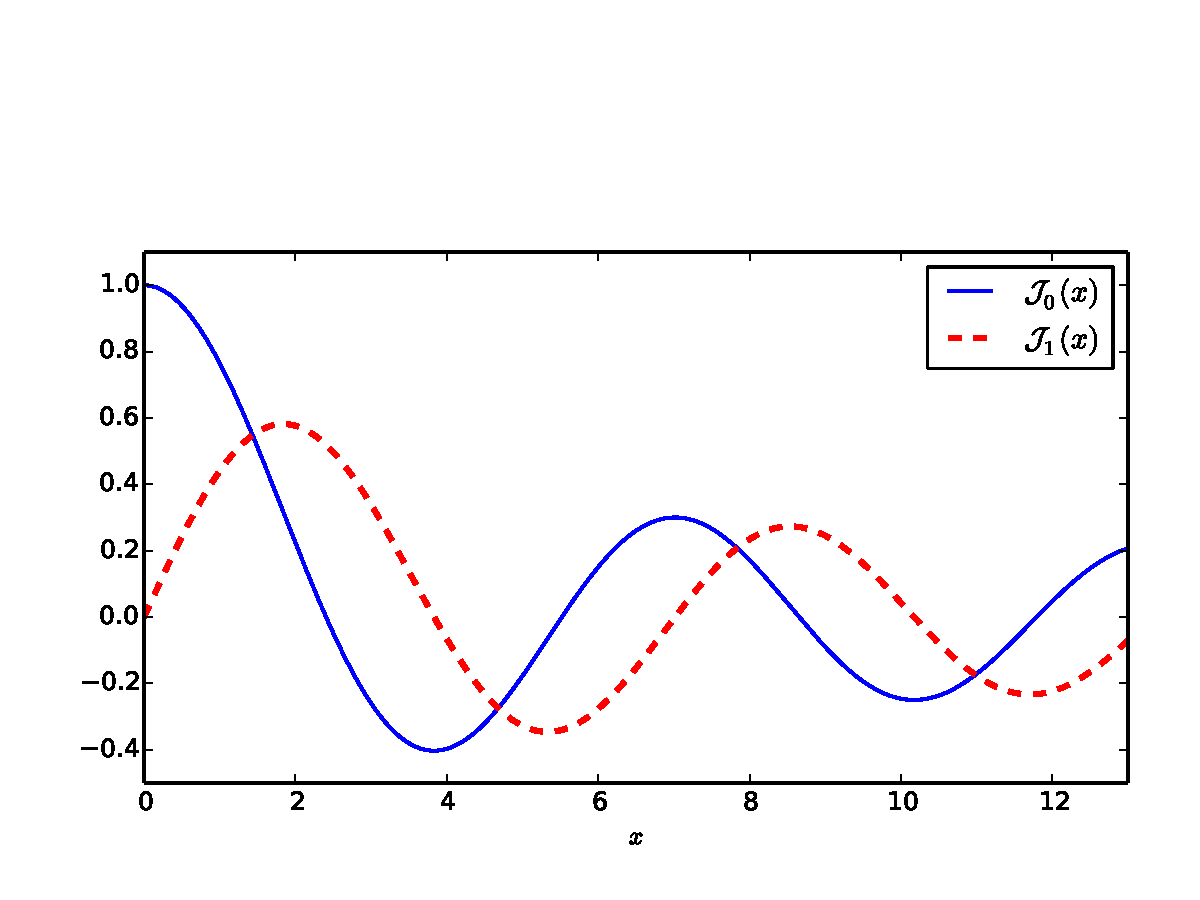
\includegraphics[scale=0.5]{FuncoesdeBesselPrimeiraEspecie.pdf}
\caption{Fun��es de Bessel primeira especie $J_0 $ e $ J_1$.}
\label{f3.1}
\end{figure} 
 
%=====================================================================================================
\subsection{Solu��o Geral para Valores N�o-Inteiros de $\nu$. Solu��o $J_{- \nu}$}
%=====================================================================================================

Dada uma equa��o de Bessel, para termos uma solu��o geral, al�m de $ J_{\nu} $, precisamos tamb�m de uma segunda solu��o linearmente independente de $ J_{\nu} $ (pois a equa��o de Bessel � uma EDO de segunda ordem). % Devemos ter cuidado ao escrever a solu��o geral para a equa��o de Bessel. 
De modo que, se $ s = - \nu $, a segunda solu��o linearmente independente da EDO de Bessel depende de:

$$ s_1 - s_2 = \left\{ \begin{array}{c}
2 \nu \in \mathbb{N} \\
2 \nu \not \in \mathbb{N}\\
\end{array}
\right.$$


%=====================================================================================================
\subsubsection*{Primeiro Caso}
%=====================================================================================================

Se $ 2 \nu \not \in \mathbb{N}  $, ent�o para $ - \nu $, basta substituirmos $ \nu $ por $ - \nu $ em (\ref{Jnu}), ou seja, $ s_2 = - \nu $. Neste caso iremos obter a chamada \textbf{fun��o de Bessel de primeira esp�cie} de ordem $ - \nu $:
\begin{eqnarray}
J_{- \nu} (x) = \sum_{k=0}^{\infty} \frac{(- 1)^k}{ k! \Gamma (1 - \nu + k)} \left( \frac{x}{2} \right)^{2 k - \nu}.
\label{2Jn}
\end{eqnarray}
Dependendo do valor de $ \nu $, a fun��o (\ref{2Jn}) pode conter pot�ncias negativas de $ x $ e ent�o converge em $ \left( 0, \infty \right)  $, deste modo, se trocarmos $ x $ por $  |x| $, as s�ries dadas em (\ref{Jnu}) e (\ref{2Jn}) convergem em $ 0 < |x| < \infty $.


Neste caso, as fun��es $J_{\nu}(x) $ e $J_{- \nu}(x) $ s�o solu��es linearmente independentes em $\left( 0, \infty \right)  $ e a solu��o geral para (\ref{Bessel}) � da forma:
\begin{eqnarray*}
y(x) = c_1 J_{ \nu} (x) + c_2 J_{- \nu} (x); \ \ \ \ \ \ \ \ 0 < |x| < \infty.
\end{eqnarray*}

%\begin{itemize}
%\item Se $ \nu = 0 $, as equa��es (\ref{Jn}) e (\ref{2Jn}) s�o iguais;
%\item Se $ \nu > 0 $ e $s_1 - s_2 = \nu -(- \nu) = 2 \nu $ n�o � um inteiro, ent�o o caso 1 da se��o (\ref{Frobenius}), as fun��es $J_{\nu}(x) $ e $J_{- \nu}(x) $ s�o solu��es linearmente independentes de pel(\ref{bessel}) em $\left( 0, \infty \right)  $, sua solu��o geral neste intervalo � dada por $ y = c_1 J_{ \nu}(x) + c_2 J_{- \nu}(x)  $;
%\item Se $s_1 - s_2 = 2 \nu $ � um inteiro, ent�o poderemos ter uma segunda solu��o em s�rie para (\ref{Bessel}), distinguindo duas possibilidades:

%a) Quando $ \nu = m = inteiro positivo $, a fun��o $J_{- m}(x) $ definida por (\ref{2Jn}) e $J_{ m}(x) $ n�o s�o solu��es linearmente independentes. Podemos mostrar que neste caso $J_{- m}(x) $ � um m�ltiplo de $J_{ m}(x) $.

%b) Quando $ \nu = m = 2 \nu $ pode ser um inteiro quando $ \nu $ for metade de um inteiro �mpar, a fun��o $J_{- m}(x) $ definida por (\ref{2Jn}) e $J_{ m}(x) $ s�o solu��es linearmente independentes, isto �, a solu��o geral para (\ref{Bessel}) em $\left( 0, \infty \right)  $ � dada por $ y = c_1 J_{ \nu}(x) + c_2 J_{- \nu}(x)  $, $ \nu \neq inteiro $. 
%\end{itemize}
\begin{teo.}
%\textbf{Solu��o Geral da Equa��o de Bessel}
Se $ \nu $ n�o for n�mero inteiro, uma solu��o geral da equa��o de Bessel para todo $ x \neq 0 $ �
\begin{eqnarray}
y = c_1 J_{ \nu}(x) + c_2 J_{- \nu}(x).
\label{lll}
\end{eqnarray}
\end{teo.}
\begin{obs.}
Se $ \nu $ for inteiro, ent�o teremos que (\ref{lll}) n�o � uma solu��o geral devido � depend�ncia linear.
\end{obs.}

%=====================================================================================================
\subsubsection*{Segundo Caso}
%=====================================================================================================

Se $ 2 \nu \in \mathbb{N}  $, ent�o poderemos ter uma segunda solu��o na forma,
\begin{eqnarray*}
y_2(x) = c J_{ \nu} (x) ln (x) + \sum_{m=0}^{\infty} b_m x^{m - \nu}; \ \ \ \ (b_m \neq 0),
\end{eqnarray*}
em que $ c $ � uma constante que pode ser zero, isto �, para $ 2 \nu \in \mathbb{N}  $ podemos distinguir duas possibilidade:
\begin{enumerate}
\item  Quando $ \nu = n $, $ n \in \mathbb{Z}  $ pode ser um inteiro quando $ \nu $ for metade de um inteiro �mpar, as fun��es $J_{- n}(x) $ e $J_{ n}(x) $ s�o solu��es linearmente independentes, isto �, a solu��o geral para (\ref{Bessel}) em $\left( 0, \infty \right)  $ � dada por $ y = c_1 J_{ \nu}(x) + c_2 J_{- \nu}(x)  $, $ \nu \neq inteiro $. 
\item  Quando $ \nu = n =$ inteiro positivo, as fun��es $J_{- \nu}(x) $ e $J_{ \nu}(x) $ n�o s�o solu��es linearmente independentes. Pode-se mostrar que neste caso $J_{- n}(x) $ � um m�ltiplo de $J_{ n}(x) $, veja o seguinte teorema: 
\begin{teo.}{(\textbf{Depend�ncia Linear das Fun��es de Bessel $ J_{ \nu}(x)$ e $ J_{- \nu}(x)  $ }) }
Para n�meros inteiros $ \nu = n $, as fun��es de Bessel $ J_{ \nu}(x)$ e $ J_{- \nu}(x)  $ s�o linearmente dependentes, porque
\begin{eqnarray*}
J_{ - n}(x) = (- 1)^{n} J_{n}(x) \ \ \ \ \ \ \ (n \geq 1).
\end{eqnarray*} 
\end{teo.}
\end{enumerate}
\begin{exe.}
A solu��o Geral para a equa��o
\begin{eqnarray*}
x^2 y'' + x y' + \left( x^2 - \frac{1}{4} \right) y = 0,
\end{eqnarray*}
em  $\left( 0, \infty \right)  $ � $ y = c_1 J_{ \frac{1}{2}}(x) + c_2 J_{ - \frac{1}{2}}(x)  $. De fato, pois $
v^2 = \frac{1}{4} \Rightarrow v = \pm \frac{1}{2}.$
\end{exe.}

%=====================================================================================================
\subsection{Fun��o de Bessel de Segunda Esp�cie $ Y_{\nu}(x)$}
%=====================================================================================================

Da �ltima subse��o, vimos que $ J_{\nu}(x)$ e $ J_{ - \nu}(x)$ formam uma base de solu��es da equa��o de Bessel, desde que $ v $ n�o seja um n�mero inteiro. Por�m, quando $ \nu $ � inteiro, essas duas solu��es s�o linearmente dependentes num intervalo qualquer, veja o teorema anterior. Logo, para que tenhamos uma solu��o geral tamb�m nos casos em que $ \nu = n $ � um inteiro, precisamos de uma segunda solu��o linearmente independente, al�m de $ J_{ \nu}(x)$. Essa solu��o � chamada de \textbf{fun��o de Bessel de segunda esp�cie}, vamos denotar por $ Y_{n} $. Obteremos agora uma solu��o dessa fun��o, come�ando com o caso $ n = 0 $.

%=====================================================================================================
\subsection{Fun��o de Bessel de Segunda Esp�cie $ Y_{0}(x)$}
\label{besselss}
%=====================================================================================================

Quando $ \nu = 0 $, podemos escrever a equa��o de Bessel como
\begin{eqnarray}
x y'' + y' + x y = 0.
\label{y0}
\end{eqnarray}
Note que este � o Caso 3 da Se��o (\ref{Frobenius}), onde a equa��o indicial possui uma dupla raiz $ s = 0 $. Desse modo, pelo m�todo de Frobenius, teremos sempre uma solu��o, $ J_{0}(x)$, a segunda solu��o que desejamos deve ter a forma
\begin{eqnarray}
y_2 (x) = J_{0}(x) ln x + \sum_{m=1}^{\infty} b_m x^{m }; \ \ \ \ (b_m \neq 0).
\label{2y2}
\end{eqnarray}
De fato, substituindo ent�o $ y_2 $ e suas derivadas: 
\begin{eqnarray*}
y_2 ' = J_{0} ' ln x + \frac{J_0}{x} + \sum_{n=1}^{\infty} n b_n x^{n - 1 }
\end{eqnarray*}
e
\begin{eqnarray*}
y_2 '' = J_{0} '' ln x + \frac{2 J_0 '}{x} - \frac{J_0}{x^2} + \sum_{n=1}^{\infty} n(n - 1)b_n x^{n - 2 },
\end{eqnarray*}
em (\ref{y0}), obtemos:
\begin{center}
$x \left(  J_{0} '' ln x + \frac{2 J_0'}{x} - \frac{J_0}{x^2} + \sum_{n=1}^{\infty} n(n - 1)b_n x^{n - 2 } \right) + J_{0} ' ln x + \frac{J_0}{x} + \sum_{n=1}^{\infty} n b_n x^{n - 1 } + x  \left( J_{0} ln x + \sum_{n=1}^{\infty} b_n x^{n } \right) = 0$.
\end{center}

\begin{center}
$ \Rightarrow x  J_{0} '' ln x + 2 J_0' - \frac{J_0}{x} + \sum_{n=1}^{\infty} n(n - 1)b_n x^{n - 1 } + J_{0} ' ln x + \frac{J_0}{x} + \sum_{n=1}^{\infty} n b_n x^{n - 1 } + x J_{0} ln x + \sum_{n=1}^{\infty} b_n x^{n + 1 } = 0$. 
\end{center}
Note que os termos $ \frac{J_0}{x} $ e $ - \frac{J_0}{x} $, se cancelam. Da�

\begin{center}
$  l n x \left[ x  J_{0} ''  + J_{0} ' + x J_{0} \right] + 2 J_0' + \sum_{n=1}^{\infty} n(n - 1)b_n x^{n - 1 }  + \sum_{n=1}^{\infty} n b_n x^{n - 1 }  + \sum_{n=1}^{\infty} b_n x^{n + 1 } = 0$. 
\end{center}
Note que, a soma dos termos entre corchetes � zero. De fato, pois $ J_0 $ � uma solu��o de (\ref{y0}). Deste modo ficamos agora com 

\begin{center}
$  2 J_0' + \sum_{n=1}^{\infty} n(n - 1)b_n x^{n - 1 }  + \sum_{n=1}^{\infty} n b_n x^{n - 1 }  + \sum_{n=1}^{\infty} b_n x^{n + 1 } = 0$. 
\end{center}
somando a primeira e a segunda s�rie, obtemos:
\begin{eqnarray}
 2 J_0' + \sum_{n=1}^{\infty} n^2 b_n x^{n - 1 }  + \sum_{n=1}^{\infty} b_n x^{n + 1 } = 0.
\label{bbb}   
\end{eqnarray} 
Lembrando que

\begin{center}
$  J_{0} (x) = \sum_{n=0}^{\infty} \frac{(- 1)^n x^{2 n}}{2^{2 n}( n!)^2} = 1 - \frac{x^2}{2^2 (1!)^2} + \frac{x^4}{2^4 (2!)^2} - \frac{x^6}{2^6 (3!)^2} +- \ldots $.
\end{center}
Segue-se que
\begin{eqnarray*} 
 J_{0}' (x) & = & - \frac{2x}{2^2 (1!)^2} + \frac{4x^3}{2^4 (2!)^2} - \frac{6x^5}{2^6 (3!)^2} +- \ldots \\ \\ & = & - \frac{2x}{2^{2} (1!)^2} + \frac{2. 2x^3}{2^{2.2} (2!)^2} - \frac{2 . 3 x^5}{2^{2.3} (3!)^2} +- \ldots \\ \\& = & \sum_{n=1}^{\infty} \frac{(- 1)^n 2n x^{2 n - 1}}{2^{2 n}( n!)^2} =  \sum_{n=1}^{\infty} \frac{(- 1)^n x^{2 n - 1}}{n!} \frac{2}{2^{2n}} \frac{n}{n!}.
\end{eqnarray*}
Usando $ \frac{n!}{n} = (n - 1)! $ ficamos com 
\begin{eqnarray}
J_{0}' (x) =\sum_{n=1}^{\infty} \frac{(- 1)^n x^{2 n - 1}}{2^{2 n - 1} n! (n - 1)!}
\label{hh} 
\end{eqnarray}
Substituindo (\ref{hh}) na equa��o (\ref{bbb}), obtemos
\begin{eqnarray}
 2 \sum_{n=1}^{\infty} \frac{(- 1)^n x^{2 n - 1}}{2^{2 n - 1} n! (n - 1)!} + \sum_{n=1}^{\infty} n^2 b_n x^{n - 1 }  + \sum_{n=1}^{\infty} b_n x^{n + 1 } = 0. 
\label{zzzz}  
\end{eqnarray}
Vamos abrir as s�ries:

\begin{eqnarray*}
& 2 & \left( - \frac{2x}{2^{2.1} (1!)^2} + \frac{2. 2x^3}{2^{2.2} (2!)^2} - \frac{2 . 3 x^5}{2^{2.3} (3!)^2} +- \ldots \right) \\ \\
& + & \left( b_1 x^0 + 4 b_2 x + 9 b_3 x^2 + 16 b_4 x^3 + 25 b_5 x^4 + 36 b_6 x^5 + \ldots \right) \\ \\
& + & \left( b_1 x^2 + b_2 x^3 + b_3 x^4 + b_4 x^5 + b_5 x^6 + b_6 x^7 + \ldots \right) = 0
\end{eqnarray*} 
 
Note que: $ b_1 = 0 $.
Segue-se:
\begin{eqnarray*}
9 b_3 + b_1 = 0 \Rightarrow 9 b_3 = 0 \Rightarrow b_3 = 0;
\end{eqnarray*}
\begin{eqnarray*}
25 b_5 + b_3 = 0 \Rightarrow 25 b_5 = 0 \Rightarrow b_5 = 0.
\end{eqnarray*}
E assim por diante, temos que a soma dos termos $ b_m $, com subscrito �mpares s�o nulos. 

Vamos agora trabalhar com as pot�ncias de $ x $ �mpares. Igualando a soma dos coeficientes de $ x $ a zero, isso nos dar
\begin{center}
$ 2 \left( - \frac{2}{2^{2.1} (1!)^2} \right) + 4 b_2 = 0 \Rightarrow  b_2 = \frac{1}{4} $.
\end{center}
Para outros valores dos $ b_n $, com subscrito pares, vamos tirar uma rela��o de recorr�ncia entre coeficientes par de $ x $ em (\ref{zzzz}). Fazendo na primeira s�rie $ 2m - 1 = 2k + 1 $, temos $ m = k + 1 $, na segunda s�rie $ m - 1 = 2k + 1 $ e na terceira, $ m + 1 = 2k + 1 $. Portanto, obtemos 
\begin{eqnarray}
\frac{(- 1)^{k + 1}}{2^{2k} (k + 1)! k!} + (2k + 2)^2 b_{2k + 2} + b_{2k} = 0.
\label{relpar}
\end{eqnarray}
Para $ k = 1 $, (\ref{relpar}) fornece
\begin{center}
$ \frac{1}{8} + 16 b_4 + b_2 = 0 \Rightarrow b_4 = - \frac{3}{128}$;
\end{center}
\begin{center}
$\vdots$
\end{center}
\begin{center}
$  b_{2m} = \frac{(- 1)^{m - 1}}{2^{2m} (m!)^2} \left( 1 + \frac{1}{2} + \frac{1}{3} + \ldots + \frac{1}{m} \right) $.
\end{center}
Mostraremos a rela��o acima por indu��o finita. De fato, se $ m = 1 $, j� mostramos que vale. Agora, suponha que � verdade para $ m = k$, isto � 
\begin{center}
$  b_{2k} = \frac{(- 1)^{k - 1}}{2^{2k} (k!)^2} \left( 1 + \frac{1}{2} + \frac{1}{3} + \ldots + \frac{1}{k} \right) $.
\end{center}
Vamos ent�o, provar que � verdade tamb�m para $ m = k + 1 $. De fato, pois de (\ref{relpar}), obtemos:
\begin{eqnarray*}
b_{2k + 2} = \left[  - \frac{(- 1)^{k + 1}}{2^{2k} (k + 1)! k!} - b_{2k} \right] \frac{1}{(2k + 2)^2} = 0.
\end{eqnarray*}
Por hip�tese $ m = k $, vale, segue-se 
\begin{eqnarray*}
b_{2k + 2} = \left[  - \frac{(- 1)^{k + 1}}{2^{2k} (k + 1)! k!} - \frac{(- 1)^{k - 1}}{2^{2k} (k!)^2} \left( 1 + \frac{1}{2} + \frac{1}{3} + \ldots + \frac{1}{k} \right) \right] \frac{1}{(2k + 2)^2} = 0.
\end{eqnarray*} 
Usando o fato que $ (k + 1)! k! = (k + 1)(k!)^2 $. Obtemos:
\begin{eqnarray*}
b_{2k + 2} & = & \left[ \frac{ - (- 1)^{k} (- 1)}{2^{2k} (k + 1)(k!)^2} - \frac{(- 1)^{k} (- 1)^{- 1}}{2^{2k} (k!)^2} \left( 1 + \frac{1}{2} + \frac{1}{3} + \ldots + \frac{1}{k} \right) \right] \frac{1}{(2k + 2)^2} \\ & = & \frac{ (- 1)^{k}}{ (2k + 2)^2 2^{2k} (k + 1)(k!)^2} + \frac{(- 1)^{k}}{ (2k + 2)^2 2^{2k} (k!)^2} \left( 1 + \frac{1}{2} + \frac{1}{3} + \ldots + \frac{1}{k} \right)\\  & = & \frac{(- 1)^{k}}{ (2k + 2)^2 2^{2k} (k!)^2} \left( 1 + \frac{1}{2} + \frac{1}{3} + \ldots + \frac{1}{k} + \frac{1}{(K + 1)} \right) = 0.
\end{eqnarray*}
Note que 
\begin{eqnarray}
(2k + 2)^2 2^{2k} (k!)^2 & = & (4k^2 + 8k + 4)2^{2k} (k!)^2 \nonumber \\ & = & 2^{2k} 2^2(k^2 + 2k + 1) (k!)^2 \nonumber \\ & = & 2^{2k + 2} \left[  \left(  k + 1 \right) \right]^2.
\end{eqnarray}
Portanto, 
\begin{eqnarray*}
b_{2(k + 1)} = \frac{(- 1)^{k + 1 - 1}}{ 2^{2(k + 1)} \left[  \left(  k + 1 \right) \right]^2} \left( 1 + \frac{1}{2} + \frac{1}{3} + \ldots + \frac{1}{k} + \frac{1}{(k + 1)} \right) \ \ \ \  (k = 1, 2, 3, \ldots)
\end{eqnarray*}
Como quer�amos provar. Usando as nota��es curtas, para simplificar nosso estudo aqui consideremos 
\begin{equation}
h_1 = 1 \ \ \ \ \ \ \ h_m = 1 + \frac{1}{2} + \ldots + \frac{1}{m} \ \ \ \ \ \ (m = 2, 3, \ldots).
\label{h1}
\end{equation}
e inserindo (\ref{h1}) e $ b_1 = b_3 = \ldots = 0 $ em (\ref{2y2}), obtemos o seguinte resultado
\begin{eqnarray*}
y_2 (x) & = & J_{0}(x) ln x + \sum_{m=1}^{\infty} b_m x^{m} \\ & = & J_{0}(x) ln x + \sum_{m=1}^{\infty} \frac{(- 1)^{m - 1} h_m }{2^{2m} (m!)^2} x^{m } x^{2m} \\ & = & J_{0}(x) ln x + \frac{1}{4} x^2 - \frac{3}{128} x^4 +- \ldots .
\end{eqnarray*}

Como $J_{0} $ e $y_{2} $ s�o fun��es linearmente independentes, elas formam uma base de (\ref{y0}) para $ x > 0 $. Naturalmente, obtemos uma outra solu��o base. Se substituirmos $ y_2 $ por uma solu��o particular independente na forma $ a( y_2 + bj_0) $, onde $ a \neq 0 $ e $ b $ s�o constantes, obetemos um elemento linearmente independente com $J_{0} $. � uma pratica escolhermos $ a = 2 / \pi $ e $ b = \gamma - l n 2 $, onde o n�mero $ \gamma = 0,57721566490... $ � a \textbf{chamada constante de Euler}, que se define como o limite de 
\begin{eqnarray*}
1 + \frac{1}{2} + \ldots + \frac{1}{s} - l n s
\end{eqnarray*}  
� medida que $ s $ tende ao infinito. A solu��o particular assim obtida � chamada de \textbf{fun��o de Bessel de segunda esp�cie} \textit{de ordem zero} (veja a figura \ref{f3.2}) ou \textbf{fun��o de Neumann } \textit{de ordem zero}, sendo denotada por $ Y_0(x) $. Segue-se que
\begin{eqnarray}
Y_0(x)  = \frac{2}{\pi} \left[ J_0(x) \left(  l n \frac{x}{2} + \gamma \right)  + \sum_{n=1}^{\infty} \frac{(- 1)^{n - 1} h_n }{2^{2n} (n!)^2} x^{2n} \right] . 
\label{n0} 
\end{eqnarray} 
Para pequenos valores de $ x > 0 $, a fun��o $ Y_0(x) $ tem um comportamento parecido com o de $  l n x $, e $ Y_0(x) \rightarrow - \infty $ � medida que $ x \rightarrow 0 $.

%=====================================================================================================
\subsection{Solu��o Geral da Equa��o de Bessel: Fun��es de Bessel de Segunda Esp�cie $ Y_{n}(x)$}
%=====================================================================================================

Para $  \nu = n = 1, 2, \ldots, $ podemos obter uma segunda solu��o atrav�s de manipula��es semelhantes �s que fizemos para $ n = 0 $. Note que esse �  o Caso 2 da Se��o (\ref{Frobenius}), onde as ra�zes indicias diferem por um inteiro, logo a solu��o tamb�m cont�m um termo logar�tmico.
Note que a situa��o n�o est� ainda completamente satisfat�ria, porque a segunda solu��o � definida diferentemente, dependendo da ordem $ \nu $ ser ou n�o um n�mero inteiro. Para darmos unidade ao formalismo, � desej�vel adotarmos uma segunda solu��o-padr�o $ Y_{\nu}(x) $ para todo $ \nu $, consideremos:
\begin{description}
	\item[(i)] Quando $ \nu $ n�o � um inteiro, defina  
\begin{eqnarray}
 Y_{\nu}(x) = \frac{1}{\sin \nu \pi} \left[  J_{\nu}(x) \cos \nu \pi - J_{ - \nu} (x) \right];
\label{7a} 
\end{eqnarray}
	\item[(ii)] Quando $ \nu $ � um inteiro, defina 
\begin{eqnarray}
 Y_n(x) = \lim_{\nu \to n} Y_{\nu}(x). 
\label{7b}
\end{eqnarray}
\end{description}
Essa fun��o � chamada de \textbf{fun��o de Bessel de segunda esp�cie} de ordem $ \nu $ ou \textbf{fun��o de Nemann} de ordem $ \nu $, em que $ Y_n (x) $ n�o tem limite finito quando $ x \rightarrow 0$. A Figura \ref{f3.2} mostra $ Y_0(x)$ e $ Y_1(x)$.
\begin{figure}[!ht]
\centering
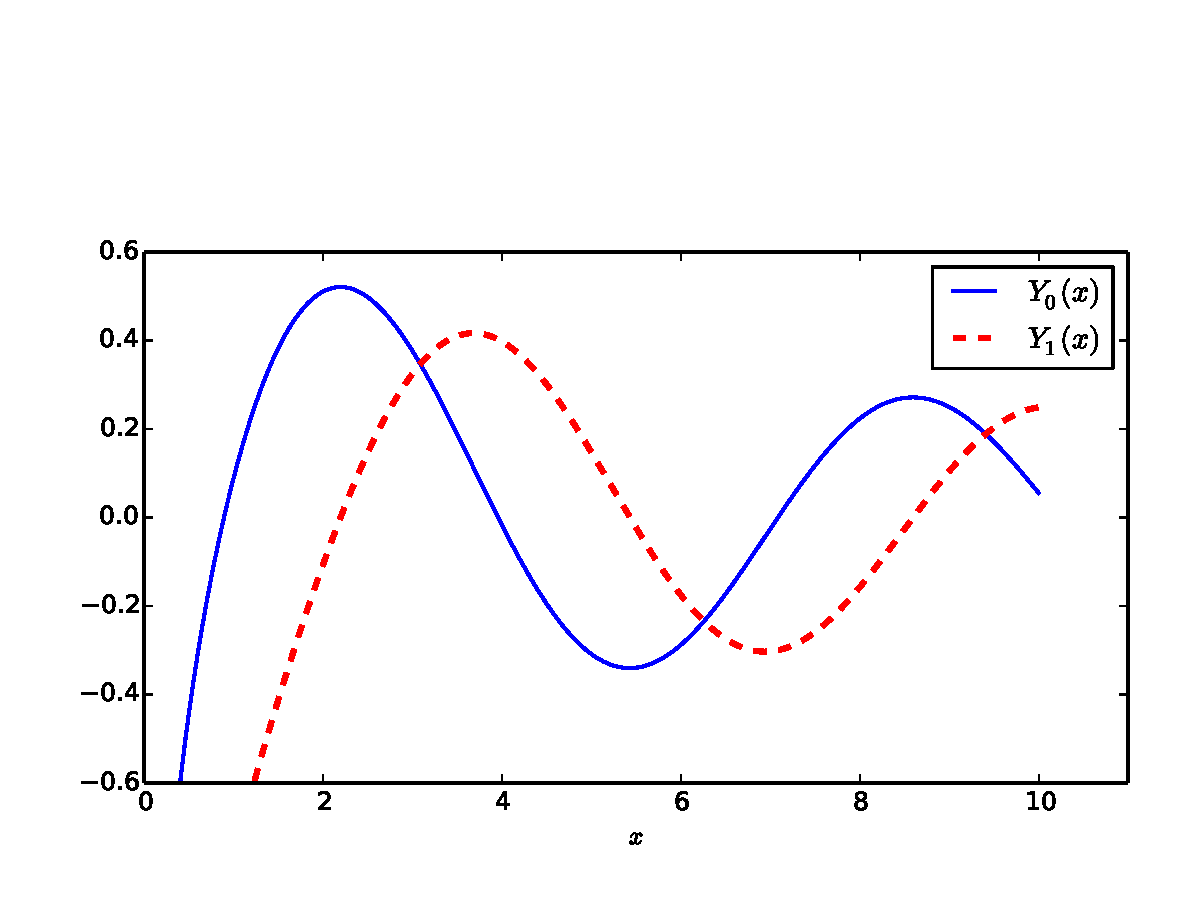
\includegraphics[scale=0.5]{FuncoesdeBesselSegundaEspecie.pdf}
\caption{Fun��es de Bessel segunda especie $Y_0 $ e $ Y_1$.}
\label{f3.2}
\end{figure} 

Donde, $J_{n}(x) $ e $Y_{n}(x) $ s�o solu��es da equa��o de Bessel linearmente independentes. Deste modo, o resultado �: 
\begin{eqnarray}
Y_n(x)  = \frac{2}{\pi} J_n(x) \left(  l n \frac{x}{2} + \gamma \right)  + \frac{x^n}{\pi} \sum_{m=0}^{\infty} \frac{(- 1)^{m - 1} \left( h_m + h_{m + n }\right)}{2^{2m + n} m! ( m + n )! } x^{mn} \nonumber \\ - \frac{x^{- n}}{\pi} \sum_{m=0}^{n - 1} \frac{(n - m - 1)!}{2^{2m - n} m!} x^{2m},
\label{nyn}
\end{eqnarray} 
Onde $ x > 0$, $n = 0, 1, \cdots $ e [como em (\ref{h1})] $h_0 = 0 $, $ h_1 = 1 $,
\begin{eqnarray*}
 h_m = 1 + \frac{1}{2} + \ldots + \frac{1}{m} \ \ \ \ \ \ \ \ \ \ \ \ \ h_{m + n} = 1 + \frac{1}{2} + \ldots + \frac{1}{m + n}. 
\end{eqnarray*}

Consideremos os seguintes resultados:
\begin{description}
	\item[(i)] O limite (\ref{7b}) existe e pode ser mostrado, donde, $Y_{n} $ � uma solu��o da equa��o de Bessel para ordens infinitas,(veja a Ref.\cite{engenharia});
	\item[(ii)] � poss�vel mostrar que as fun��es $J_{n}(x) $ e $Y_{n}(x) $ s�o de fato solu��es da equa��o de Bessel linearmente independentes para todo $ \nu $ e para $ x > 0$;
	\item[(iii)] Dada uma ordem $ \nu $ n�o-inteiro, a fun��o $Y_{\nu}(x) $ � uma solu��o de Bessel. De fato, pois para esses valores de $ \nu $, as solu��es $J_{n}(x)$ e $J_{n}(x)$ s�o solu��es linearmente independentes;  
	\item[(iv)] Observe tamb�m, que em $ n = 0 $, a �ltima soma em (\ref{nyn}) ser� $ 0 $.
Al�m disso, podemos mostrar que 
\begin{eqnarray*}
Y_{- n}(x) = (-1)^n Y_{n}(x).  
\end{eqnarray*}
\end{description}
Agora, podemos considerar como o principal resultado o seguinte Teorema: 

\begin{teo.}{\textbf{Solu��o Geral da Equa��o de Bessel}}

Uma solu��o geral da equa��o de Bessel para todos os valores de $ \nu $ e $ x > 0 $ � 
\begin{equation}
y(x) = c_1 J_{\nu}(x) + c_2 Y_{\nu}(x).
\end{equation}
\end{teo.} 

Consideremos tamb�m, se a vari�vel independente $ x $ em (\ref{bessel}) � substitu�da por $ xk $ ($ k $ constante), a equa��o resultante � (veja a Ref. \cite{calor}):
\begin{eqnarray*}
x_2 y '' + x y '+ ( k^2 x^2 - \nu^2) y = 0,
\end{eqnarray*} 
com solu��o geral 
\begin{eqnarray*}
y(x) = c_1 J_{\nu}(kx) + c_2 Y_{\nu}(kx).
\end{eqnarray*} 
\chapter{Cilindro Infinito}

Se um cilindro de um comprimento l � consideravelmente maior do que o di�metro $ 2R $, ( isto �, $ l / 2 R \gg 1 $ ), ent�o, podemos considera-lo como um cilindro infinito, cujo comprimento � infinitamente maior em compara��o com seu di�metro.

Deste modo, se a transfer�ncia de calor entre a superf�cie do cilindro e o ambiente ocorre uniformemente sobre toda a superf�cie, a sua temperatura vai depender apenas do tempo e do raio (problema sim�trico).

%==================================================================================
\section{Problema Sim�trico}
%==================================================================================

Dado um cilindro infinito consideremos uma distribui��o radial de temperatura prescrita, isto �, na forma da fun��o $ f (r) $, uma fun��o que determina a temperatura inicial de um ponto qualquer no instante inicial $ t = 0 $ dentro do intervalo $ 0 < r < R $.

Observe a seguinte figura:
\begin{figure}[!ht]
\centering
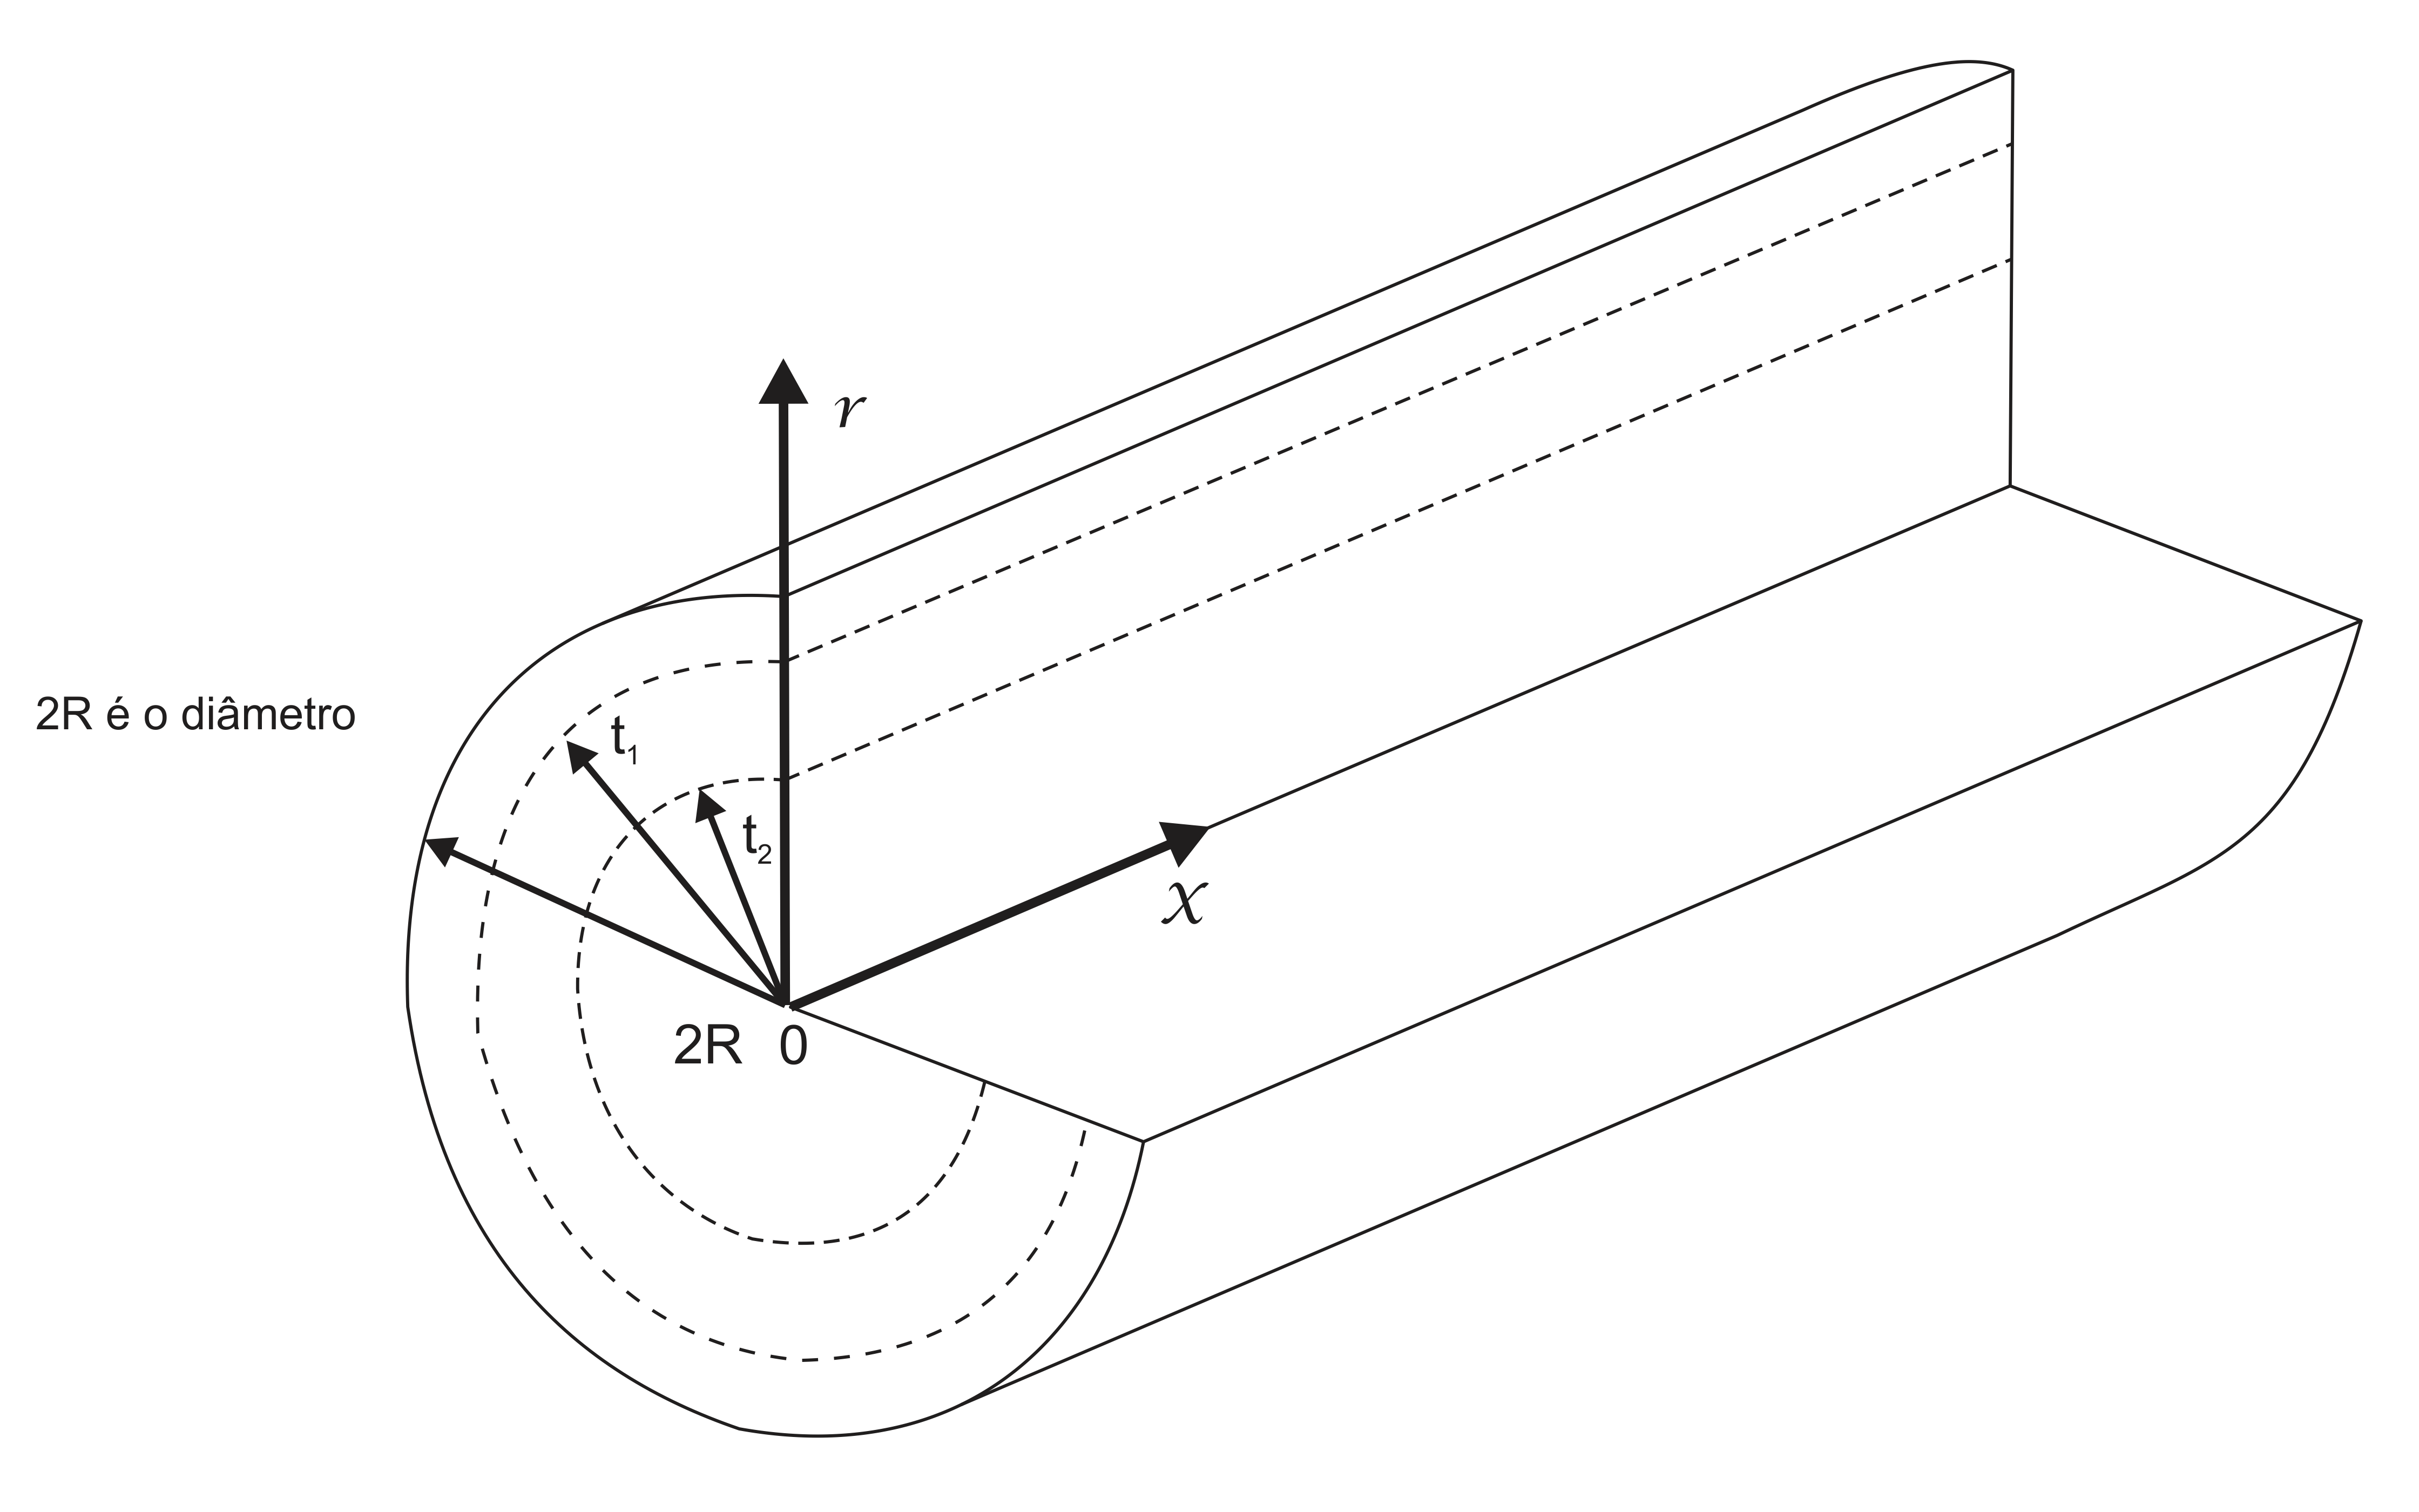
\includegraphics[scale=0.1]{cilindro.png}
\caption{Cilindro infinito com uma distribui��o radial de temperatura prescrita, $ f (r) $, no intervalo $ 0 < r < R $ }
\label{f3.4}
\end{figure}
\newpage
De modo que, no instante de tempo inicial a superf�cie do cilindro � instantaneamente resfriada a alguma temperatura $ t_a $ que � mantida constante durante todo o processo de resfriamento. Logo, a distribui��o de temperatura e a taxa de calor espec�fico s�o descrito como uma fun��o de tempo $t(r, \tau) $. Entretanto, para determinarmos a taxa de calor especifica e a distribui��o de tempo, em um meio � necess�rio resolver a formula��o correta da equa��o de calor.

No nosso caso, ao longo de um cilindro infinito, a equa��o diferencial de condu��o de calor � escrita como: 

\begin{equation}
\frac{\partial t(r, \tau)}{\partial \tau} = a \left( \frac{\partial^2 t(r, \tau)}{\partial \tau^2} + \frac{1}{r} \frac{\partial t(r, \tau)}{\partial \tau} \right), \ \ \ \ \left( \tau > 0; \ \ 0 < r < R \right).
\label{4.1}
\end{equation}
As condi��es de contorno s�o as seguintes (Fig. \ref{f3.3}):
\begin{eqnarray}
t (r, 0) = f(r), \\
\label{4.2}
t (R, \tau) = t_a = constante, \\
\label{4.3}
\frac{\partial t(0, \tau)}{\partial r} = 0, \ \ \ t (0, \tau) \neq \infty.
\label{4.4} 
\end{eqnarray}
 A �ltima condi��o significa que essa temperatura ao longo do eixo do cilindro, durante todo o processo de transfer�ncia de calor, deve ser finito. Veja a Figura \ref{f3.3}.
 
%==================================================================================
\subsection*{Solu��o do Problema por Separa��o de Vari�veis}
%==================================================================================

Na refer�ncia \cite{calor}, mostra-se que a seguinte solu��o particular da equa��o de condu��o de calor atrav�s do m�todo de vari�veis � dada por:
\begin{equation}
t = \vartheta \exp[-a k^2 \tau],
\end{equation}
onde $ \vartheta $ � a solu��o da equa��o diferencial
\begin{eqnarray*}
\nabla^2 \vartheta + k^2 \vartheta = 0.
\end{eqnarray*}
No nosso caso $ \vartheta (x) $ � uma solu��o da \textbf{equa��o de Bessel}
\begin{eqnarray}
\vartheta '' (r) + \left( \frac{1}{r} \right) \vartheta '(r) + k^2 \vartheta (r) = 0,
\label{46}
\end{eqnarray}
a qual podemos, ainda, escreve-l� na forma
\begin{eqnarray}
r \vartheta '' (r) + \vartheta '(r) + k^2 r \vartheta (r) = 0.
\label{47}
\end{eqnarray}
Fazendo $ \vartheta = y(x) $ e substituindo $ k^2 r  $ em (\ref{47}) pela vari�vel independente $ x $. Deste modo, supondo uma solu��o para a equa��o de Bessel:
\begin{eqnarray}
x y '' + y ' + x y = 0,
\label{48}
\end{eqnarray}
na forma de uma s�rie de pot�ncias 
\begin{eqnarray}
y(x) = \sum_{n=0}^{\infty} a_{n} x^{n} = a_{0} + a_{1} x + a_{2} x^{2} + \ldots ; \ \ \ a_n \neq 0. 
\label{49}
\end{eqnarray}
Derivando termo a termo em (\ref{49}), obtemos:
\begin{eqnarray*}
y '(x) & = & \sum_{n=1}^{\infty} n a_{n} x^{n - 1} = a_{1} + 2 a_{2} x + 3 a_{3}^2 x + 4 a_{4} x^{3} + \ldots, \\ y ''(x) & = & \sum_{n=2}^{\infty} n (n - 1) a_{n} x^{n - 2} = 2 a_{2} + 6 a_{3}^2 x + 12 a_{4} x^{2} + \ldots .
\end{eqnarray*}
Substituindo $y (x) $ e suas derivadas $ y '(x) $ e $y ''(x) $ em (\ref{48}). Obtemos:
\begin{eqnarray*}
x \sum_{n=2}^{\infty} n (n - 1) a_{n} x^{n - 2} + \sum_{n=1}^{\infty} n a_{n} x^{n - 1} + x \sum_{n=0}^{\infty} a_{n} x^{n}. 
\end{eqnarray*}
Vamos abrir as s�ries:
\begin{eqnarray*}
\left( 2 a_{2} x + 6 a_{3} x^2 + 12 a_{4} x^{3} + \ldots  \right) + \left( a_{1} + 2 a_{2} x + 3 a_{3} x^2 + 4 a_{4} x^{3} + \ldots \right) \\ + \left( a_{0} x + a_{1} x^2 + a_{2} x^{3} + a_3 x^4 + \ldots \right) = 0.
\end{eqnarray*}
\begin{eqnarray*} 
\Rightarrow a_1 + \left( a_0 + 4 a_{2} \right) x  + \left( a_{1} + 9 a_{3} \right) x^2 + \left( a_2 + 16 a_4 \right) x^3 + \ldots = 0. 
\end{eqnarray*}
\begin{eqnarray}
\Rightarrow a_1 + \left( a_0 + 2^2 a_{2} \right) x + \left( a_{1} + 3^2 a_{3} \right) x^2 + \left( a_2 + 4^2 a_4 \right) x^3 + \ldots = 0.
\label{410}
\end{eqnarray}
Note que $ a_1 = 0 $. Da�
\begin{eqnarray*}
a_1 + 3^2 a_3 = 0 \Rightarrow a_3 = \frac{- a_1}{3^2} = 0.
\end{eqnarray*}
E assim, por diante, temos que a soma dos termos $ a_n $, com subscrito �mpares s�o nulos.  De fato, basta igualarmos a zero a soma de todos coeficientes para cada valor de $ x $, isso nos dar:
\begin{center}
$ a_0 + 2^2 a_2 = 0 \Rightarrow a_2 = - \frac{1}{2^2} a_0$;
\end{center}
\begin{center}
$ a_1 + 3^2 a_3 = 0 \Rightarrow a_3 = \frac{- a_1}{3} = 0$;
\end{center}
\begin{center}
$ a_2 + 4^2 a_4 = 0 \Rightarrow a_4 = - \frac{1}{4^2} a_2 = \frac{1}{2^2 4^2} a_0 $,
\end{center}
e assim por diante. De maneira que: 
\begin{center}
$ a_{n - 2} + n^2 a_n = 0 $.
\end{center}
Substituindo, os valores obtidos para os $ a_n $ em (\ref{49}), teremos: 
\begin{eqnarray}
y(x) = a_{0} \left( 1 - \frac{x^{2}}{2^2} + \frac{x^{4}}{2^2 4^2} - \frac{x^{6}}{2^2 4^2 6^2} + \ldots \right). 
\label{411}
\end{eqnarray}
Segue que, se $ a_0 = 1 $ em (\ref{411}), ent�o, teremos em particular que a equa��o ser� igual a \textbf{fun��es de Bessel primeira esp�cie de ordem $ 0 $}, isto �:
\begin{eqnarray}
J_{0} (x) =  1 - \frac{x^{2}}{2^2} + \frac{x^{4}}{2^2 4^2} - \frac{x^{6}}{2^2 4^2 6^2},
\label{412}
\end{eqnarray}
A segunda solu��o particular da equa��o (\ref{48}) pode ser encontrado usando seguinte f�rmula:
\begin{eqnarray}
y_2(x) = y_1(x) \int \frac{e^{- \int p(x)} dx }{y^{2}_1 (x)} dx,
\end{eqnarray}
onde $ y_1 (x) = J_{0} (x) $ � a primeira solu��o particular de (\ref{48}). Repetindo o mesmo procedimento do Exemplo (\ref{exe36}), obteremos agora:
\begin{eqnarray}
y_2(x) = J_{0} (x) ln x + \frac{ x^2 }{ 2^{2}} - \frac{x^4}{2^2 4^2} \left( 1 + \frac{1}{2} \right) + \frac{x^6}{2^2 4^2 6^2} \left( 1 + \frac{1}{2} \frac{1}{3} \right) - \cdots .
\end{eqnarray}
Normalmente, em vez da fun��o $ y_2(x) $, � utilizado $ Y_0(x) $, chamada \textbf{fun��o de Bessel de segunda esp�cie} de ordem zero (veja a Se��o \ref{besselss}), de modo $ Y_0(x) $ � uma solu��o particular independente de $ y_1(x) $ que esta ligada a $ y_2(x) $ de tal maneira que: 
\begin{eqnarray}
Y_0(x) = \frac{2}{\pi} y_2(x) + \frac{2}{\pi} J_{0} (x) \left(  \gamma - ln 2 \right),
\end{eqnarray} 
onde $ \gamma = 0,5772 $ � a chamada \textbf{constante de Euler}. 

Como as solu��es particulares $ y_1(x) = J_0(x) $ , $ y_2(x) $ ou $ Y_0(x) $ s�o linearmente independente desde que $ Y_0(x)/ J_0(x) \neq const. $, deste modo, a solu��o geral da equa��o Bessel ser�
\begin{equation}
y(x) = c_1  J_0(x) = c_2 Y_0(x),
\end{equation}
onde $c_1 $ e $ c_2$ s�o constantes arbitr�rias.

Consideremos o seguinte resultado, a equa��o (\ref{47}) reduzida a equa��o (\ref{48}) assumindo $ r = x / k $, nos d� a seguinte solu��o para (\ref{47}): 
\begin{equation}
\vartheta (r) = c_1  J_0(kr) + c_2 Y_0(kr),
\end{equation}
uma vez que a temperatura ao logo do eixo do cilindro (r = 0) deve ser finito, a solu��o n�o pode conter a fun��o de Bessel de segunda esp�cie, pois a medida que $ r \rightarrow 0 $, $ Y_0(kr) \rightarrow  - \infty $ (veja a Figura \ref{f3.2}). Assim, a partir das condi��es f�sica do problema, teremos $ c_2 = 0 $.
E a fun��o $ J_0(kr) $ da seguinte forma:  
\begin{eqnarray*}
J_{0} (kr) =  1 - \frac{(kr)^{2}}{2^2} + \frac{(kr)^{4}}{2^2 4^2} - \frac{(kr)^{6}}{2^2 4^2 6^2},
\end{eqnarray*}
a qual satisfaz a condi��o (\ref{4.4}) como
\begin{eqnarray*}
J_{0} ' (kr) & = &  - k \left[ \frac{(kr)}{2} - \frac{(kr)^{3}}{2^2 4} + \frac{(kr)^{5}}{2^2 4^2 6} - \cdots \right] \\ & = & - k j_1 (kr),
\end{eqnarray*} 
visto que, a medida $ r \rightarrow 0$, $ J_{0} ' (kr)$ tamb�m tente a $ 0 $.

N�s iremos encontrar as constantes $k $ e $c_1 $ a partir do limite e condi��es iniciais.

Para simplificar nossos calculo, tomaremos $ t_a = 0$, isto significa, que o ponto de refer�ncia(inicial) da temperatura � $ t_a$. Assim, da condi��o de contorno (\ref{4.3}) em (\ref{st}), obteremos:
\begin{equation*}
t_a = c_1  J_0(kR) \exp[ - a k^2 \tau] = 0.
\end{equation*} 

Conseq�entemente, durante o processo de arrefecimento ($ 0 < \tau < \infty $) devemos considera v�lida a seguinte igualdade
\begin{equation}
J_0 (kR) = 0.
\label{*}
\end{equation}

Esta igualdade � referida como uma fun��o caracter�stica, a partir dela podemos definir os valores $ k_n $.  
 

Esta fun��o $ J_{0} (kR)$ � semelhante a uma fun��o trigonom�trica $  \cos (kR) $ (\ref{f3.1}); temos assim um n�mero infinito de ra�zes $ k_n R = \mu_n $, ou seja, $\mu_1 = 2,4048 $, $\mu_2 = 5,5201  $, $\mu_3 = 8,6537 $ e assim por diante.
Devemos, considerar para grandes valores de $ n $ a diferen�a $ \mu_{n + 1} - \mu_{n} $ est� perto de $ \pi $.

Logo,
\begin{equation}
k_n = \mu_n / R.
\end{equation}
Assim, temos um n�mero infinito de solu��es na forma particular:
\begin{equation}
t = c_1  J_0(k_n r) \exp[ - a k_n^2 \tau].
\label{421}
\end{equation}
Essas solu��es s�o chamadas de fun��es fundamentais. Todos eles v�o ser v�lido n�o s� para a equa��o de difus�o (\ref{4.1}), mas tamb�m para a condi��o contorno (\ref{4.3}).
A solu��o geral ser� uma s�rie na forma:
\begin{equation}
t (r, \tau) = \sum_{n=1}^{\infty} c_n  J_0(k_n r) \exp[ - a k_n^2 \tau].
\label{422}
\end{equation}

Usaremos agora a condi��o inicial (\ref{4.1}) para determinar o valor das constantes $ c_n $, isto �, 
\begin{equation}
t (r, 0) = f(r) = \sum_{n=1}^{\infty} c_n  J_0(k_n r).
\label{423}
\end{equation}
A equa��o (\ref{423}) representa a transforma��o de Fourier-Bessel. Assim, para a determina��o das constantes $ c_n $'s devemos usar o mesmo m�todo como descrito anteriormente, mas, primeiramente devemos provar que o sistema das fun��es $ \sqrt{x} J_0(ax)$,  $ \sqrt{x} J_0(bx)$ � ortogonal.

Apresentaremos as seguintes nota��es:
\begin{equation}
y_1 =  J_0(ax), \ \ \ \ \ \ \ \ y_2 =  J_0(bx)
\label{424}
\end{equation}

As fun��es $J_0(ax) $ e $ J_0(bx)$ satisfazem as equa��es diferenciais apropriados em $ y_1 $. �, portanto, � parte integrante da equa��o
\begin{equation*}
x y'' + y' + a^2 x y = 0, 
\end{equation*}
e $ y_2 $ a parte integrante da seguinte equa��o
\begin{equation*}
x y'' + y' + b^2 x y = 0. 
\end{equation*}
Note que, estas equa��es podem ser escritas como
\begin{equation*}
(x y')' =  - a^2 x y, \ \ \ \ \ \ \ \ (x y')' =  - b^2 x y.
\end{equation*}
Assim, temos
\begin{equation}
(x y_1')' =  - a^2 x y_1,
\label{425} 
\end{equation}
\begin{equation}
(x y_2')' =  - b^2 x y_2.
\label{426}
\end{equation}

Multiplicando, a igualdade (\ref{425}) por $ y_2 $ e a igualdade (\ref{426}) por $ y_1 $. Em seguida, subtraindo-se a segunda a partir da primeira, obtemos (tamb�m respons�vel por igualdade (\ref{424})):
\begin{eqnarray*}
b^2 x y_1 y_2 - a^2 x y_1 y_2 & = & y_2 (x y_1')' - y_1 (x y_2')' \\ & = & y_2 (x y_1'' + x' y_1') - y_1 (x y_2'' + x' y_2') \\ & = &  y_2 (x y_1'') + y_2 (x' y_1') - y_1 (x y_2'') - y_1 (x' y_2') \\ & = & ( y_2 x) y_1'' + (y_2 x') y_1' - (y_1 x) y_2'' - (y_1 x') y_2' \\ & = & ( y_2 x) y_1'' + y_2 y_1' - \left[ (y_1 x) y_2'' + y_1 y_2' \right]   \\ & = & (y_2 x y_1')' - (y_1 x y_2')'  = (y_2 x y_1' - y_1 x y_2')'. 
\end{eqnarray*}
Reescrever essa igualdade, assim, teremos: 
\begin{eqnarray}
(b^2 - a^2) x y_1 y_2 = (y_2 x y_1' - y_1 x y_2')'. 
\label{427}
\end{eqnarray}

Ap�s a integra��o de ambos os lados da igualdade de $ 0 $ a $ x $, temos:
\begin{eqnarray*}
(b^2 - a^2) \int_{0}^{x} x y_1 y_2 = x y_2 y_1' - x y_1 y_2'. 
\end{eqnarray*}
Substituindo as ex-nota��es de (\ref{424}), obtemos:
\begin{eqnarray}
\int_{0}^{x} x J_0(ax)J_0(bx) dx = \frac{bxJ_0(ax)J_1(bx) - axJ_0(bx)J_1(ax)}{b^2 - a^2}, 
\label{428} 
\end{eqnarray}
como
\begin{eqnarray*}
y_1 ' & = & aJ_0' (ax) = - aJ_1 (ax), \\ y_2 ' & = & bJ_0' (bx) = - bJ_1 (bx). 
\end{eqnarray*}


Note que, se $b \rightarrow a  $, o lado direito de (\ref{428}) torna-se uma indefinido do tipo $ 0/0 $. Aplicando a regra L'Hospital, temos:
\begin{eqnarray*}
\int_{0}^{x} x J_0^2(ax) dx & = & \lim_{b \to a} \frac{xJ_0(ax)J_1(bx) + bx^2J_0(ax)J_1'(bx) - ax^2J_0'(bx)J_1(ax)}{2b} 
\\ & = & \frac{1}{2a} \left\lbrace  x J_0(ax) J_1(ax) + a x^2 J_0(ax) \left[  J_0(x) - \frac{J_1(ax)}{ax} \right] + ax^2J_1^2(ax)\right\rbrace ,  
\end{eqnarray*}
desde 
\begin{eqnarray*}
J_0 ' (ax) & = & - J_1 (ax), \\ J_1 ' (ax) & = & J_0 (ax) - (1/ax)J_1(ax). 
\end{eqnarray*}

Consequentemente, finalmente, temos:
\begin{eqnarray}
\int_{0}^{x} x J_0^2(ax) dx = \frac{1}{2} x^2 \left[  J_0^2(ax) + J_1^2(ax) \right].
\label{429} 
\end{eqnarray}

Esta f�rmula � v�lida para todos os valores de $ a $ e $ b $ e vai ser usada mais tarde.

Multiplicando ambos os lados da igualdade (\ref{423}) por $ r J_0 (K_m r) $ onde $ K_m r $ s�o as ra�zes da fun��o $ J_0 (K_m r) $ e integrando nos limites de $  0$ a $ R $:

\begin{eqnarray}
\int_{0}^{R} r f(r) J_0(k_m r) dr & = &  \int_{0}^{R} \sum_{n=1}^{\infty} c_n r J_0(k_n r) J_0(k_m r) dr \nonumber \\ & = & \sum_{n=1}^{\infty} c_n \int_{0}^{R} r J_0(k_n r) J_0(k_m r) dr.
\label{430}
\end{eqnarray}
De acordo com a igualdade (\ref{428}), para $ m \neq n $, temos:
\begin{eqnarray*}
\int_{0}^{R} r J_0(k_n ) r J_0(k_m r) dr  = R \frac{k_m J_o (k_n R) J_1(k_m R) - k_n J_0(k_m R) J_1(k_n R)}{k_m^2 - k_n^2} = 0,
\end{eqnarray*}
pois, $ J_0(k_n R) = J_0(k_m R) = 0 $, (No contorno, veja (\ref{*})). Para $ m = n $, de acordo com a f�rmula (\ref{429}), teremos 
\begin{eqnarray*}
\int_{0}^{R} r J_0^2(k_n r) dr  = \frac{1}{2}R^2 J_1^2(k_n R).
\end{eqnarray*}
Assim, por (\ref{430}), temos
\begin{eqnarray*}
c_n = \frac{(2/R^2)\int_{0}^{R} r f(r) J_0(k_n r) dr }{J_1^2(k_nR)}.
\end{eqnarray*}

Finalmente, a solu��o do nosso problema ser� de forma:
\begin{eqnarray*}
t(r, \tau) = \sum_{n=1}^{\infty} \frac{J_0 (y_n r/R)}{J_1^2(y_n)} \frac{2}{R^2} x \int_{0}^{R} r f(r) J_0(y_n r/R) dr \exp[ - y_n^2{a \tau / R^2}].
\end{eqnarray*}

Apesar do problema solucionado estar aplicado ao resfriamento de um corpo cil�ndrico, este problema pode ser aplicado tamb�m � transfer�ncia de massa. Na figura abaixo, a solu��o encontrada foi utilizada para descrever a perda de �gua de uma banana num processo de desidrata��o osm�tica. 
\begin{figure}[!ht]
\centering
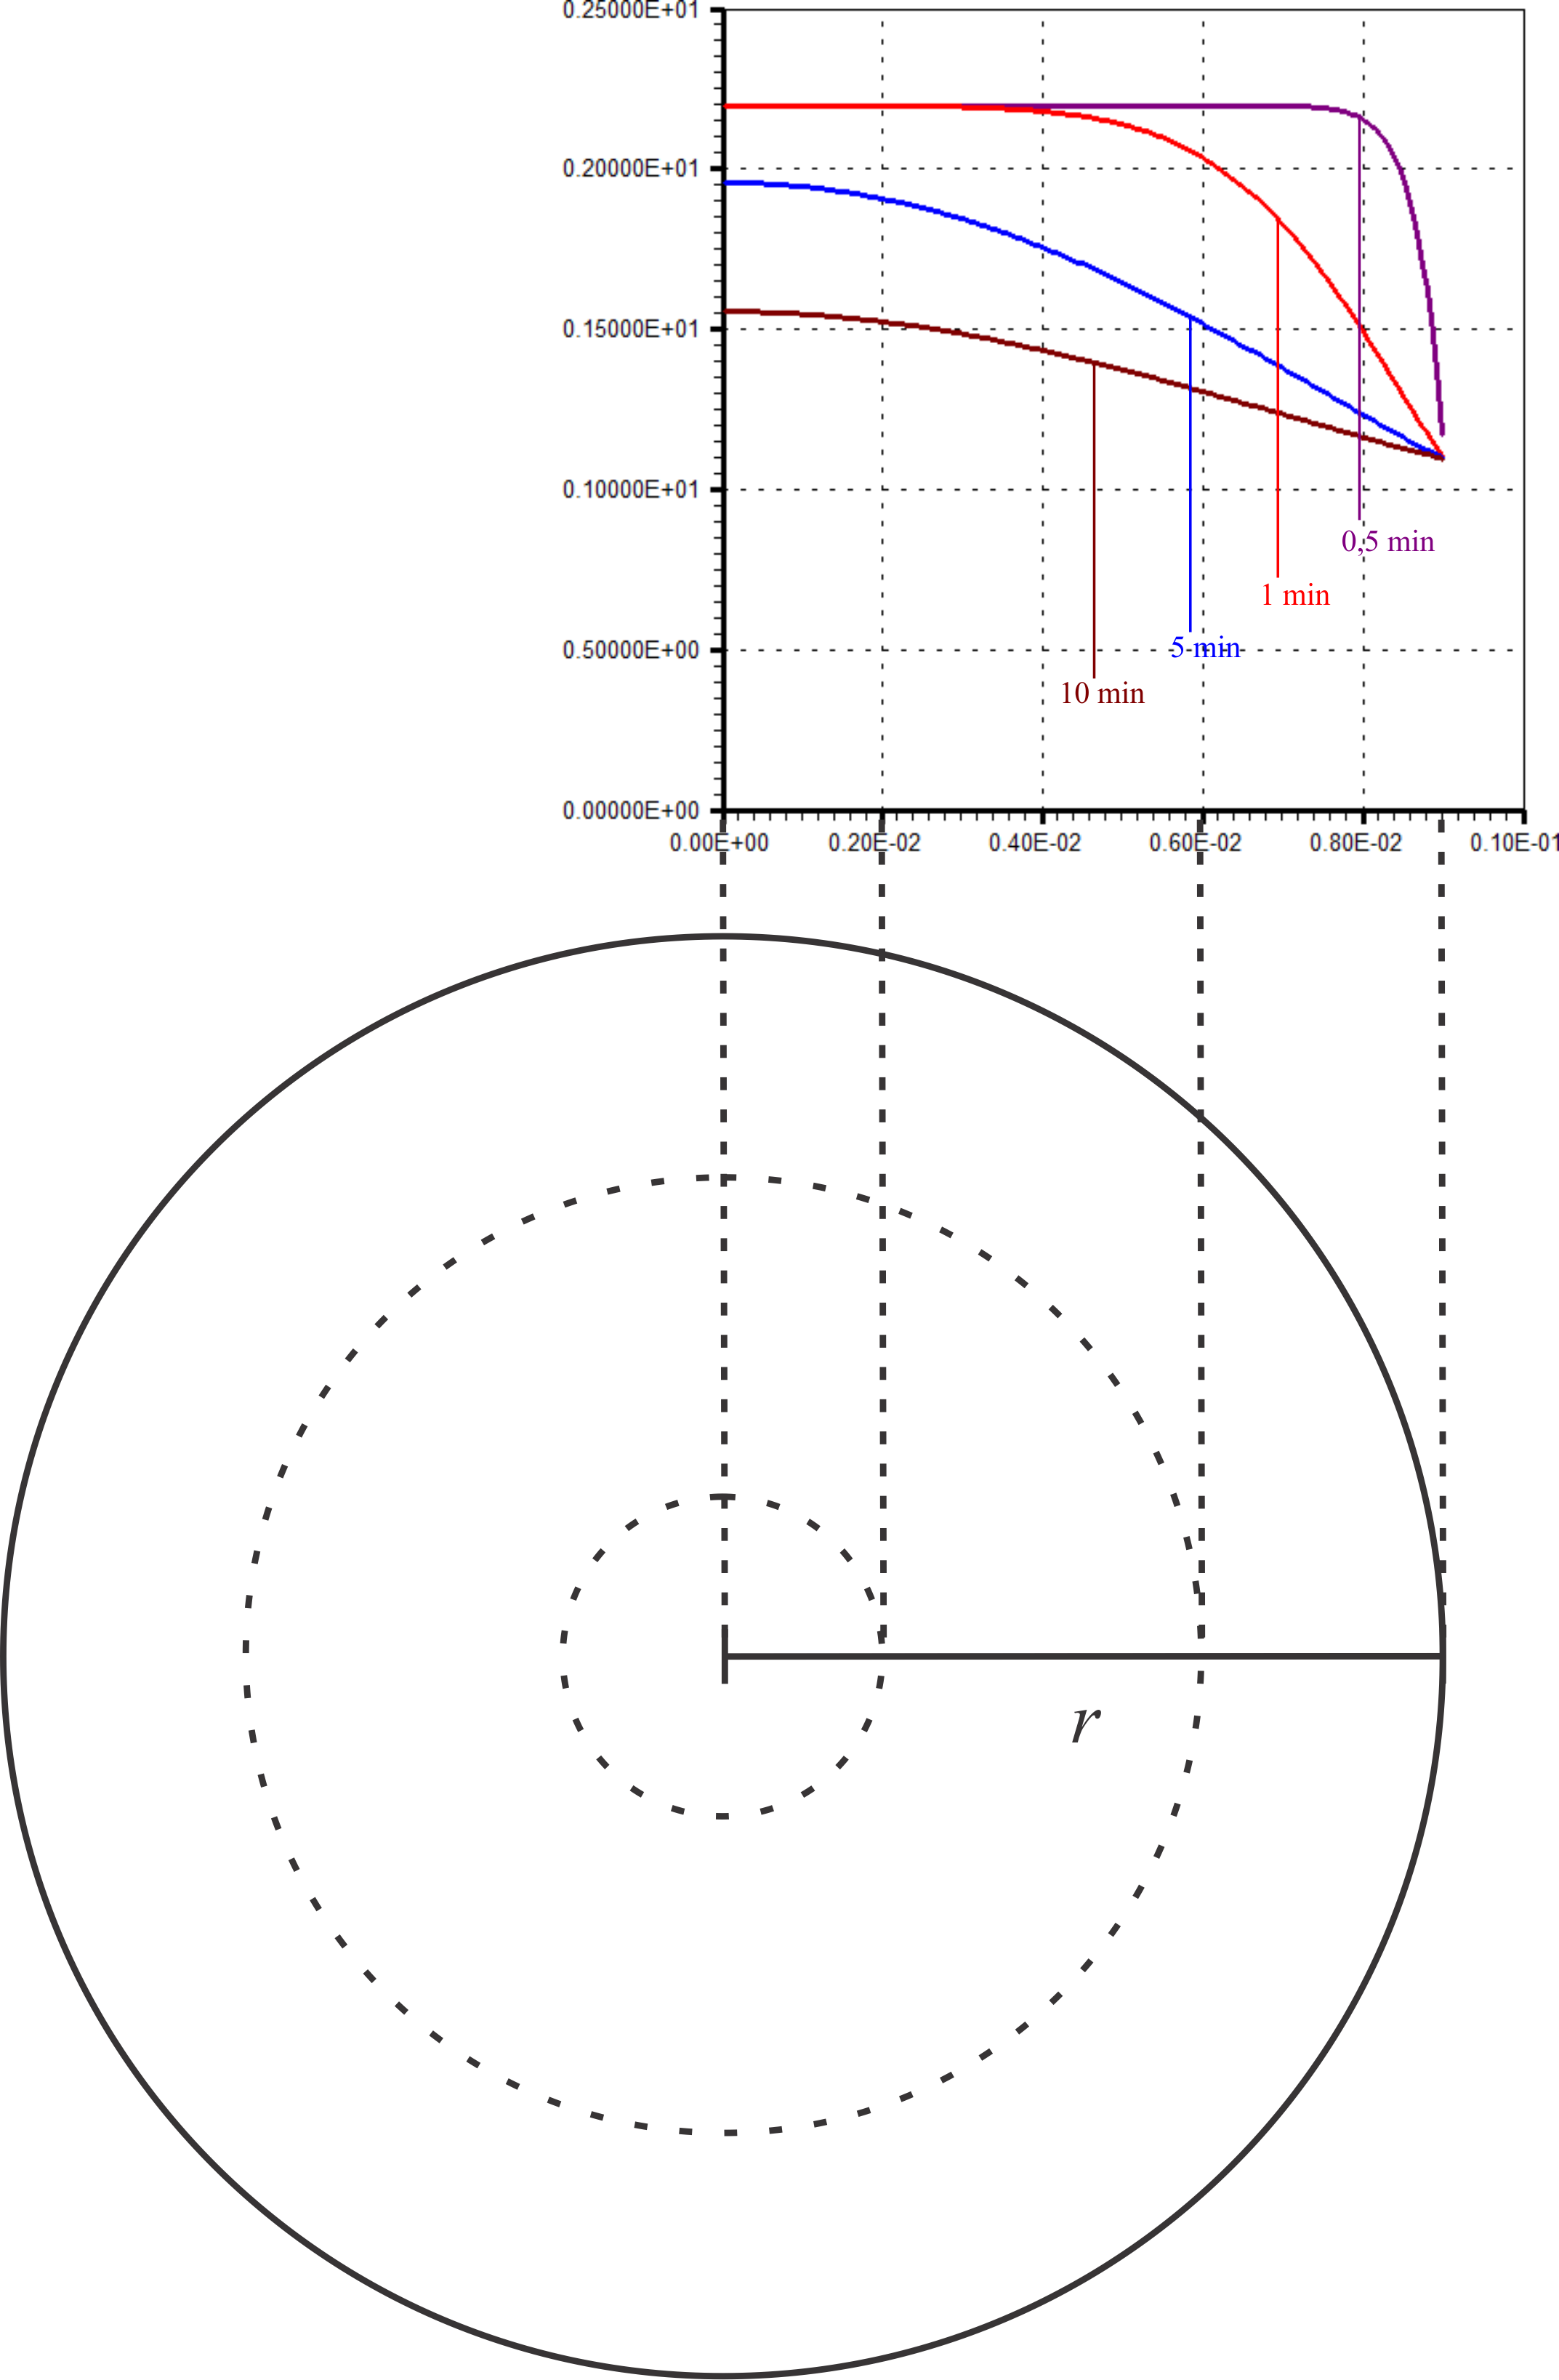
\includegraphics[scale=0.4]{formatado.png}
\caption{Con�trias da perda de �gua de banana num processo de desidrata��o osm�tica}
\label{f3.3}
\end{figure} 
\newpage
\chapter{Conclus�o}

As mais diversas formula��es da equa��o de calor s�o utilizadas para determinar a distribui��o de temperatura em um meio, onde para obtermos a solu��o torna-se necess�rio resolver a formula��o correta. Neste trabalho, apresentamos a formula��o mais geral da equa��o de calor, a equa��o de difus�o. 

A solu��o da equa��o de difus�o para o cilindro infinito tratada em nosso trabalho dependeu das condi��es f�sicas existentes nas fronteiras do meio, isto �, das condi��es de contorno, a qual apresentou um termo que � uma solu��o da equa��o de Bessel.

A equa��o de Bessel surgiu em sua resolu��o particular pelo m�todo da separa��o de vari�veis, donde estabelecemos condi��es para sua solu��o, que embora n�o possuindo coeficientes anal�ticos, foram representadas por meio de uma s�rie de pot�ncias. Analisando uma extens�o do m�todo das s�ries de pot�ncias, aplicando o m�todo de Frobenius, o mesmo nos forneceu a base das solu��es em s�rie, que geralmente trataram-se de EDOs lineares e de segunda ordem, sendo de consider�vel import�ncia pr�tica por tratarmos a equa��o de Bessel em torno de um ponto singular regular.

Apesar do problema aqui estabelecido estar aplicado ao resfriamento de um corpo cil�ndrico, este problema pode ser aplicado tamb�m � transfer�ncia de massa. Dessa maneira, a equa��o de difus�o torna-se uma ferramenta imprescind�vel para a resolu��o de in�meros problemas, sendo poss�vel realizar estudos no que diz respeito � distribui��o da temperatura e o fluxo de calor de um determinado meio.








\addcontentsline{toc}{chapter}{Refer�ncias Bibliogr�ficas}

\begin{thebibliography}{99}

\bibitem{boyce} BOYCE, William E; DIPRIMA, Richard C. \textit{Equa��es Diferenciais Elementares e Problemas de Valores de Contorno}. Tradu��o: Val�ria de Magalh�es I�rio. Rio de Janeiro: LTC, 2006.

\bibitem{engenharia} KREYSZIG, Erwin. \textit{Matem�tica Superior para Engenharia, volume I}. 9 ed. Tradu��o: Lu�s Ant�nio Fajardo Portes; Revis�o T�cnica: Ricardo Nicolau Nassar Koury, Luiz Machado. Rio de Janeiro: LTC, 2013. 

\bibitem{BO} LUIKOV, A. V. \textit{Analytical Heat Diffusion Theory}. Academic Press, Inc. Lid: London, 1968, 685 p. 

%\bibitem{geraldo} �VILA, Geraldo. \textit{An�lise Matem�tica para Licenciatura}. 3 ed. rev. e ampl. S�o Paulo:  BLUCHER, 2006.

\bibitem{SOL} SANTOS, Reginaldo J.. \textit{Exist�ncia de Solu��es de Equa��es Diferenciais em S�rie de Pot�ncias}. Dispon�vel em: \href{https://www.mat.ufmg.br/~regi/eqdif/iedo.pdf}{\texttt{https://www.mat.ufmg.br/~regi/eqdif/iedo.pdf}}. Acesso em: 11 de dezembro de 2014.

\bibitem{eq} COUTO, Roberto Toscano. \textit{Equa��es Diferenciais (GMA00024)}. Dispon�vel em: \href{https://www.professores.uff.br/rtoscano/eqsdif.pdf}{\texttt{https://www.professores.uff.br/rtoscano/eqsdif.pdf}}. Acesso em: 11 de dezembro de 2014.

\bibitem{livronet} ZILL, Dennis G. ; CULLEN, Michael R.  \textit{Matem�tica Avan�ada para Engenharia - Vol I}. 9 ed. S�o Paulo: Bookman, 2009.

\bibitem{elonfino} LIMA, Elon Lages. \textit{An�lise Real vol. 1 - Fun��es de uma Vari�vel Real}. 11 ed. Rio de Janeiro: IMPA -- Cole��o Matem�tica Universit�ria, 2012.

\bibitem{elongrosso} LIMA, Elon Lages. \textit{Curso de An�lise vol. 1}. 13 ed. Rio de Janeiro: IMPA -- Cole��o Projeto Euclides, 2011.

\bibitem{halliday} RESNICK, Robert; HALLIDAY, David; KRANE, Kenneth S. \textit{F�sica 2}. 1 ed. S�o Paulo:  Pioneira Thomson Learning, 2003.

\bibitem{calor} MIRANDA, Felipe Dias de. \textit{Equa��o do Calor}. Dispon�vel em \href{https://metodosmatematicosuff.files.wordpress.com/2011/03/trabalho\\-mc3a9todos.doc}{\texttt{https://metodosmatematicosuff.files.wordpress.com/2011/03/trabalho\\-mc3a9todos.doc}}. Acesso em: 01 de junho de 2015.

%\bibitem{pontosingulares} UFRGS (Instituto de F�sica). \textit{Se��o 27: Pontos Singulares. M�todo de Frobenius
%}. Dispon�vel em: \href{https://www.mat.ufrgs.br/~brietzke/textos/secao27_2011_2.pdf}{\texttt{https://www.mat.ufrgs.br/~brietzke/textos/secao27_2011_2.pdf}}. Acesso em: 09 de outubro de 2015.
\bibitem{resumo} Instituto Tecnol�gico de Aeron�utica - ITA (Departamento de Matem�tica). \textit{RESOLU��O DE EDO'S POR SERIES (RESUMO)}. Dispon�vel em: \href{http://www.mat.ita.br/~botelho/sites/default/files/resumo32wk16.pdf}{\texttt{http://www.mat.ita.br/~botelho/sites/default/files/resumo32wk16.pdf}}. Acesso em: 04 de fevereiro de 2015.

\bibitem{Fespeciais} OLIVEIRA, Edmundo Capelas de. \textit{Fun��es Especiais com Aplica��es}. 1 ed. S�o Paulo: Editora Livraria da Fisica, 2005.

\bibitem{thomas2} WEIR, Maurice D.; HASS, Joel; GIORDANO, Frank R. \textit{C�lculo (George B. Thomas Jr.), volume II}. 11 ed. Tradu��o: Luciana do Amaral Teixeira, Leila Maria Vasconcelos Fiqueiredo; Revis�o T�cnica: Cl�udio Hirofume Asano. S�o Paulo: Pearson, 2009.

\bibitem{condutividadefisicanet} VILCHES, Mauricio A..\textit{EQUA��ES DIFERENCIAIS:
M�TODOS DE S�RIES}. Dispon�vel em: \href{https://aiecp.files.wordpress.com/2012/07/calculo4.pdf}{\texttt{https://aiecp.files.wordpress.com/2012/07/calculo4.pdf}}. Acesso em: 09 de junho de 2015.

\bibitem{FHamonica} FURTADO, Marcelo A..\textit{Notas de EDP2
(vers�o 1.2)}. Dispon�vel em: \href{http://www.mat.unb.br/~furtado/homepage/notas-edp2.pdf}{\texttt{http://www.mat.unb.br/~furtado/homepage/notas-edp2.pdf}}. Acesso em: 13 de novembro de 2015.
\label{refr}

\bibitem{Reais} GALDINO, Andr� Luiz.\textit{Sequ�ncias de N�meros Reais}. Dispon�vel em: \href{https://galdino.catalao.ufg.br/up/635/o/sequencia.pdf}{\texttt{https://galdino.catalao.ufg.br/up/635/o/sequencia.pdf}}. Acesso em: 29 de novembro de 2015.
\label{refr} 

\end{thebibliography} 
\end{document}
